%!TEX root = Manuscript.tex

\chapter{Rough co-registration}
\label{chap:RoughCoReg}
\minitoc

\section{Introduction}
\subsection{Motivation and objective}
The goal of rough co-registration is to perform rough alignment between image pairs, so that they can be later used to guide the precise matching by narrowing down the search space in 2D image geometry. It plays a fundamental role as wrongly aligned results would lead to deviation from the right search space. Therefore robustness is the most critical target in rough co-registration. In the meantime, it doesn't need to be very accurate as the precision would be improved in the precise matching part via searching local neighborhood. Therefore, we can reasonably sacrifice precision when necessary to trade for robustness.\\

The task of rough alignment could be accomplished by matching every possible inter-epoch image pair, followed by a RANSAC routine to recover the best transformation model between each image pair.
%The task of moving multi-epoch to the same frame could be accomplished by building transformation models from one epoch to another. Generally, every inter-epoch image pair would be matched, followed by a RANSAC routine to recover the best transformation model between each image pair.
However, inter-epoch image pairs often demonstrate different appearances due to scene changes and heterogeneous acquisition conditions, which often leads to limited inlier ratio, in other words, failure of the later RANSAC procedure. Therefore, instead of aligning a group of inter-epoch image pairs separately, we come up with an idea to improve robustness by aligning the whole block integrally to build a globally consistent transformation model. Afterwards, we can move different epochs to the same coordinate frame, providing orientations and \ac{DSM}s in the same geographic system for later processing (i.e., precise matching and \ac{BBA}). Besides, we take advantage of 3D geometry which could be easily obtained within each epoch to boost the inter-epoch matching performance.\\
As a consequence, we come up with 2 strategies for multi-epoch rough co-registration: (1) \textit{ImgPairs} (i.e., matching image pairs) and (2) \textit{Ortho} or \textit{DSM} (i.e., matching orthophotos or \ac{DSM}s). \zll{The former strategy comes up first, but its performance is less satisfactory. This motivated us to conceive and explore the latter strategy.} Even though \textit{ImgPairs} is generally outperformed by \textit{Ortho} or \textit{DSM}, it still has its own strengths in certain cases such as viability for terrestrial images.\\
%\begin{enumerate}
%    \item \textit{ImgPairs}: Match every possible combination of inter-epoch image pairs, followed by projecting the matches onto ground and merging them in order to build globally consistent 3D Helmert transformation model in a RANSAC routine.
%    \item \textit{Ortho} or \textit{DSM}: (1) Generate orthophoto or DSM for each epoch; (2) match orthophoto or DSM pairs, followed by RANSAC based on 2D similarity transformation model to remove outliers; (3) project inlier mathces onto ground to build a 3D Helmert transformation model between epochs. 
%\end{enumerate}

\subsection{Contributions}
%\zll{Our main contribution is integrating the following points into establishing a pipeline for rough co-registration between inter-epoch image pairs:\\}
Our main contribution is complete and fully automated pipelines for rough co-registration between inter-epoch image pairs. The pipelines are composed of the following key ingredients:
\begin{enumerate}
	\item improving matching robustness by building globally consistent transformation model;%, which can be achieved by either (1) matching each inter-epoch image pair separately followed by global filtering or (2) integrating images from the same epoch into a single image (\ac{DSM} or orthophoto) before matching;
	\item introducing the idea of matching \ac{DSM}s to obtain robust matches even under drastic scene changes, as the 3D landscape often stays globally stable over time;
	\item introducing RANSAC in 3D for \textit{ImgPairs}: each three matches projected to \ac{DSM} serve to compute a 3D Helmert transformation model between epochs, and most importantly provide a 2D constraint on all image pairs;
	\item introducing \textit{4 rotation hypotheses} to make SuperGlue suitable for matching images with rotation larger than 45$^\circ$;
	\item introducing \textit{one-to-many tiling scheme} to scale-up the deep learning methods for feature matching;
	\item improving the performance of matching inter-epoch images with SIFT by (1) using downsampled images and (2) skipping ratio test.% and FIGNN.
\end{enumerate}


%\subsection{Motivation}
%\subsection{Contribution}

\section{Methodology}
%Our goal is to improve robustness by building globally consistent transformation model over the whole block.
%In order to achieve this goal, we exploded 2 strategies:
%(1) matching each potential image pair followed with global filtering based on 3D RANSAC;\\
%(2) get a global image for each epoch first (DSM or orthophoto), apply matching and 2D RANSAC.\\
%零碎匹配,整体inlier
%整体匹配
To roughly co-register different epochs to the same frame, we propose 2 strategies: \\
\begin{enumerate}
	\item \textit{ImgPairs}: matching each inter-epoch image pairs followed by global filtering over the whole block;
	\item \textit{Ortho} or \textit{DSM}: generating global image for each epoch (i.e., orthophotos or \ac{DSM}s) and performing matching only once. 
\end{enumerate}
%The recovered matches would be used to build a 3D Helmert transformation model between epochs. 
%We aim at roughly co-register different epochs to the same frame. 
%We provide 2 strategies for inter-epoch rough co-registration: matching image pairs (\textit{ImgPairs}) or matching orthophotos/\ac{DSM}s (\textit{Ortho} or \textit{DSM}). 
%The pipelines will be elaborated in the following sections. 
Please notice our pipelines are generic, different feature matching methods can be readily applied. At present we adopt either SIFT or SuperGlue in our pipeline as they are currently the \textit{state-of-the-art}, but they can be replaced when better matching methods arise in the future.\\
%Not only our methods are able to match aerial or satellite images, but also they are able to match mixed images. 
\zll{Our pipelines are able to match both aerial and satellite images.} For aerial images, they are supposed to be accompanied with focal lengths and physical sensor sizes, which are usually available, as mentioned in Section \ref{chap:intro}. 
\par
We adopt the following naming conventions: (1) $I^{e_1}$ and $I^{e_2}$: images acquired in \textit{epoch$_1$} and \textit{epoch$_2$}; (2) $O^{e_1}$ and $O^{e_2}$: orientations of \textit{epoch$_1$} and \textit{epoch$_2$}; (3) $Op^{e_1}$ and $Op^{e_2}$: orthophotos of \textit{epoch$_1$} and \textit{epoch$_2$}; (4) $D^{e_1}$ and $D^{e_2}$: \ac{DSM}s of \textit{epoch$_1$} and \textit{epoch$_2$}.\\
%\begin{enumerate}
%    \item Images acquired in \textit{epoch$_1$} and \textit{epoch$_2$} are denoted as $I^{e_1}$ and $I^{e_2}$;
%    \item Orientations of \textit{epoch$_1$} and \textit{epoch$_2$} are denoted as $O^{e_1}$ and $O^{e_2}$; 
%    %\item Ground extent of \textit{epoch$_1$} and \textit{epoch$_2$} are denoted as $G^{e_1}$ and $G^{e_2}$;
%    \item Orthophotos of \textit{epoch$_1$} and \textit{epoch$_2$} are denoted as $Op^{e_1}$ and $Op^{e_2}$; 
%    \item DSMs of \textit{epoch$_1$} and \textit{epoch$_2$} are denoted as $D^{e_1}$ and $D^{e_2}$.
%\end{enumerate}
Prior to inter-epoch rough co-registration, we process each epoch individually to recover the relative orientations and \ac{DSM} within the same epoch. It is a standard photogrammetry or \ac{SfM} pipeline and can be accomplished with lots of solutions (e.g., MicMac~\cite{deseilligny2011apero}, COLMAP~\cite{schonberger2016structure}, {OpenMVG~\cite{openMVG}, Theia~\cite{theia}, etc.}). The one used in our experiment is MicMac. It is performed within each \textit{epoch$_i$} individually as follows:
\begin{enumerate}
\item Extract intra-epoch matches between images $I^{e_i}$ with SIFT ~\cite{lowe2004distinctive};
\item Based on the sequential \ac{SfM} to compute interior and relative orientations ({$O_{ini}^{e_i}$}) for aerial images, or to refine the \ac{RPC} for satellite images;
\item Based on image orientations $O_{ini}^{e_i}$, perform semi-global dense matching~\cite{mpd:06:sgm} {between images $I^{e_i}$} to get {\ac{DSM} ($D_{ini}^{e_i}$) in their arbitrary coordinate frames.}
\item Orthorectify the images to get orthophotos ($Op_{ini}^{e_i}$) if strategy \textit{Ortho} is applied.
%\item Project the images onto mean elevation plane ($G_{ini}^{e_i}$) get orthophotos ($Op_{ini}^{e_i}$).
\end{enumerate}
%Please notice that the step (1) and (2) would not be necessary if the epoch is satellite, since the orientations would be provided by RPC(Rational Polynomial Coefficient).\\
%Two different strategies are provided to perform the rough co-registration. The pipelines will be elaborated in the following sections. 
\subsection{Strategy 1: Matching image pairs (\textit{ImgPairs})}
%\subsection{Strategy 1: global filtering}
%CoReg-R3D
%This method is for co-registering aerial epochs only. It is not practical for satellite images as they are often with large size and will decrease efficiency remarkably.\\
The strategy \textit{ImgPairs} is the first attempt we made for rough co-registration. %by matching every possible inter-epoch image pairs separately, followed by estimating a globally consistent transformation model between different epochs over the whole block. 
The workflow is displayed in Figure~\ref{WorkflowImgPair}(a). For the sake of simplicity, only 2 epochs are present in our processing flows, however, it can be easily extended to more epochs. The matching procedure (i.e., the magenta rectangle in Figure~\ref{WorkflowImgPair}(a)) with SIFT or SuperGlue is slightly different, so we elaborate both in Figure~\ref{WorkflowImgPair}(b) and (c) individually for better understanding. We introduce \textit{4 rotation hypotheses} when feature matching method that is not invariant to rotations lager than 45$^\circ$ (e.g., SuperGlue) is applied.\\
%The advantage of the strategy \textit{ImgPairs} is that it often gets more numerous matches than the strategy \textit{Ortho} or \textit{DSM}, as they have higher resolution. However, it leads to lower efficiency in the meantime.\\
\paragraph{\textit{Four rotation hypotheses}.} It normalizes rotation to achieve invariance, which is similar to ASIFT \cite{morel2009asift} by exploring the space of possible deformation, but adapted as it only explores 2D rotation.\\
The \textit{4 rotation hypotheses} works as follows (cf. Figure~\ref{WorkflowImgPair}(d)): 
\begin{enumerate}
    \item Rotate the secondary image by 90$^{\circ}$ four times;
    \item Match each rotated image with the master image;
    \item Keep the rotation hypothesis with the largest number of matches.
\end{enumerate}
%The \textit{4 rotation hypotheses} would not be applied when rotation invariant matching method (e.g., SIFT) is adopted.
\par
\paragraph{Workflow of \textit{ImgPairs}.} Assuming the numbers of images in \textit{epoch$_1$} and \textit{epoch$_2$} are P and Q individually, the strategy \textit{ImgPairs} works as follows:\\
\begin{enumerate}
    \item Match P$\times$Q inter-epoch image pairs respectively, giving rise to P$\times$Q sets of matches $M({\mathbf{K}^{e_1},\mathbf{K}^{e_2}})$ ($\mathbf{K}^{e_i}$ represents keypoints in image $I^{e_i}$).
    \item Sample matches $M({\mathbf{K}^{e_1},\mathbf{K}^{e_2}})$ iteratively to compute the 2D similarity transformation RANSAC model:
    \begin{equation}
    \left [ \begin{array}{c}
    {K}_x^{e_2}\\
    {K}_y^{e_2}
    \end{array}
    \right ] =\lambda \cdot { \left[ \begin{array}{cc}
    	cos\theta & sin\theta\\
    	-sin\theta & cos\theta
    	\end{array} 
    	\right ]} \cdot {\left [ \begin{array}{c}
    	{K}_x^{e_1}\\
    	{K}_y^{e_1}
    	\end{array}
    	\right ]} + \left [ \begin{array}{c}
    \Delta_x\\
    \Delta_y
    \end{array}
    \right ]. \label{eq:2DSim}
    \end{equation}
    where $\lambda$ is the scale factor, $\theta$ is the in-plane rotation angle and $\left [ \begin{array}{c}
    \Delta_x, \Delta_y
    \end{array}
    \right ]$ $^{^T}$ is the translation vector.
    Matches within $T_r$ of its predicted position (i.e., $\lvert \mathbf{K}^{e_2} - (\lambda \cdot {\left[ \begin{array}{cc}
    		cos\theta & sin\theta\\
    		-sin\theta & cos\theta
    		\end{array} 
    		\right]} \cdot \mathbf{K}^{e_1} + \Delta) \rvert < T_r$) are considered as inliers. The resulted inliers are referred to as $M({\mathbf{\widetilde{K}}^{e_1},\mathbf{\widetilde{K}}^{e_2}})$ ($\mathbf{\widetilde{K}}^{e_i}$ represents keypoints in image $I^{e_i}$).\\
    %\item For each image pair, run RANSAC based on 2D similarity transformation model, giving rise to P$\times$Q sets of matches $M({\mathbf{\widetilde{K}}^{e_1},\mathbf{\widetilde{K}}^{e_2}})$ ($\mathbf{\widetilde{K}}^{e_i}$ represents keypoints in image $I^{e_i}$).\\
    This step aims to reduce matches into a reasonable number when SIFT is applied, otherwise the subsequent global filtering would become prohibitive. It is not necessary if SuperGlue is applied as it simultaneously performs filtering during the matching procedure. %matching methods that simultaneously performed filtering during the matching procedure (e.g., SuperGlue) are applied in the previous step.)
    \item Project $\mathbf{\widetilde{K}}^{e_i}$ from SIFT or $\mathbf{K}^{e_i}$ from SuperGlue onto \ac{DSM} $D_{ini}^{e_i}$ with the help of orientations $O_{ini}^{e_i}$, resulting in 3D points $\mathbf{KG}^{e_i}$.
    \item Sample matches $M({\mathbf{KG}^{e_1},\mathbf{KG}^{e_2}})$ iteratively to compute the 3D Helmert transformation RANSAC model:
\begin{equation}
\left [ \begin{array}{c}
{KG}_x^{e_2}\\
{KG}_y^{e_2}\\
{KG}_z^{e_2}
\end{array}
\right ] =\lambda \cdot \mathbf{R} \cdot {\left [ \begin{array}{c}
    {KG}_x^{e_1}\\
    {KG}_y^{e_1}\\
    {KG}_z^{e_1}
    \end{array}
    \right ]} + \left [ \begin{array}{c}
\Delta_x\\
\Delta_y\\
\Delta_z
\end{array}
\right ]. \label{eq:3DSim}
\end{equation}
    
%   \begin{equation*}
%       {KG_i^{e_2}} = \lambda \cdot \mathbf{R} \cdot {KG_i^{e_1}} + \mathbf{T} , \quad i \in [1,3] \label{eq:3Dsim}
%   \end{equation*}
where $\lambda$ is the scale factor, $\mathbf{R}$ is the rotation matrix and $\left [ \begin{array}{c}
    \Delta_x, \Delta_y, \Delta_z
\end{array}
\right ]$ $^{^T}$ is the translation vector.
%We set the number of RANSAC iterations to 1000, and consider matches within $T_r$ of its predicted position as inliers. In our experiment, {$T_r$ was set to 50m.}
\zll{Matches within $T_r$ of its predicted position (i.e., $\lvert \mathbf{KG}^{e_2} - (\lambda \cdot \mathbf{R} \cdot \mathbf{KG}^{e_1} + \Delta) \rvert < T_r$) are considered as inliers.}
    % to find the best 3D Helmert transformation model.
\end{enumerate}

\begin{figure*}[htbp]
    \begin{center}
        \subfigure[Workflow of \textit{ImgPairs}]{
    \begin{minipage}[t]{1\linewidth}
        \centering
        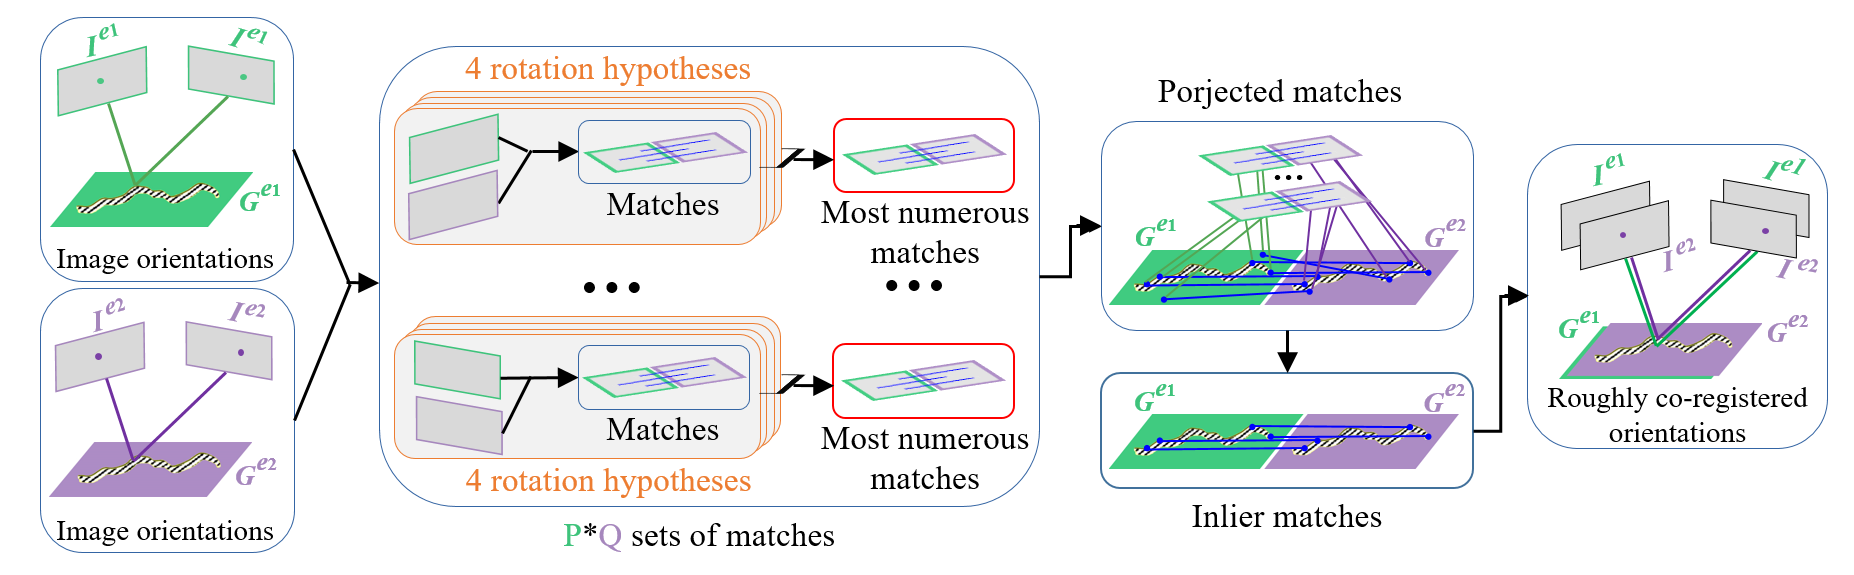
\includegraphics[width=1\columnwidth]{images/Chapitre3/R3D.png}
    \end{minipage}%
}
	\subfigure[Match image pairs with SIFT]{
		\begin{minipage}[t]{0.45\linewidth}
			\centering
			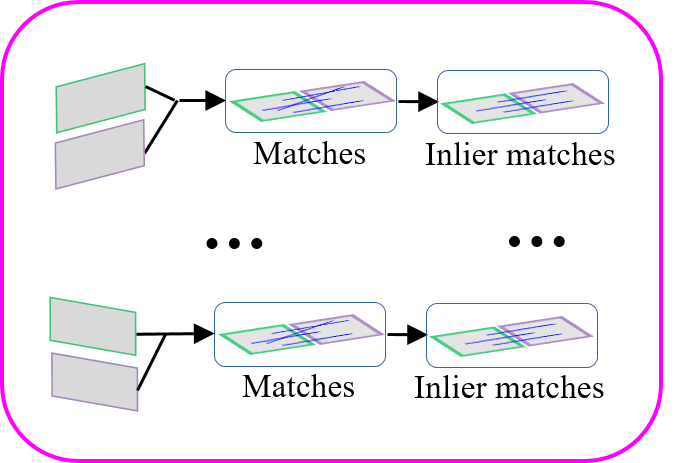
\includegraphics[width=5cm]{images/Chapitre3/R3D-sift.png}
		\end{minipage}%
	}
	\subfigure[Match image pairs with SuperGlue]{
		\begin{minipage}[t]{0.45\linewidth}
			\centering
			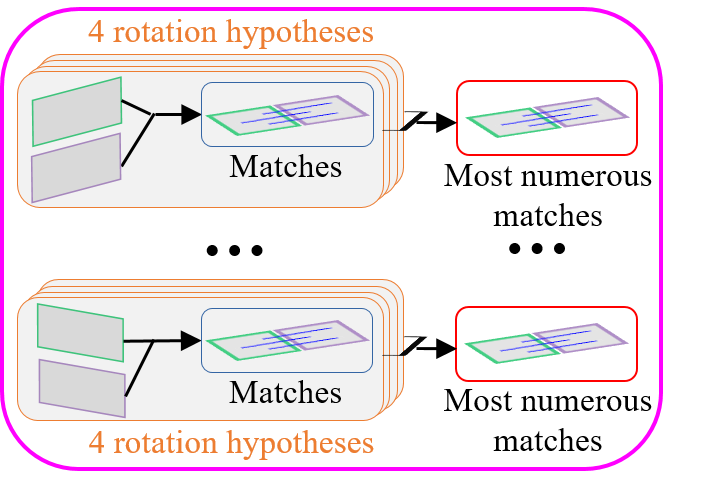
\includegraphics[width=5cm]{images/Chapitre3/R3D-superglue.png}
		\end{minipage}%
	}
        \subfigure[Four rotation hypotheses]{
    \begin{minipage}[t]{0.8\linewidth}
        \centering
        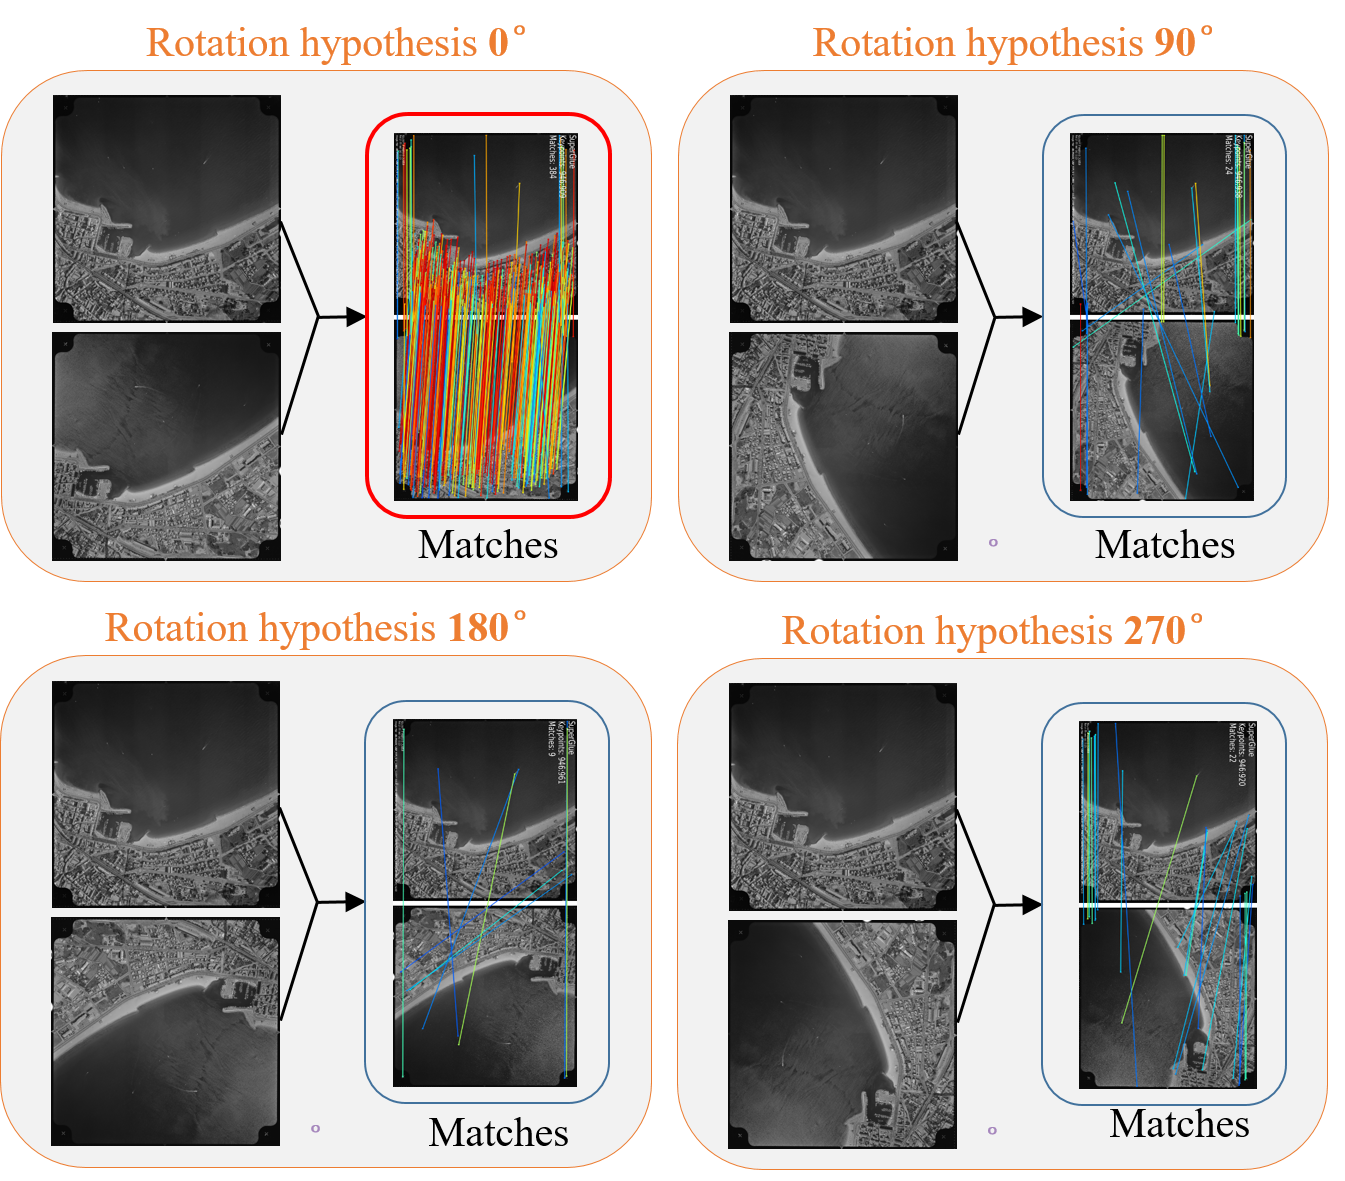
\includegraphics[width=0.8\columnwidth]{images/Chapitre3/R3D-RotHyp.png}
    \end{minipage}%
}
        %\caption{Rough co-registration by matching image pairs. (a) Workflow of \textit{ImgPairs}. Each inter-epoch image pair is matched, followed by projecting the matches onto ground to find globally consistent inliers. (b) Four rotation hypotheses. We rotate the secondary image by 90 $^\circ$ four times to match with master image and keep the best one with the largest number of matches (red rectangle).}
        \caption{Rough co-registration by matching image pairs (i.e., \textit{ImgPairs}). (a) Whole workflow. Each inter-epoch image pair is matched individually, followed by projecting the matches onto ground to find globally consistent inliers. (b) Match image pairs with SIFT, which involves matching followed by 2D similarity RANSAC to find inliers. (c) Match image pairs with SuperGlue, which involves matching combined with \textit{four rotation hypotheses}. (d) Four rotation hypotheses. We rotate the secondary image by 90 $^\circ$ four times to match with master image and keep the best one with the largest number of matches (red rectangle).}
        \label{WorkflowImgPair}
    \end{center}
\end{figure*}

This strategy is adapted from our early attempt to match different epochs by matching P$\times$Q inter-epoch image pairs separately without the later step of building a globally consistent transformation model. \zll{In ~\cite{zhang2020guided} we accomplished it by estimating a 2D similarity model for each image pair and using it to guide precise matching.} Obviously it is less robust as the P$\times$Q 2D similarity models might not be consistent.
%\par
However, the idea of using 2D similarity model to guide matching is more generic as it doesn't require initial orientations $O_{ini}^{e_i}$ and \ac{DSM}s $D_{ini}^{e_i}$. It is a viable and maybe even the only possible approach when it is impossible to acquire orientations $O_{ini}^{e_i}$ and \ac{DSM}s $D_{ini}^{e_i}$. An example is demonstrated in section~\ref{inputHomography}. %Appendix ~\ref{chap:appendix3} 

%helpful in specific cases when the orientations $O_{ini}^{e_i}$ and \ac{DSM}s $D_{ini}^{e_i}$ are not available. This might happen when we don't have stereoscopic configuration  due to difficulty to match intra-epoch image pairs. In Appendix ~\ref{chap:appendix3} we displayed a small dataset over snow-covered area. It consists of only one epoch. However, there are images among them that are extremely challenging to match, both SIFT and SuperGlue failed on it. We provide the option to input a rough 2D similarity transformation model for prediction to narrow down the search space and therefore successfully recovered several good matches.

%\begin{figure*}[htbp]
%    \begin{center}
%        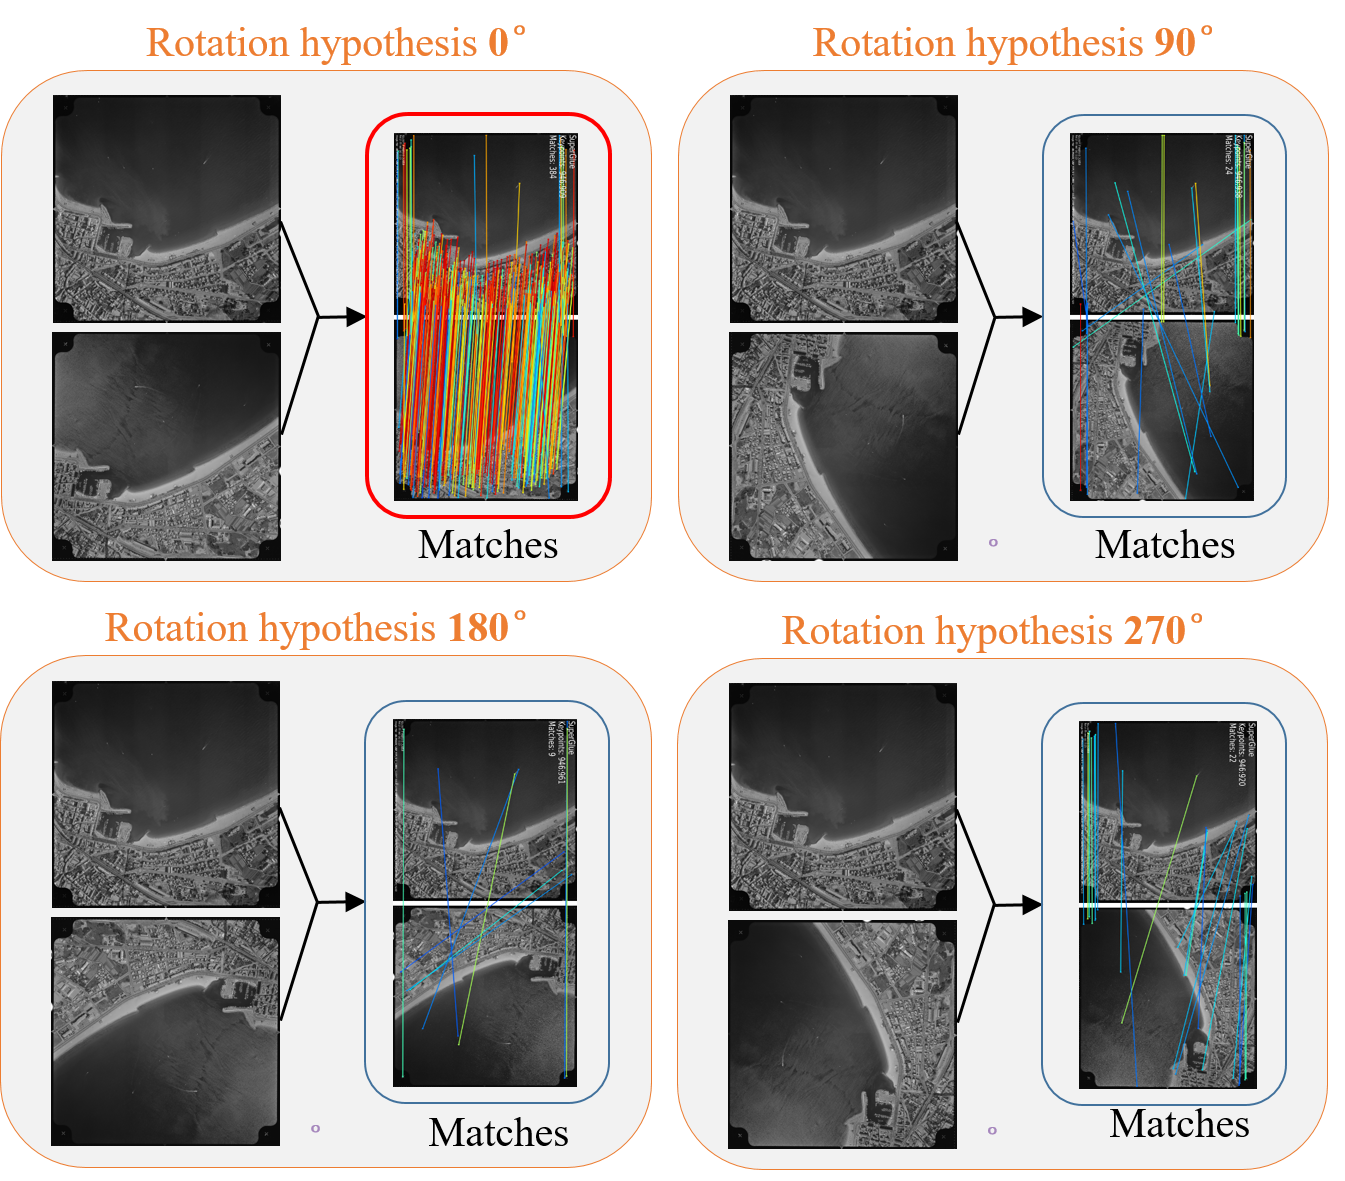
\includegraphics[width=0.8\columnwidth]{images/Chapitre3/R3D-RotHyp.png}
%        \caption{4 rotation hypotheses of matching image pairs.}
%        \label{Flow-process diagram}
%    \end{center}
%\end{figure*}

\subsection{Strategy 2: Matching Orthophotos/DSMs (\textit{Ortho} or \textit{DSM})}
%\subsection{trategy 2: global matching}
Another strategy is to match orthophotos or \ac{DSM}s. %, which is suitable for both aerial images and satellite images. 
The detailed workflows are displayed in Figure~\ref{WorkflowOrtho}(a) and Figure~\ref{WorkflowDSM}(a) individually. Different than matching P$\times$Q image pairs in strategy \textit{ImgPairs}, we only need to match one pair of \ac{DSM}s/orthophotos. 
\zll{The \ac{DSM}s are typically floating-point images, in order to apply feature matching methods directly on them without adjusting the implementation of SIFT or SuperGlue, we further describe the conversion of \ac{DSM} to a gray-scale raster. Additionally, we propose a \textit{one-to-many tiling scheme} to maximize the performance of feature matching with learned methods.}
\begin{figure*}[htbp]
    \begin{center}
        \subfigure[Workflow of \textit{Ortho}]{
            \begin{minipage}[t]{1\linewidth}
                \centering
                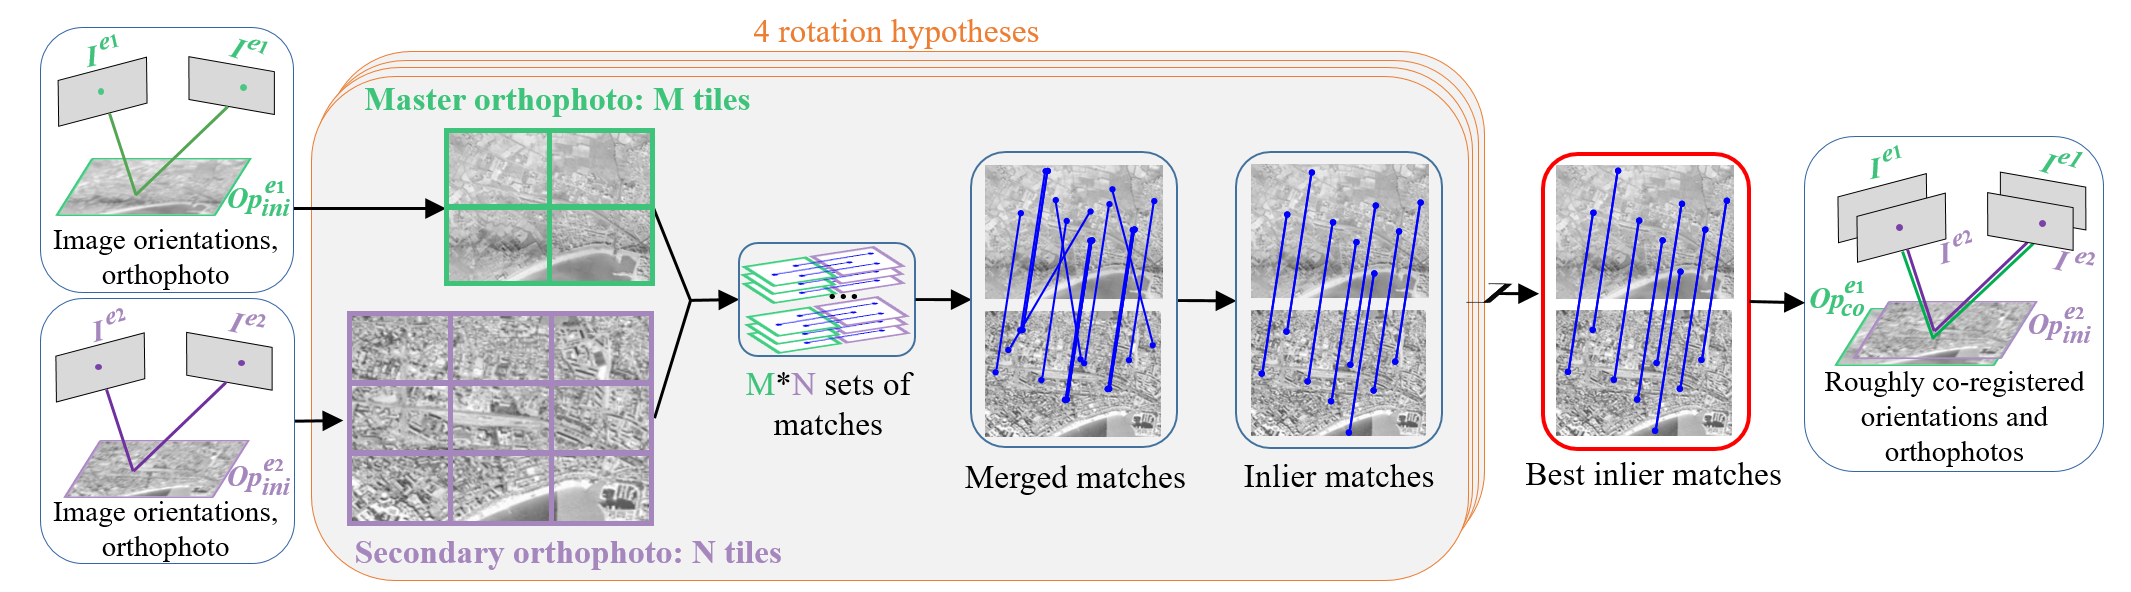
\includegraphics[width=1\columnwidth]{images/Chapitre3/ortho.png}
            \end{minipage}%
        }
        \subfigure[Four rotation hypotheses combined with \textit{one-to-many tiling scheme}]{
            \begin{minipage}[t]{1\linewidth}
                \centering
                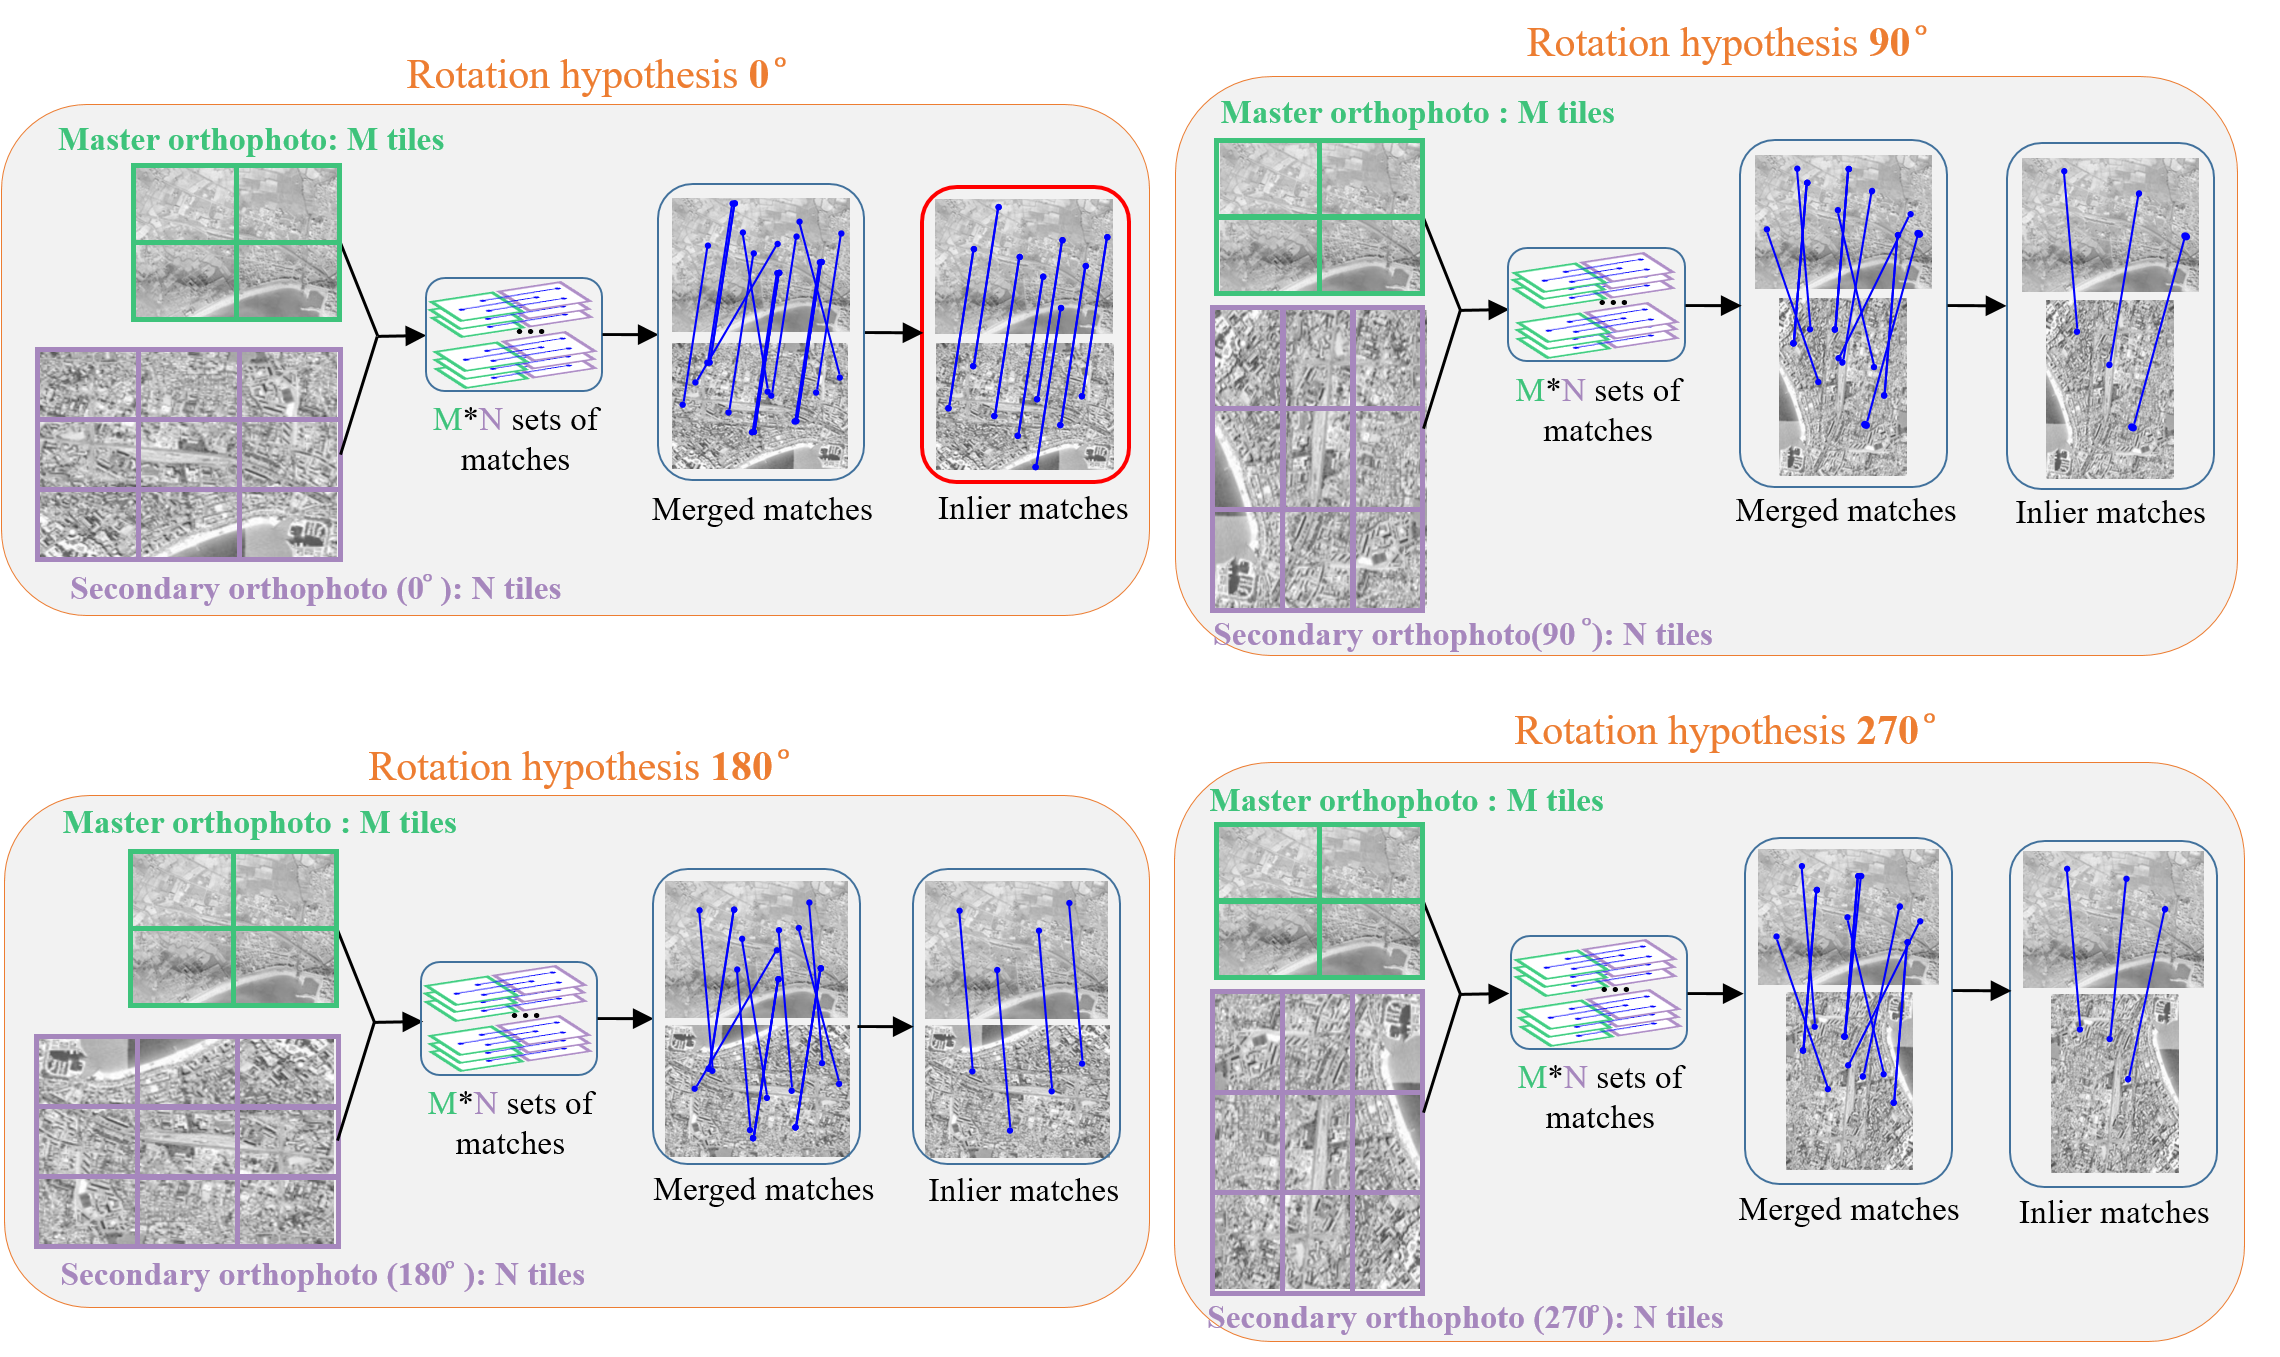
\includegraphics[width=1\columnwidth]{images/Chapitre3/ortho-RotHyp.png}
            \end{minipage}%
        }
        \caption{Rough co-registration by matching orthophotos (i.e., \textit{Ortho}). (a) Whole workflow. Orthophotos are matched, followed by projecting the inlier matches onto ground to build 3D Helmert transformation model. (b) Four rotation hypotheses combined with \textit{one-to-many tiling scheme}. We rotate the secondary orthophoto by 90 $^\circ$ four times to match with master orthophoto and keep the best one with the largest number of RANSAC inliers (red rectangle). \textit{One-to-many tiling scheme} is applied during each hypothesis, with both orthophotos croped into tiles followed by matching all the tile pairs and merging the matches.}
        \label{WorkflowOrtho}
    \end{center}
\end{figure*}

%\begin{figure*}[htbp]
%    \begin{center}
%        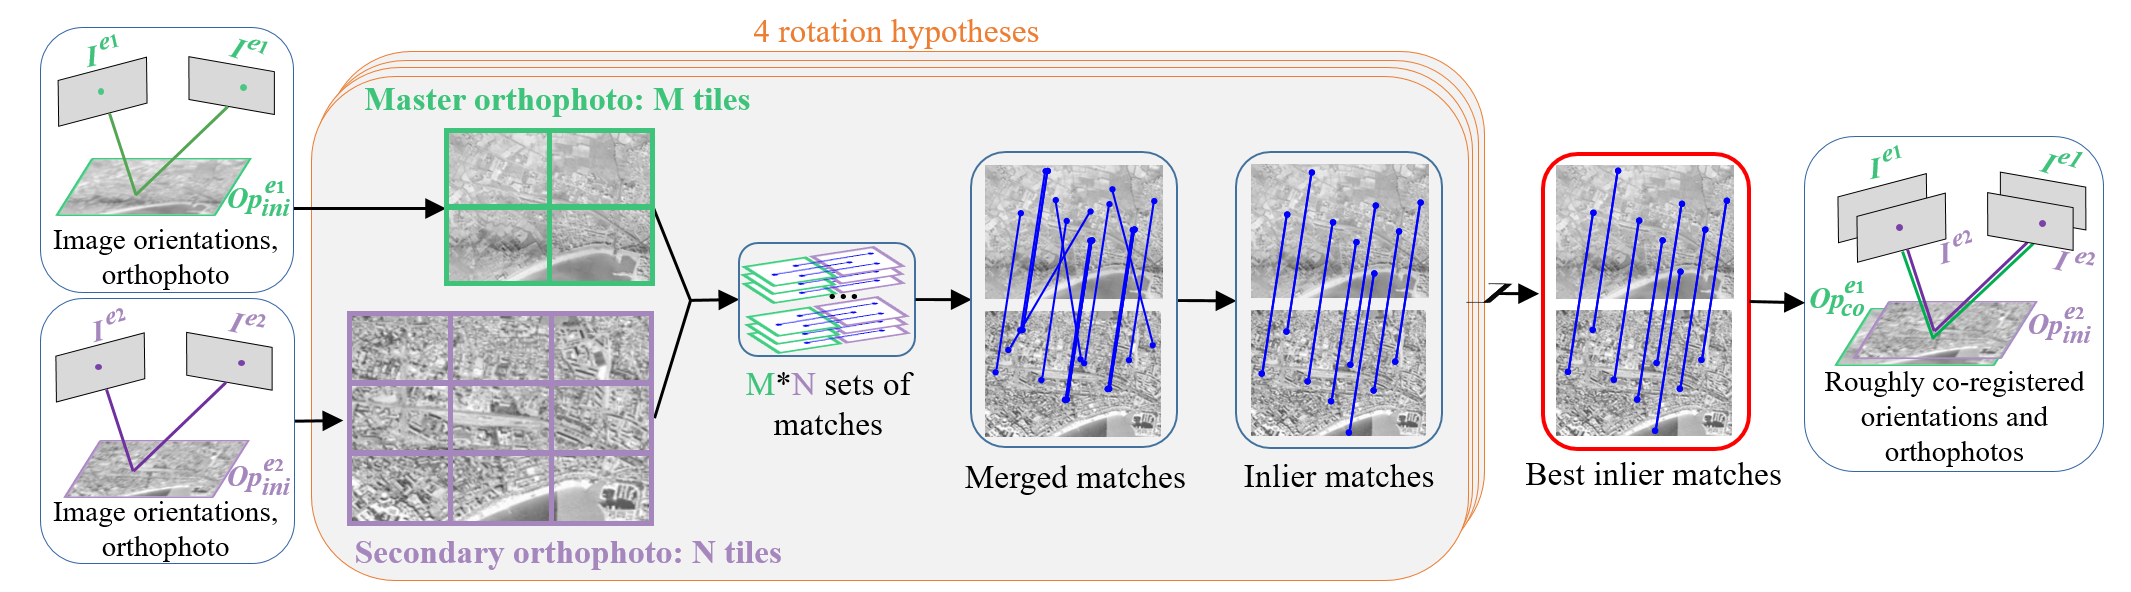
\includegraphics[width=1\columnwidth]{images/Chapitre3/ortho.png}
%        \caption{Rough co-registration by matching orthophotos.}
%        \label{Flow-process diagram}
%    \end{center}
%\end{figure*}
%
%\begin{figure*}[htbp]
%    \begin{center}
%        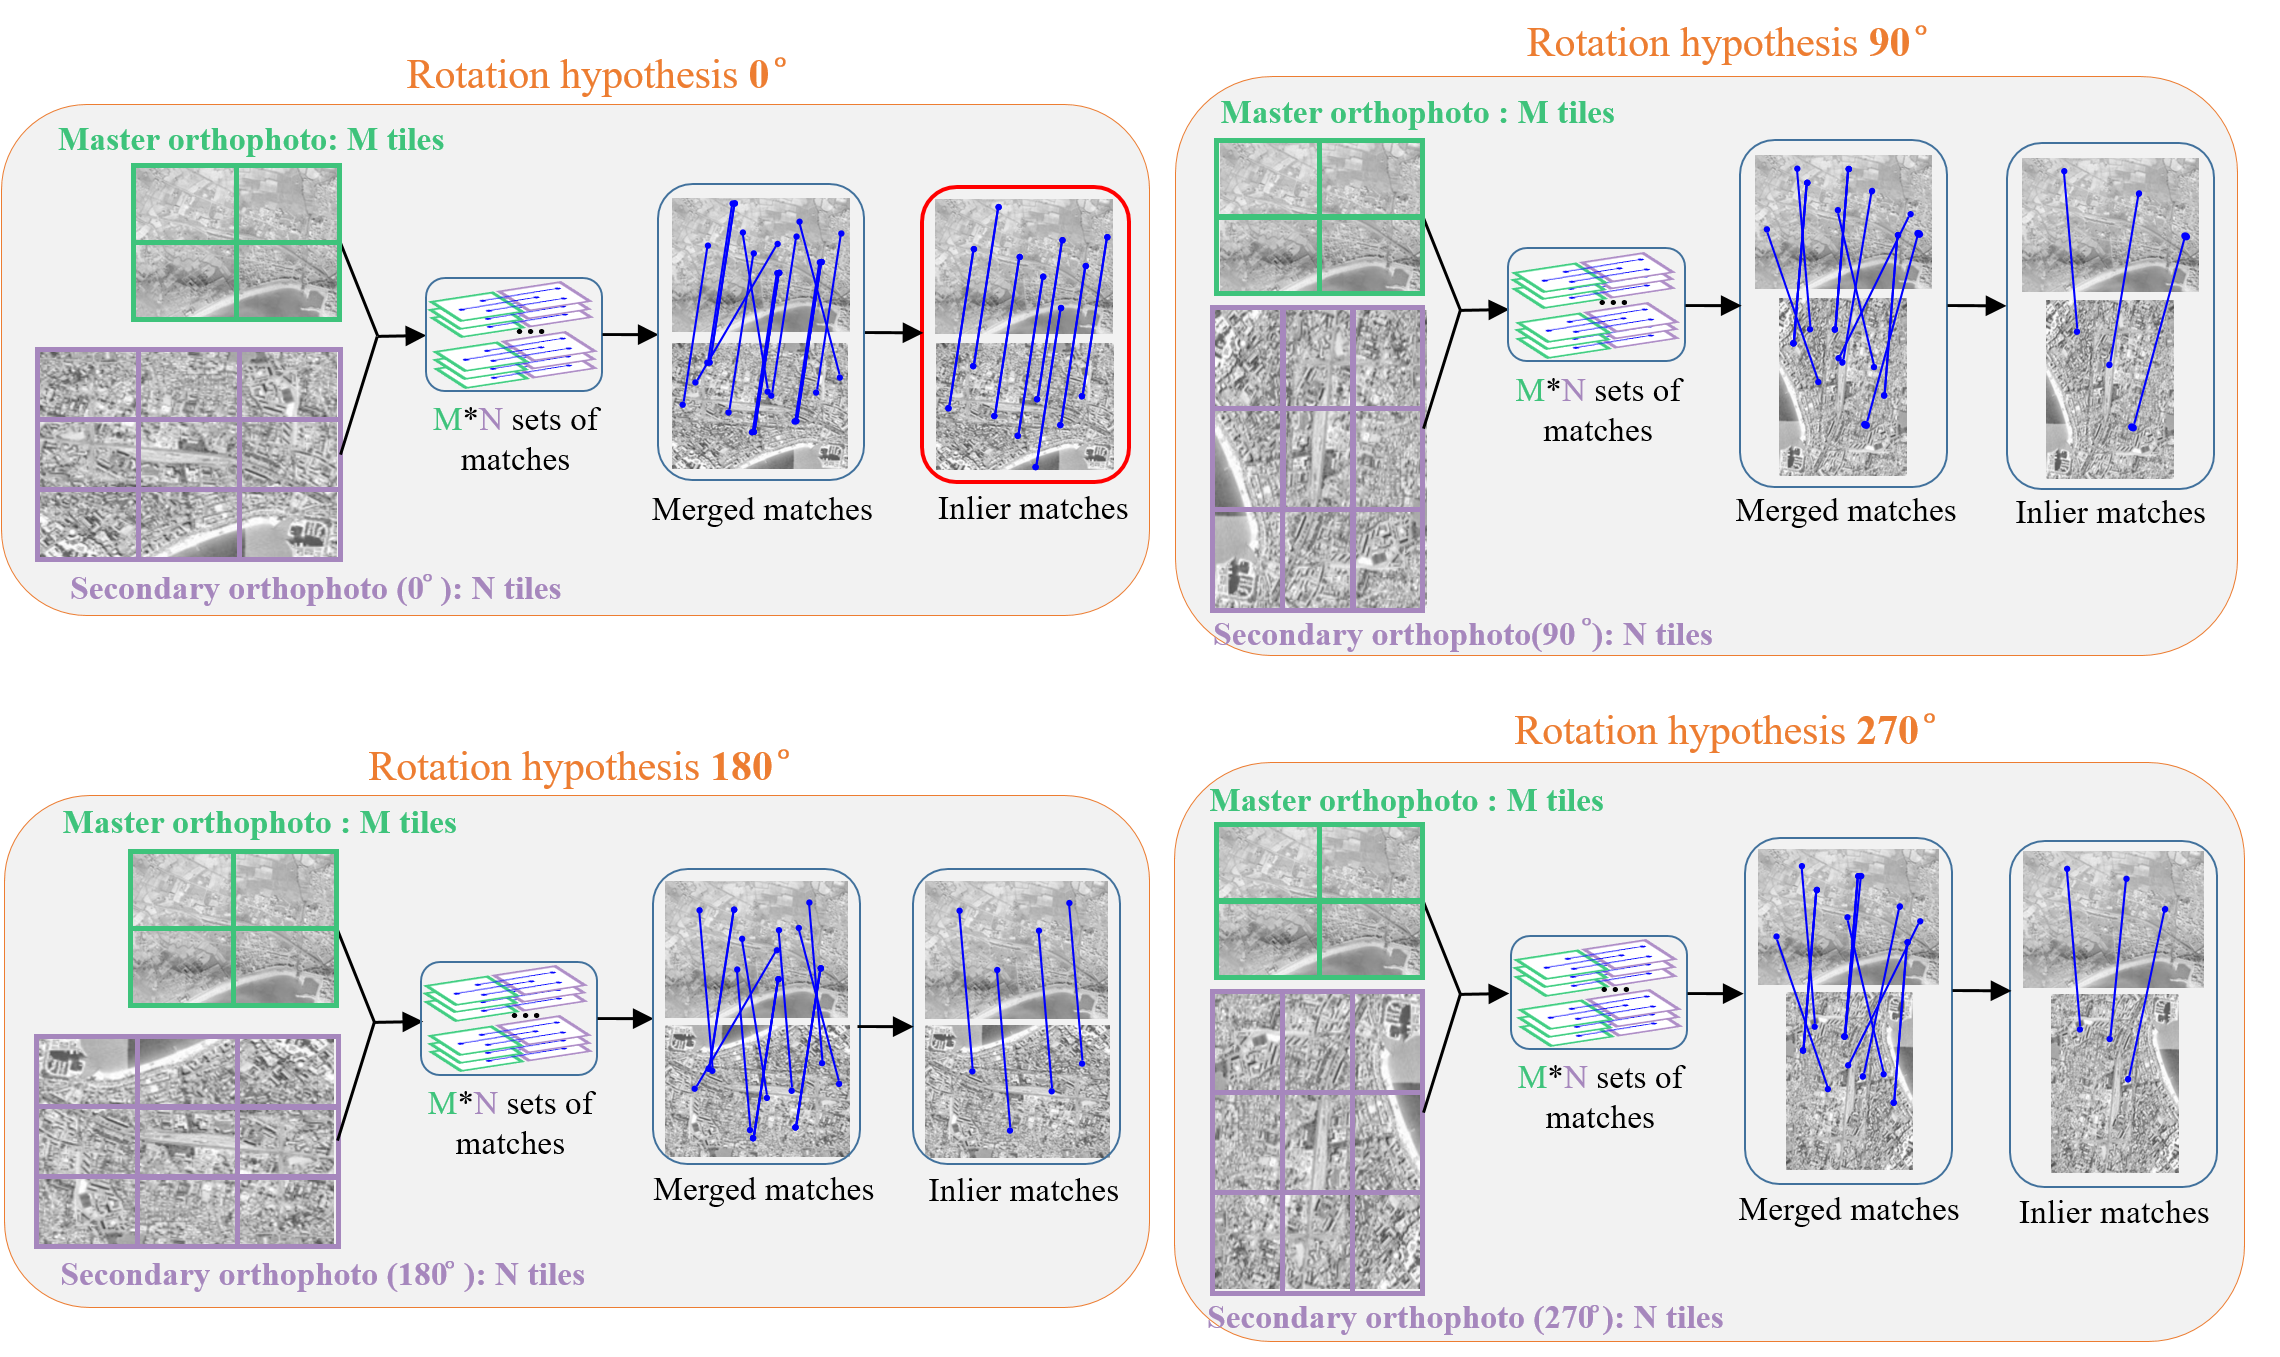
\includegraphics[width=0.8\columnwidth]{images/Chapitre3/ortho-RotHyp.png}
%        \caption{4 rotation hypotheses of matching orthophotos.}
%        \label{Flow-process diagram}
%    \end{center}
%\end{figure*}

%%%%%%%%%%%%%%%%%%%%%%%%%%%%%%

\begin{figure*}[htbp]
    \begin{center}
        \subfigure[Workflow of \textit{DSM}]{
            \begin{minipage}[t]{1\linewidth}
                \centering
                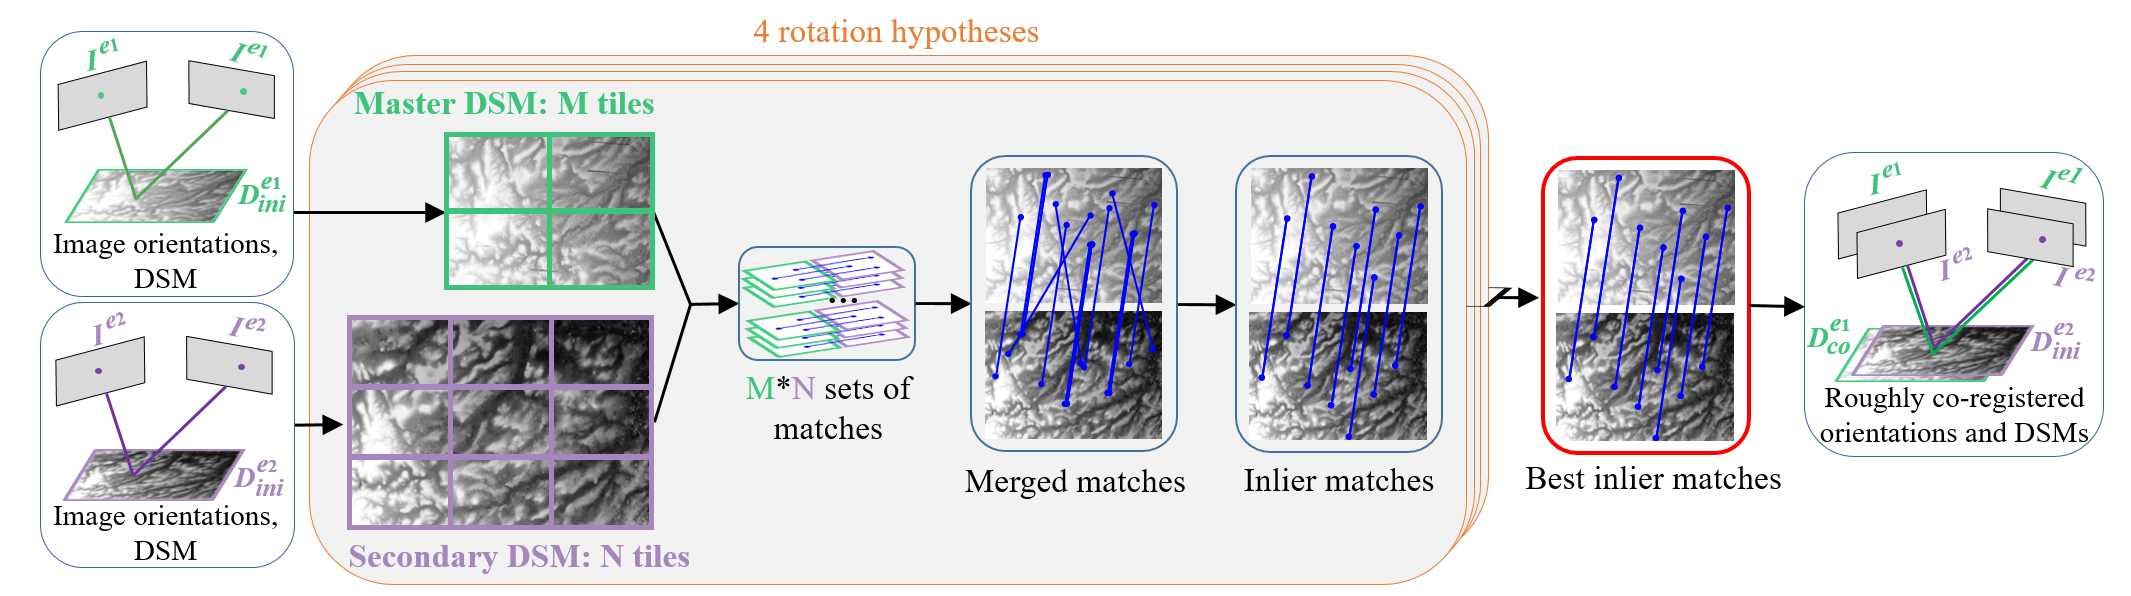
\includegraphics[width=1\columnwidth]{images/Chapitre3/dsm.png}
            \end{minipage}%
        }
        \subfigure[Four rotation hypotheses combined with tiling scheme]{
            \begin{minipage}[t]{1\linewidth}
                \centering
                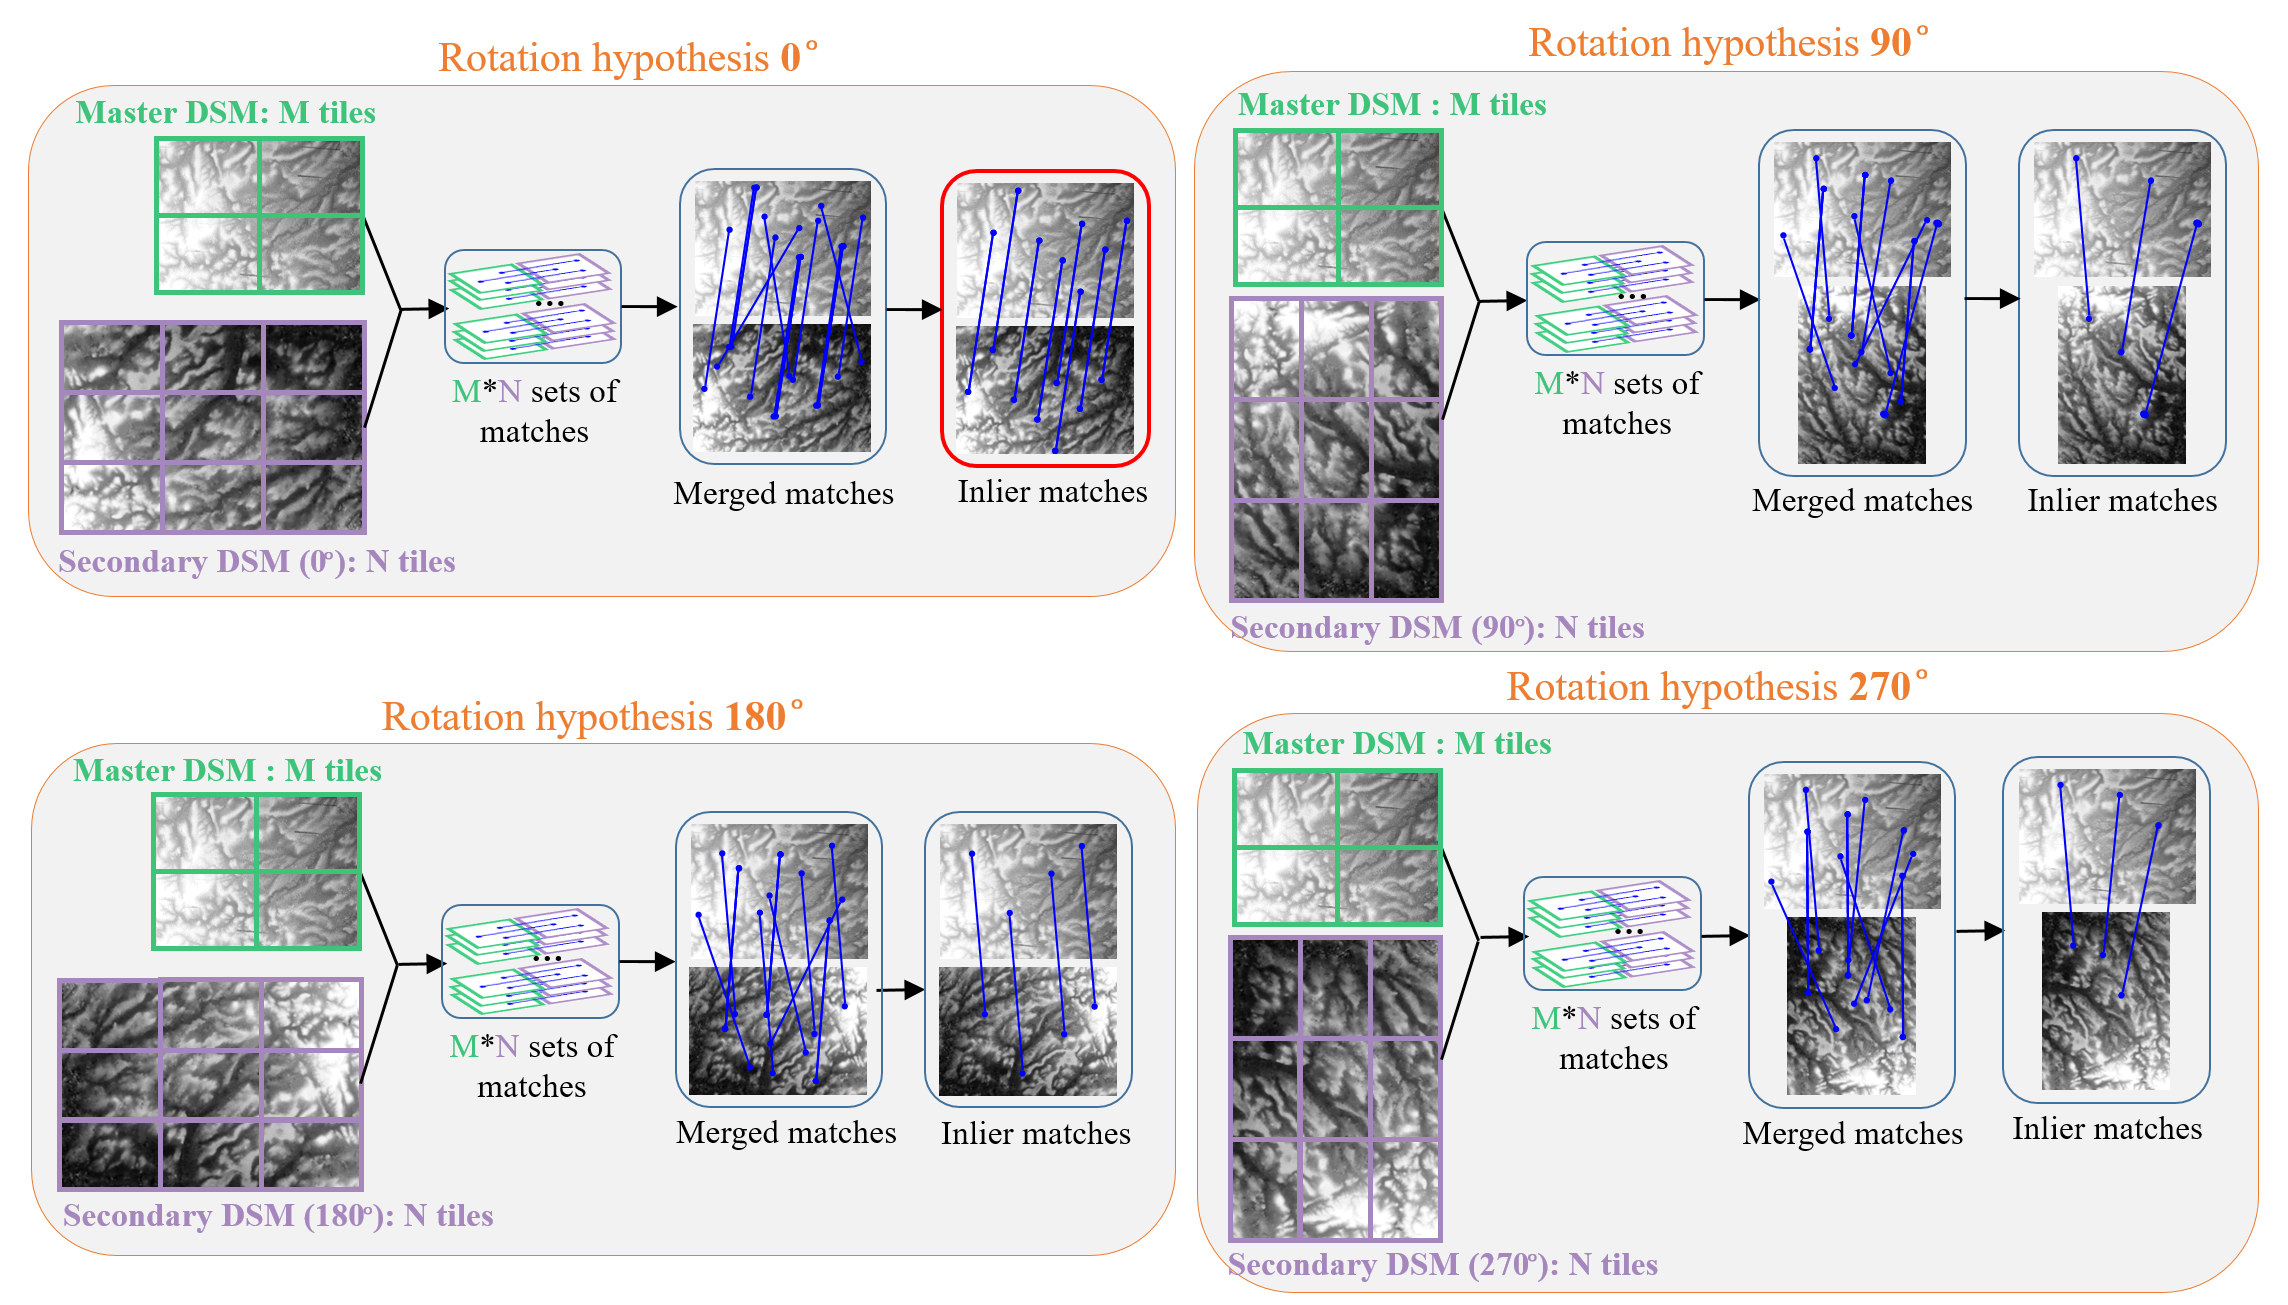
\includegraphics[width=1\columnwidth]{images/Chapitre3/dsm-RotHyp.png}
            \end{minipage}%
        }
        \caption{Rough co-registration by matching \ac{DSM}s (i.e., \textit{DSM}). (a) Whole workflow. \ac{DSM}s are matched, followed by projecting the inlier matches onto ground to build 3D Helmert transformation model. (b) Four rotation hypotheses combined with tiling scheme. We rotate the secondary \ac{DSM} by 90 $^\circ$ four times to match with master \ac{DSM} and keep the best one with the largest number of RANSAC inliers (red rectangle). Tiling scheme is applied during each hypothesis, with both \ac{DSM}s cropped into tiles followed by matching all the tile pairs and merging the matches.}
        \label{WorkflowDSM}
    \end{center}
\end{figure*}

%\begin{figure*}[htbp]
%    \begin{center}
%        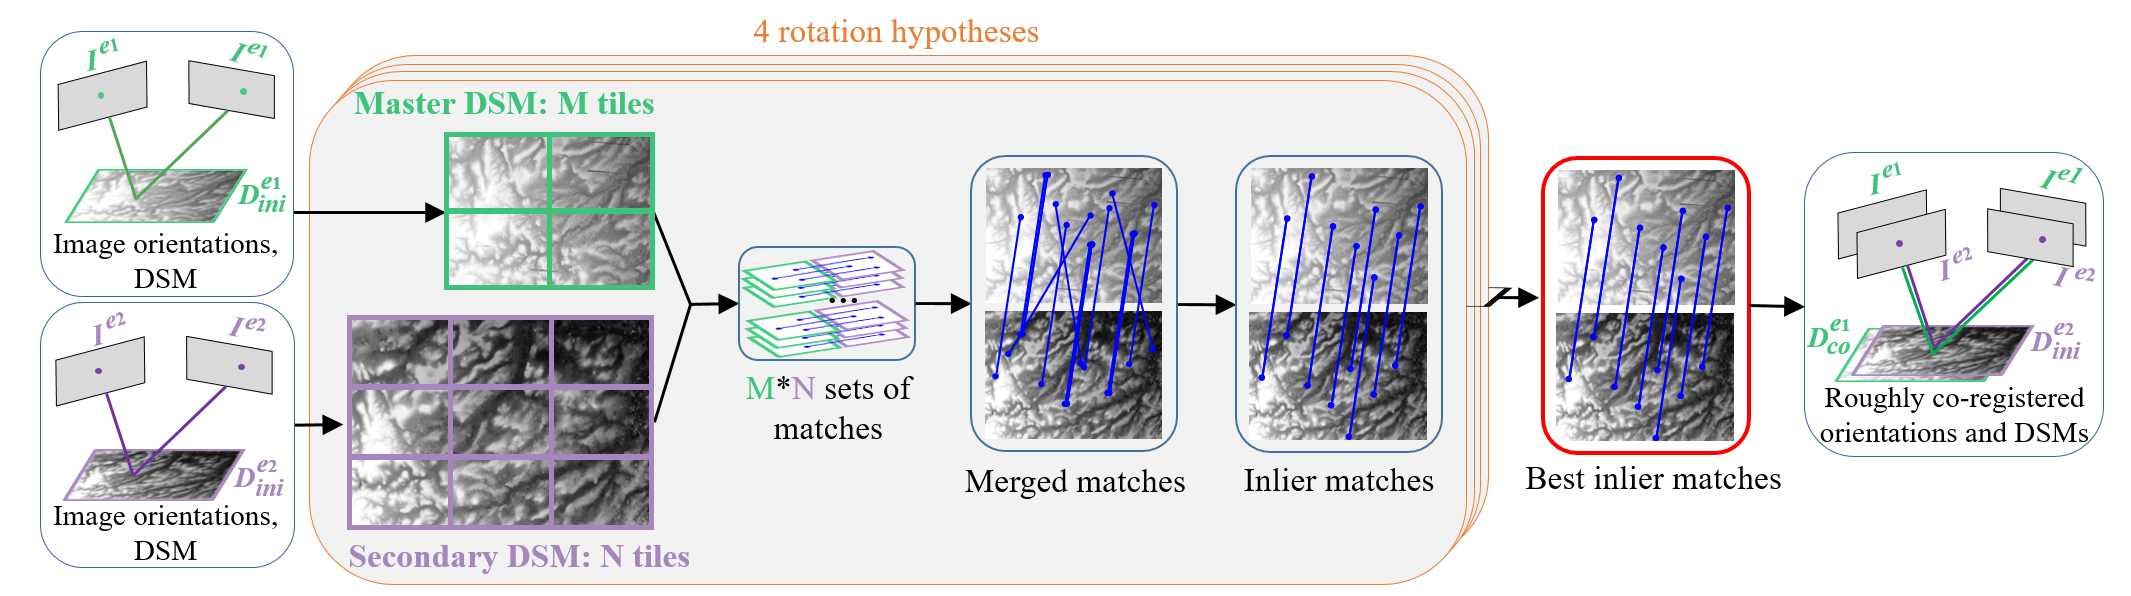
\includegraphics[width=1\columnwidth]{images/Chapitre3/dsm.png}
%        \caption{Rough co-registration by matching DSMs.}
%        \label{Flow-process diagram}
%    \end{center}
%\end{figure*}
%
%\begin{figure*}[htbp]
%    \begin{center}
%        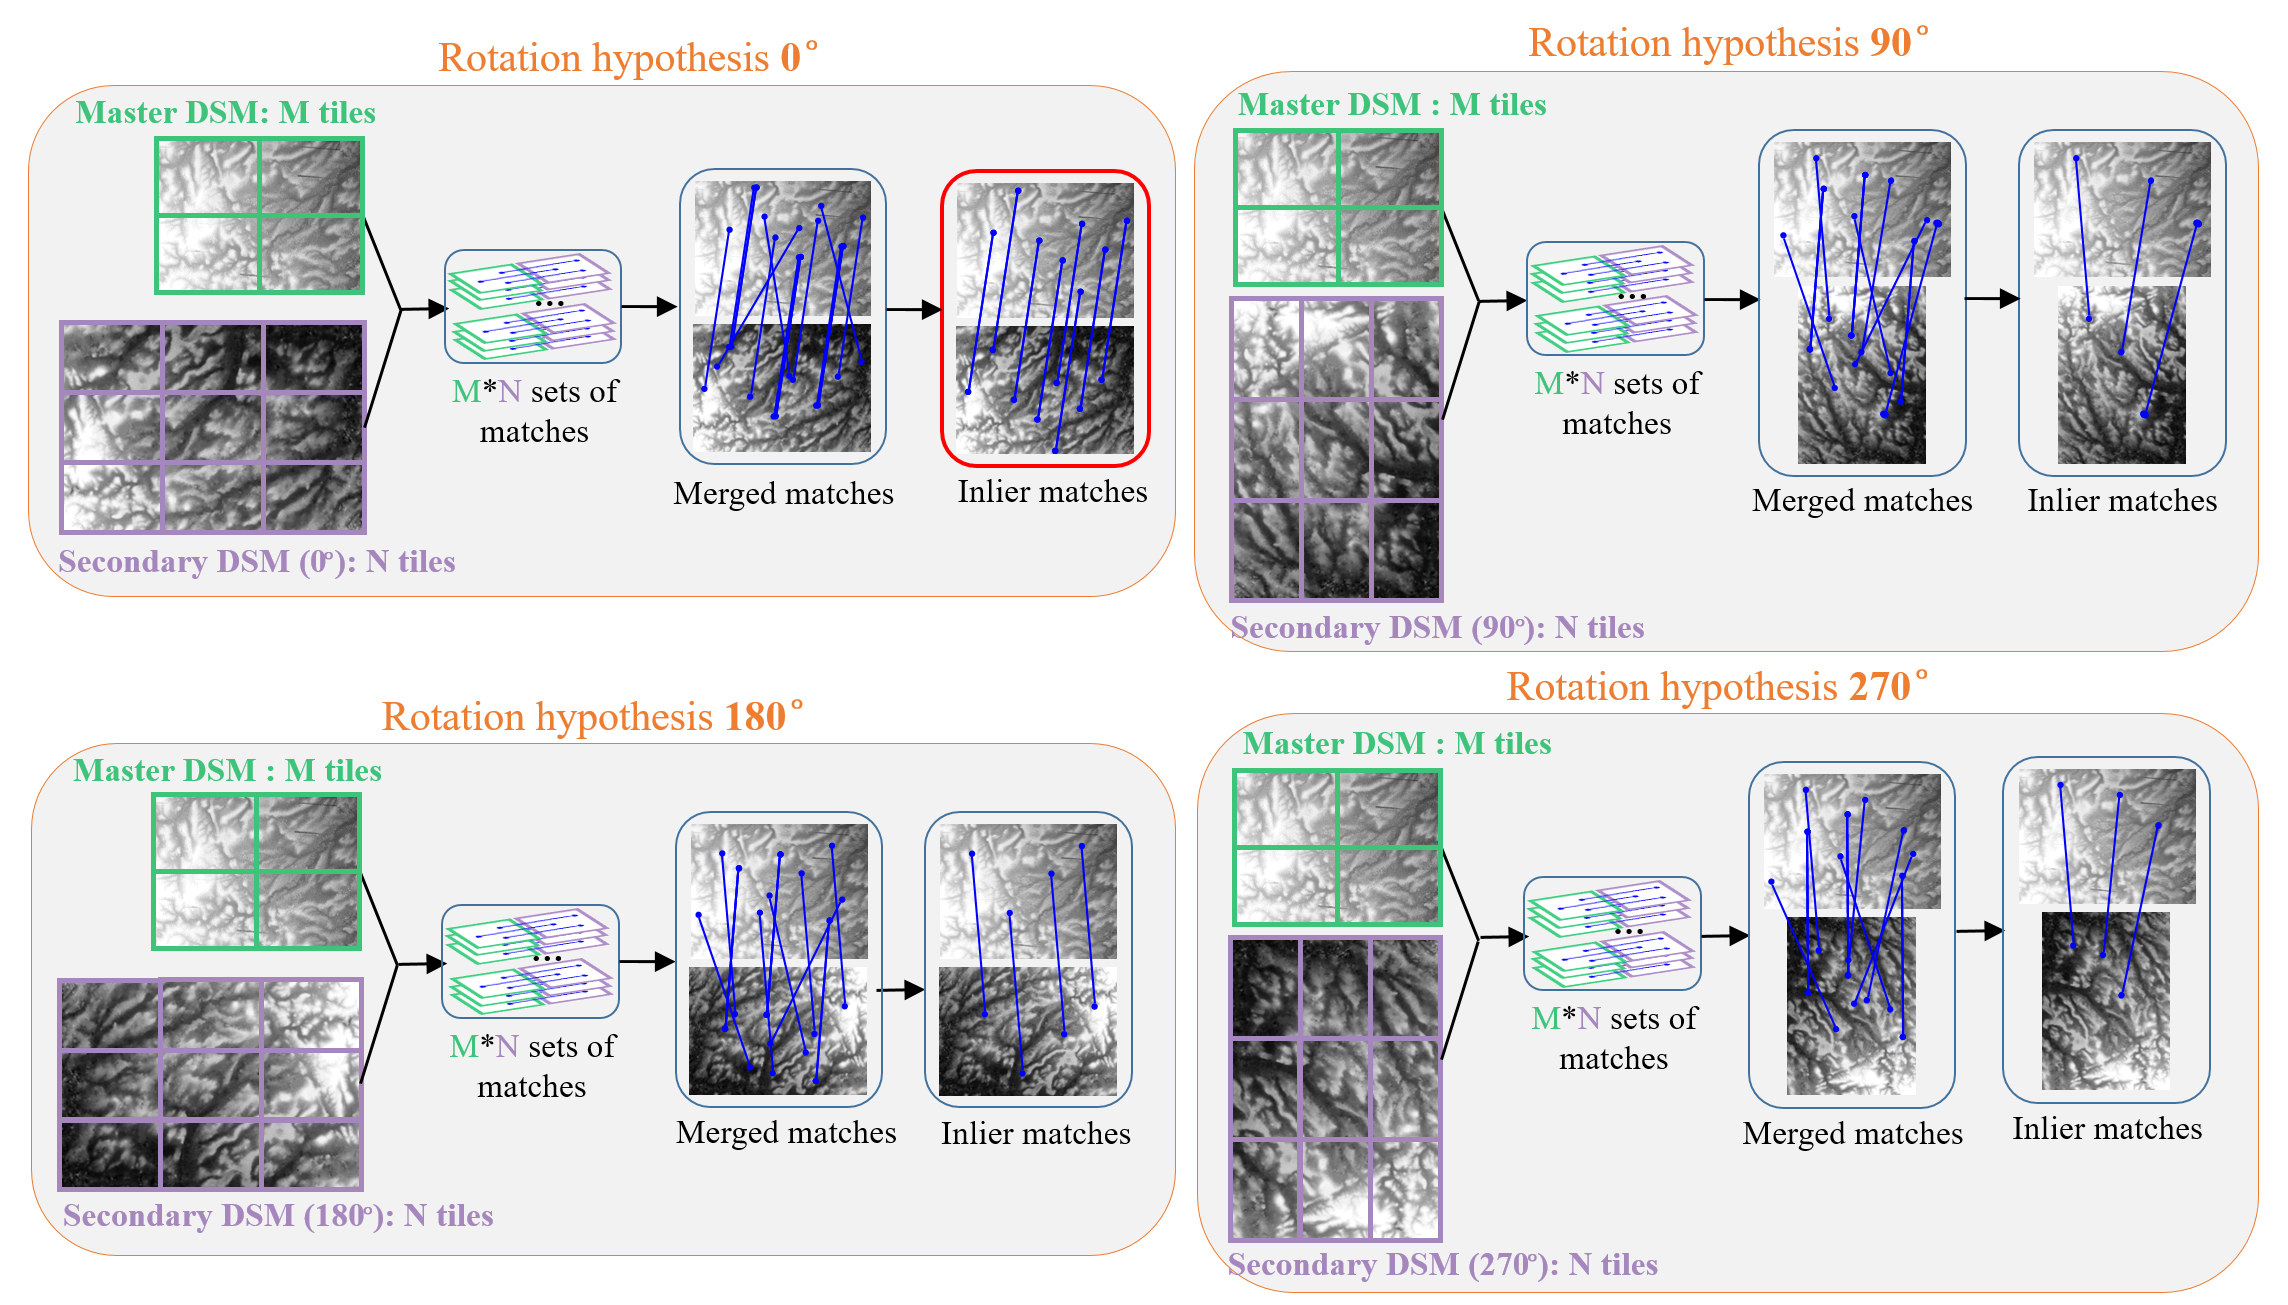
\includegraphics[width=0.8\columnwidth]{images/Chapitre3/dsm-RotHyp.png}
%        \caption{4 rotation hypotheses of matching DSMs.}
%        \label{Flow-process diagram}
%    \end{center}
%\end{figure*}


\par
Matching \ac{DSM}s/orthophotos has the following merits: (1) redundancy caused by the forward and side overlapping areas is removed; (2) it enables a follow-up search for globally consistent inliers directly without the need to project matches onto ground; (3) it decreases the combinatorial complexity caused by rotation ambiguity of P$\times$Q images; (4) when matching \ac{DSM}s, robust matches can be expected even under extreme scene changes, as 3D landscape generally provide stable information over time.\\
\paragraph{Converting \ac{DSM} to grayscale image.} %Orthophotos are by nature RGB images, therefore
\ac{DSM}s are 2.5D rasters recorded in floating-point format. It is complicated to apply feature matching methods on them directly, as most of the methods are implemented for RGB images. Therefore, we convert \ac{DSM} beforehand to [0–255] range grayscale images as follows:\\
\begin{enumerate}
	\item Calculate the standard deviation of the \ac{DSM} elevation;
	\item Pixels with elevations larger than double the standard deviation are considered outliers and therefore ignored;
	\item Transform the inlier pixels to the range of [0-255], resulting in grayscale image.
	\item Apply Wallis filter on the grayscale image to get rid of uneven illumination, resulting in more informative image.
\end{enumerate}

\paragraph{\textit{One-to-many tiling scheme}.}
\ac{DSM}s/orthophotos are usually large images as they have larger extent than original images.
Learned matching methods often underperform on large images as they are either trained on small images in order to run real-time or with limited spatial resolution of \ac{CNN} feature maps. To make up for the deficiency, we propose an \textit{one-to-many tiling scheme}, which is performed as follows (Figure~\ref{WorkflowOrtho}(a) and Figure~\ref{WorkflowDSM}(a)):\\
\begin{enumerate}
    \item Crop master and secondary images into M and N tiles of size $SZ_{one-to-many}$; %(1280$\times$960 pixels in our experiments);
    \item Apply matching on M$\times$N tile pairs respectively;
    \item Merge the matches and perform RANSAC based on 2D similarity transformation to remove outliers.
\end{enumerate}                                   
%In order to demonstrate if the \textit{one-to-many tiling scheme} helps, in section~\ref{Compare2SpGs} %Appendix ~\ref{chap:appendix2} 
%we compared 2 sets of the results on matching multi-epoch orthophotos and DSMs: (1) $SuperGlue_{orig}$: SuperGlue without our \textit{one-to-many tiling scheme}; (2) $SuperGlue_{tiling}$: SuperGlue combined with our \textit{one-to-many tiling scheme}. As can be seen, $SuperGlue_{orig}$ failed while $SuperGlue_{tiling}$ recovered a large number of good matches.
\par
The \textit{one-to-many tiling scheme} can be combined with \textit{4 rotation hypotheses}, as shown in Figure~\ref{WorkflowOrtho}(b) and Figure~\ref{WorkflowDSM}(b).
%Both \textit{one-to-many tiling scheme} and \textit{4 rotation hypotheses} would not be applied when matching method that is satisfactory on large images and rotation invariant (e.g., SIFT) is adopted.
\paragraph{Workflow of \textit{Ortho} and \textit{DSM}.} 
The matching \ac{DSM}s/orthophotos strategy works as follows:\\
\begin{enumerate}
    \item Transform \ac{DSM}s to grayscale images if the strategy \textit{DSM} is applied.
    \item Match \ac{DSM}s/orthophotos, giving rise to one set of matches $M({\mathbf{K}^{e_1},\mathbf{K}^{e_2}})$ ($\mathbf{K}^{e_i}$ represents keypoints in \ac{DSM} $D^{e_i}$ or orthophoto $Op^{e_i}$).
    %\item Run RANSAC on matches based on 2D similarity transformation model to remove outliers.
    \item Sample matches $M({\mathbf{K}^{e_1},\mathbf{K}^{e_2}})$ iteratively to compute the 2D similarity transformation RANSAC model:
\begin{equation}
\left [ \begin{array}{c}
{K}_x^{e_2}\\
{K}_y^{e_2}
\end{array}
\right ] =\lambda \cdot { \left[ \begin{array}{cc}
    cos\theta & sin\theta\\
    -sin\theta & cos\theta
    \end{array} 
    \right ]} \cdot {\left [ \begin{array}{c}
    {K}_x^{e_1}\\
    {K}_y^{e_1}
    \end{array}
    \right ]} + \left [ \begin{array}{c}
\Delta_x\\
\Delta_y
\end{array}
\right ]. \label{eq:2DSim}
\end{equation}

%   \begin{equation*}
%       {KG_i^{e_2}} = \lambda \cdot \mathbf{R} \cdot {KG_i^{e_1}} + \mathbf{T} , \quad i \in [1,3] \label{eq:3Dsim}
%   \end{equation*}
    where $\lambda$ is the scale factor, $\theta$ is the in-plane rotation angle and $\left [ \begin{array}{c}
    \Delta_x, \Delta_y
    \end{array}
    \right ]$ $^{^T}$ is the translation vector.
    %$\mathbf{T}$ is the translation vector and $\mathbf{R}$ is the rotation matrix.
    \zll{Matches within $T_r$ of its predicted position (i.e., $\lvert \mathbf{K}^{e_2} - (\lambda \cdot {\left[ \begin{array}{cc}
    	cos\theta & sin\theta\\
    	-sin\theta & cos\theta
    	\end{array} 
    	\right]} \cdot \mathbf{K}^{e_1} + \Delta) \rvert < T_r$) are considered as inliers.}    
    %We set the number of RANSAC iterations to 1000, and consider matches within $T_r$ of its predicted position as inliers. In our experiment, {$T_r$ was set to 15 pixels.}
    \item Project the inlier matches onto \ac{DSM} $D_{ini}^{e_i}$ to fit the best 3D Helmert transformation parameters.
\end{enumerate}

\section{Experiments}
As described in the previous section, we provide 3 pipelines out of 2 strategies to perform rough co-registration:\\
\begin{enumerate}
	\item \textit{ImgPairs}: match image pairs;
	\item \textit{Ortho}: match orthophotos;
	\item \textit{DSM}: match \ac{DSM}s.
\end{enumerate}
%\begin{enumerate}
%    \item Match image pairs: hereinafter referred to as \textit{ImgPairs};
%    \item Match orthophotos: hereinafter referred to as \textit{Ortho};
%    \item Match \ac{DSM}s: hereinafter referred to as \textit{DSM}.
%\end{enumerate}
For each pipeline, we employ either SIFT or SuperGlue as the feature matching method, giving rise to 6 variants:\\
\begin{enumerate}
    \item $SIFT_{ImgPairs}$;
    \item $SuperGlue_{ImgPairs}$;
    \item $SIFT_{Ortho}$;
    \item $SuperGlue_{Ortho}$;
    \item $SIFT_{DSM}$;
    \item $SuperGlue_{DSM}$;
\end{enumerate}
We test the 6 variants on all the multi-epoch datasets which are elaborated in Chapter~\ref{chap:ApplicationsAndDatasets}: Fr{\'e}jus, Pezenas, Kobe and Alberona, except that we skip the variants $SIFT_{ImgPairs}$ and $SuperGlue_{ImgPairs}$ for satellite images in Pezenas as there are only 2 images with the same extent.\\

\zll{Additionally, we provide experiments where we test the influence of the SIFT parameters (image downsampling factor, ratio test, RANSAC, etc.) in Section \ref{Compare2SIFTs} and the effectiveness of \textit{one-to-many tiling scheme} in Section~\ref{Compare2SpGs}. In Section \ref{inputHomography} we demonstrate a real case study where the basic 2D similarity model outperforms the more sophisticated 3D Helmert transformation model. Finally, the 6 variants are compared in Section \ref{Comparisonof6variants}.\\}

%As inter-epoch images often look very different, when the original SIFT ~\cite{lowe2004distinctive} (i.e., $SIFT_{Default}$) is applied directly in our methods $SIFT_{ImgPairs}$, $SIFT_{Ortho}$ and $SIFT_{DSM}$, generally very few matches are recovered. So we replace it with a slightly different version of SIFT (i.e.,  $SIFT_{Adapted}$) with the following modifications:\\

%For SIFT applied in variants $SIFT_{ImgPairs}$, $SIFT_{Ortho}$ and $SIFT_{DSM}$, we did a test to compare the performance of SIFT with different parameters in Section \ref{Compare2SIFTs}. \\
%For SuperGlue applied in variants $SuperGlue_{ImgPairs}$, $SuperGlue_{Ortho}$ and $SuperGlue_{DSM}$, we did a test in Section~\ref{Compare2SpGs} to demonstrate if the \textit{one-to-many tiling scheme} helps. \\
%Besides, a test of matching a snow-covered intra-epoch image pair is given in Section \ref{inputHomography} to show the strength of using 2D similarity model to guide matching.\\
%Finally, the comparison between 6 variants of our rough co-registration pipeline on 4 sets of multi-epoch datasets are given in Section \ref{Comparisonof6variants}.\\

%In order to demonstrate if the \textit{one-to-many tiling scheme} helps, in section~\ref{Compare2SpGs} %Appendix ~\ref{chap:appendix2} 
%we compared 2 sets of the results on matching multi-epoch orthophotos and DSMs: (1) $SuperGlue_{orig}$: SuperGlue without our \textit{one-to-many tiling scheme}; (2) $SuperGlue_{tiling}$: SuperGlue combined with our \textit{one-to-many tiling scheme}. As can be seen, $SuperGlue_{orig}$ failed while $SuperGlue_{tiling}$ recovered a large number of good matches.

%In the following we give the implementation details, the comparison of SIFT parameters, as well as comparison of the 6 variants.\\



%\subsection{Datasets}
%\label{Datasets}
%%Frejus, Pezenas, Kobe\\
%We tested our rough co-registration variants on all the multi-epoch datasets which are elaborated in Chapter~\ref{chap:ApplicationsAndDatasets}: Fr{\'e}jus, Pezenas, Kobe and Alberona.

%####################################Start Dataset
%Details of the datasets are listed in Table~\ref{AerialData}, ~\ref{SatelliteData} and Figure~\ref{FrejusData},~\ref{PezenasData}, ~\ref{KobeData}.
%\par
%\paragraph{Fr{\'e}jus} It is a 15 $km^2$ rectangular area located in Fr{\'e}jus, a commune in southeastern France. The area is mainly covered with buildings along with scattered farmlands, except a half-moon-shaped bay located in south. We have four sets of aerial images acquired in 1954, 1966, 1970 and 2014. The epoch 2014 was acquired with the \ac{IGN}'s digital metric camera ~\cite{souchon2010ign}, its orientations are both in global reference frame and precise. Therefore it is treated as \ac{GT} during our processing (in other words, the epoch 2014 is chosen as the reference epoch). 
%The area exhibits drastic scene changes in the 60-year period, as can be seen in Figure~\ref{FrejusEvolution}, where evolution of a subregion is displayed.\\
%\paragraph{Pezenas} It is a 420 $km^2$ rectangular area located in Pezenas in the Occitanie region in southern France. The area is mainly covered with vegetation and several sparsely populated urban zones. We have at our disposal three sets of aerial images acquired in 1971, 1981 and 2015, and one set of satellite images acquired in 2014. Both the epoch 2014 and 2015 are treated as \ac{GT}. In this dataset we are interested in matching historical epochs (1971 and 1981) with aerial \ac{GT} and satellite \ac{GT} individually. The area exhibits changes in scene appearance in the 44-year period.\\
%\paragraph{Kobe} It is a 90 $km^2$ area of irregular shape located in the north of Awaji Island, Japan. The well-known Kobe earthquake happened here in January 1995. We have two sets of aerial images: pre-event acquired in 1991 and post-event acquired in 1995. It is mainly covered with mountain area and narrow urban zones along the sea. There is no \ac{GT}, hence we chose the latter epoch (i.e., epoch 1995) as the reference epoch and measured 2 points on Google map to scale the result to metric units. In this dataset we are interested in localizing the earthquake fault.
%
%\paragraph{Alberona} It is a 90 $km^2$ rectangular area located in Southern Italy, near the village of
%Alberona (Puglia region). This portion of the Italian Apennines
%is characterized by the diffuse presence of clay rich lithologies
%which confers to the landscape a typical smooth topography,
%with the wide presence of slow moving landslides of the slide
%and slide-earthflow type. In the study area, the land use is
%typical of rural areas, poorly inhabited and mainly agricultural
%and wooded. A slow
%moving slide-earthflow has been detected there since the 1950s. 
%
%
%\begin{table}[htbp]
%    \scriptsize %\footnotesize
%    \centering
%    \begin{tabular}{||l|c|c|c|c||c|c|c|c||c|c||}\hline
%        &\multicolumn{4}{c||}{Fr{\'e}jus}&\multicolumn{4}{c||}{Pezenas}&\multicolumn{2}{c||}{Kobe}\\\hline
%                &E1954&E1966&E1970&E2014&E1971&E1981&\multicolumn{2}{c||}{E2015}&E1991&E1995\\\hline\hline
%        F [pix]&23350&10230&10230&\color{black}18281&7589&7607&9967.5&9204.5&7662&7662\\
%        %Size [mm]&\color{black}300,300&\color{black}180,180&\color{black}180,180&99.28,72.42&230230&230230&47,35&50,36&212212&212,212\\
%        Wid [mm]&300&180&180&99.28&230&230&47&50&212&212\\
%        Hei [mm]&300&180&180&72.42&230&230&35&36&212&212\\
%        GSD [m]&\color{black}0.11&\color{black}0.17&0.17&0.35&0.32&0.59&0.46&0.5&0.5&0.18\\
%        F. o.&60\%&60\%&60\%&60\%&   60\%&60\%&60\%&60\%&   65\%&65\%\\
%        S. o.&20\%&30\%&30\%&30\%&   20\%&20\%&50\%&50\%&   35\%&65\%\\
%        H  [m]&2500&1700&1700&6500&2400&4500&4600&4600&3800&1400\\
%        Nb &19&15&19&33&57&27&308&74&15&83\\\hline
%    \end{tabular}
%    \caption{Aerial dataset details of Fr{\'e}jus, Pezenas and Kobe. The 2015 acquisition of Pezenas is obtained with two sets of camera. E stands for epoch, F means focal length, Wid and Hei are the width and height of image, GSD is the ground sampling distance, F.o. and S.o. are forward and side overlap, H is the flying height, Nb is the number of images.}
%    \label{AerialData}
%\end{table}
%
%\begin{table}[htbp]
%	\scriptsize %\footnotesize
%	\centering
%	\begin{tabular}{||l|c|c||}\hline
%		& Master image & Secondary image\\\hline
%		Constellation & Pleiades & Pleiades \\
%		GSD [m] & 0.5 & 0.5\\
%		Acquired date & 12/06/2014 & 12/06/2014 \\
%		Number of lines & 38468 & 37710 \\
%		Number of pixels per line & 34108 & 33392 \\
%		Cloud cover & 3.9\% & 4.0\% \\
%		Snow cover & 0\% & 0\% \\\hline
%		%B/H?
%	\end{tabular}
%	\caption{Satellite dataset details of Pezenas. GSD means the ground sampling distance.}
%	\label{SatelliteData}
%\end{table}
%
%\begin{figure*}[htbp]
%    \begin{center}
%        \subfigure[Fr{\'e}jus 1954 (19 images)]{
%            \begin{minipage}[t]{0.4\linewidth}
%                \centering
%                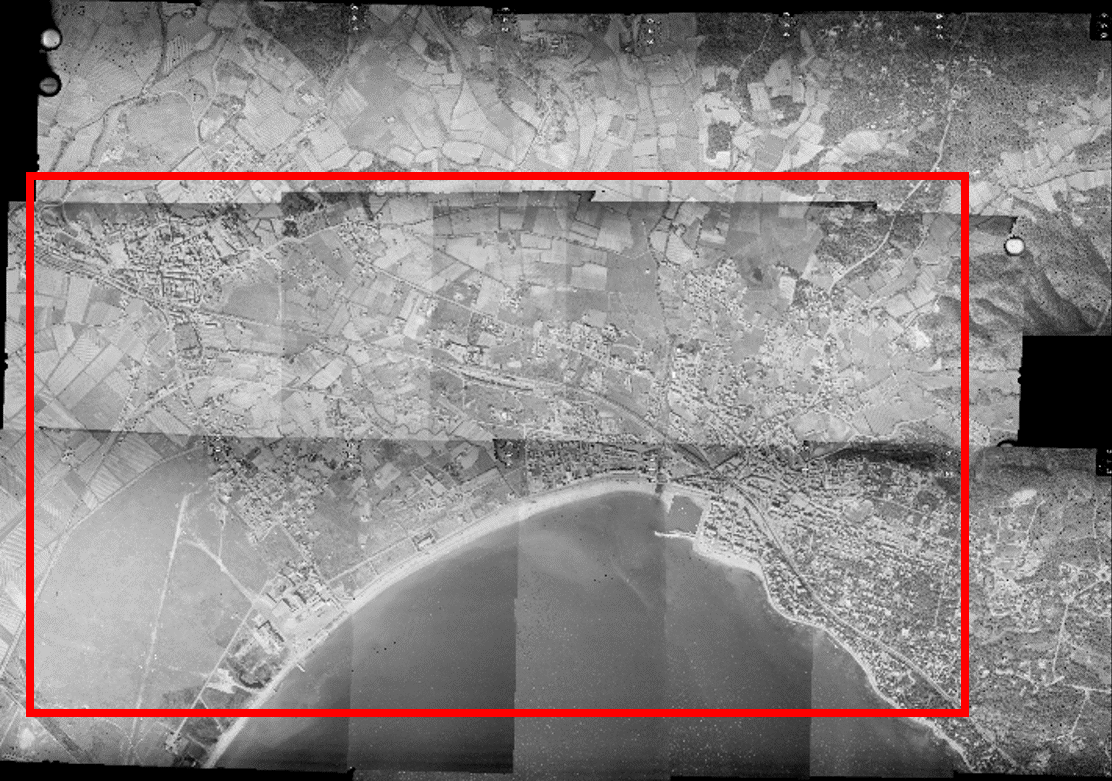
\includegraphics[width=5.65cm]{images/Chapitre3/Frejus1954.png}
%            \end{minipage}%
%        }
%        \subfigure[Fr{\'e}jus 1966 (15 images)]{
%            \begin{minipage}[t]{0.56\linewidth}
%                \centering
%                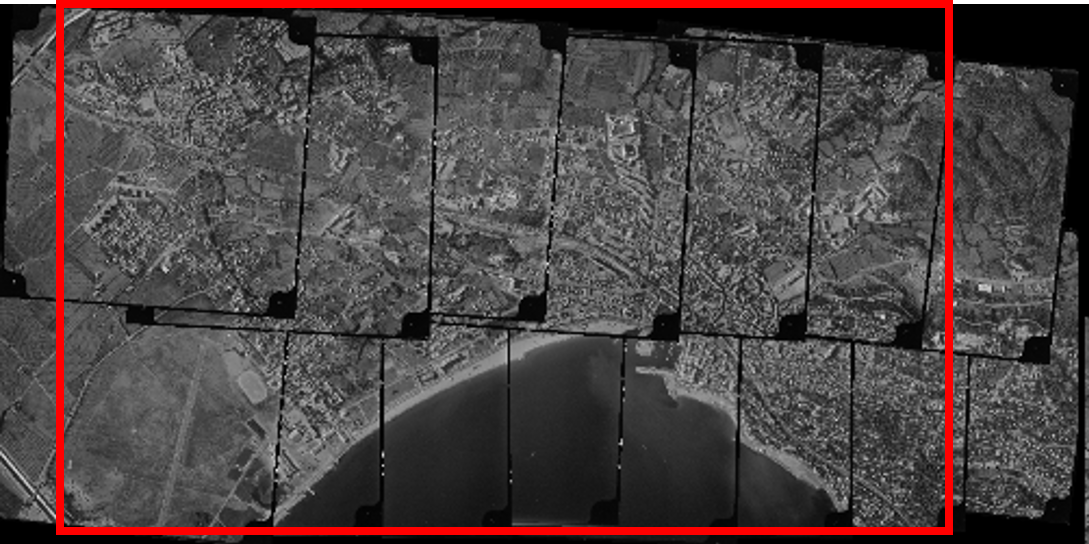
\includegraphics[width=7.6cm]{images/Chapitre3/Frejus1966.png}
%            \end{minipage}%
%        }
%        \subfigure[Fr{\'e}jus 1970 (19 images)]{
%    \begin{minipage}[t]{0.5\linewidth}
%        \centering
%        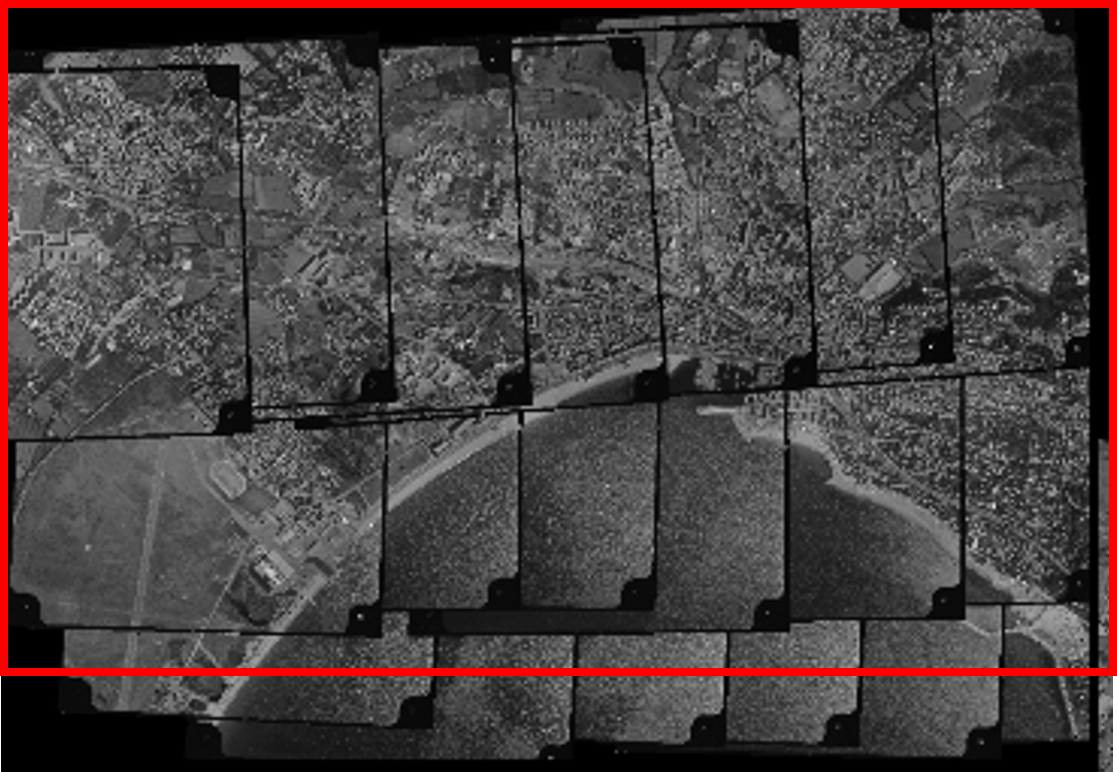
\includegraphics[width=6.1cm]{images/Chapitre3/Frejus1970.png}
%    \end{minipage}%
%}
%\subfigure[Fr{\'e}jus 2014 (36 images)]{
%    \begin{minipage}[t]{0.46\linewidth}
%        \centering
%        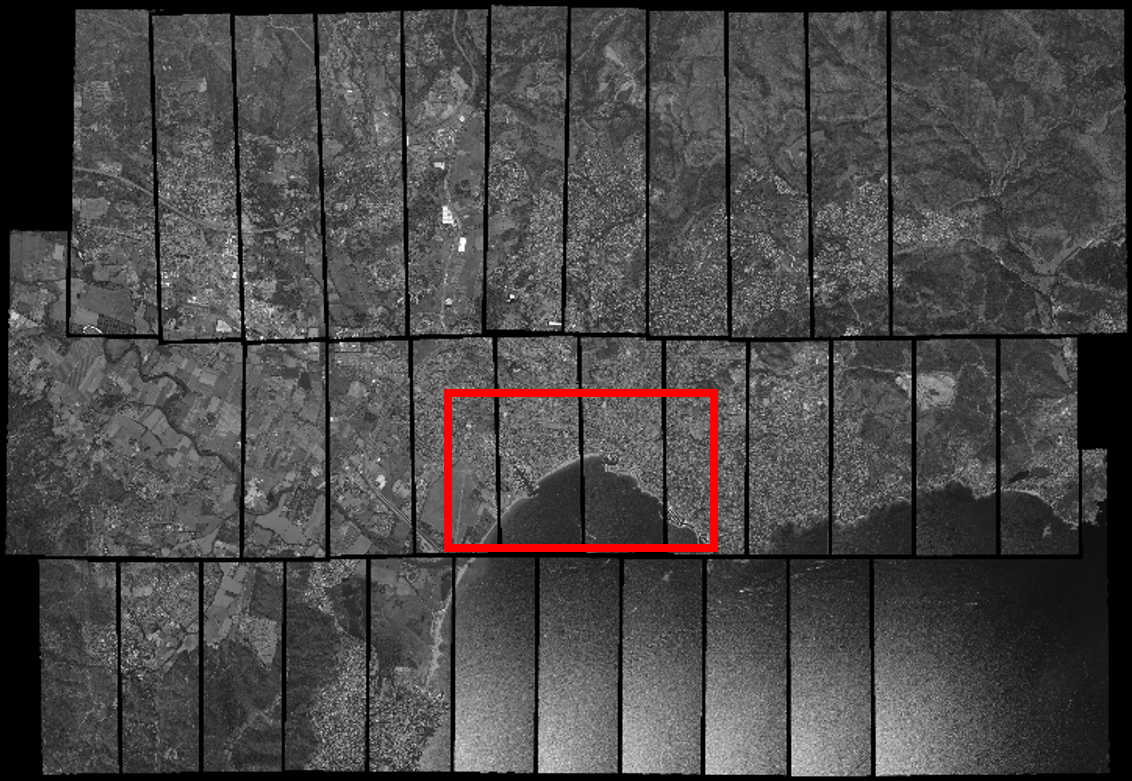
\includegraphics[width=6.25cm]{images/Chapitre3/Frejus2014.png}
%    \end{minipage}%
%}
%        \caption{Images demonstration of different aerial epochs in Fr{\'e}jus, image number of each epoch is displayed in the parenthesis of each sub headline. The overlapping zone between all the epochs is indicated by the red rectangles. Epoch 2014 is chosen as the reference epoch $E_r$ and the other epochs (i.e., epoch 1954, 1966 and 1970) are free epochs $E_f$ that should be co-registered to the frame of $E_r$. Graphic scale is demonstrated on $E_r$ in (d).}
%        \label{FrejusData}
%    \end{center}
%\end{figure*} 
%
%
%\begin{figure*}[htbp]
%    \begin{center}
%        \subfigure[Pezenas 1971 (57 images)]{
%            \begin{minipage}[t]{0.48\linewidth}
%                \centering
%                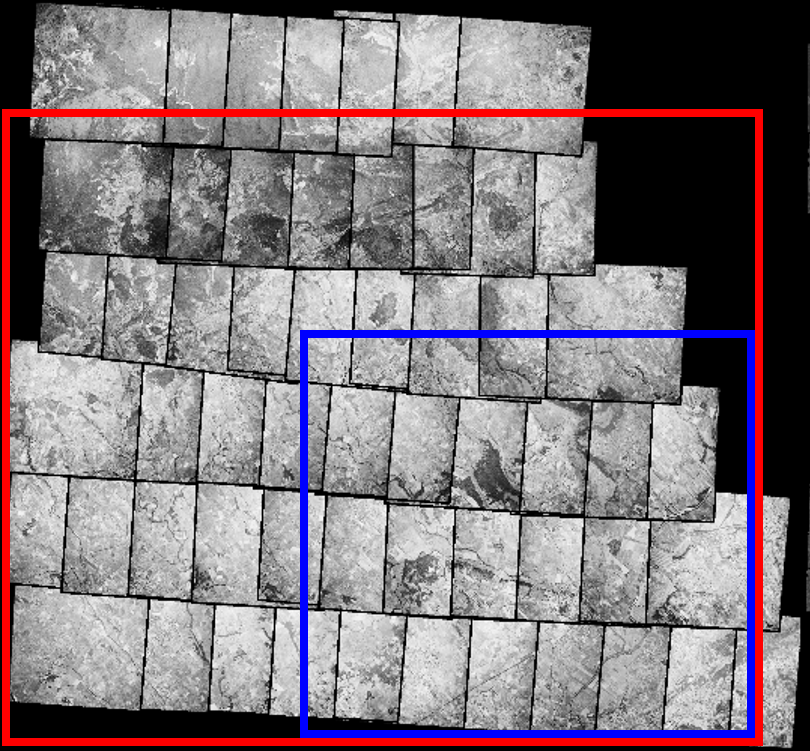
\includegraphics[width=6.45cm]{images/Chapitre3/Pezenas1971.png}
%            \end{minipage}%
%        }
%        \subfigure[Pezenas 1981 (27 images)]{
%            \begin{minipage}[t]{0.48\linewidth}
%                \centering
%                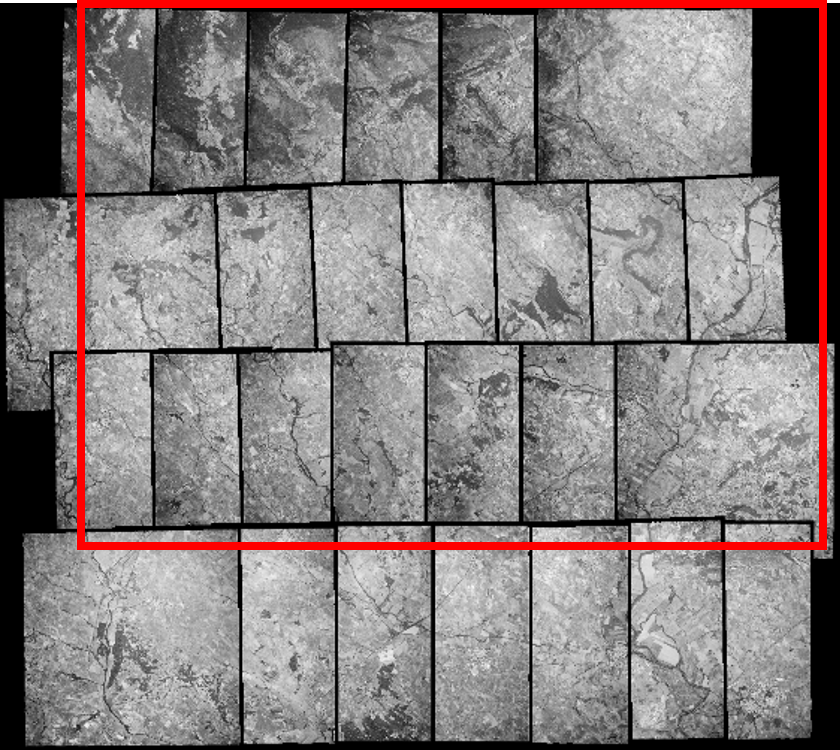
\includegraphics[width=6.68cm]{images/Chapitre3/Pezenas1981.png}
%            \end{minipage}%
%        }
%            \subfigure[Pezenas 2014 (2 satellite images)]{
%    	\begin{minipage}[t]{0.48\linewidth}
%    		\centering
%    		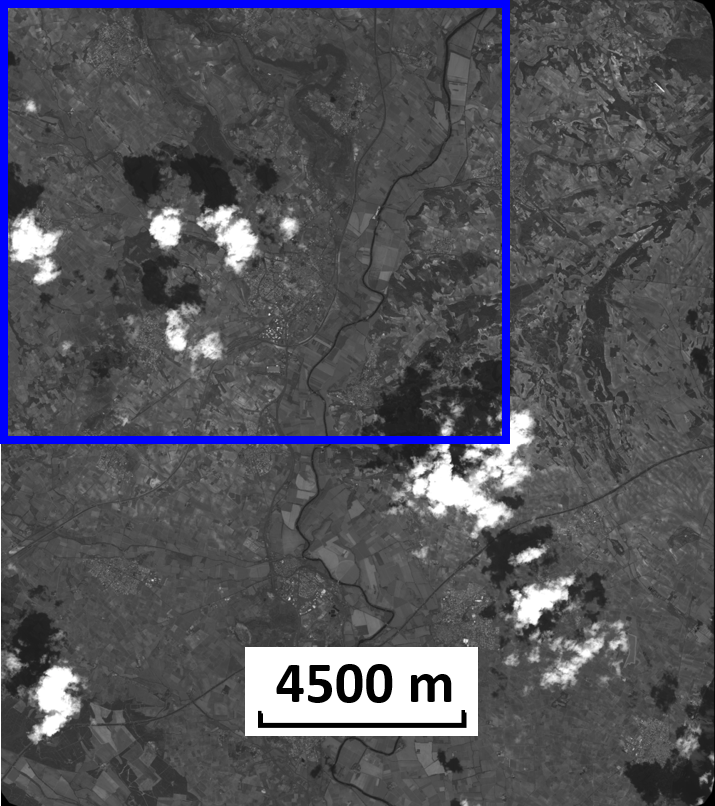
\includegraphics[width=6.6cm]{images/Chapitre3/Pezenas2014.png}
%    	\end{minipage}%
%    }
%        \subfigure[Pezenas 2015 (382 images)]{
%            \begin{minipage}[t]{0.48\linewidth}
%                \centering
%                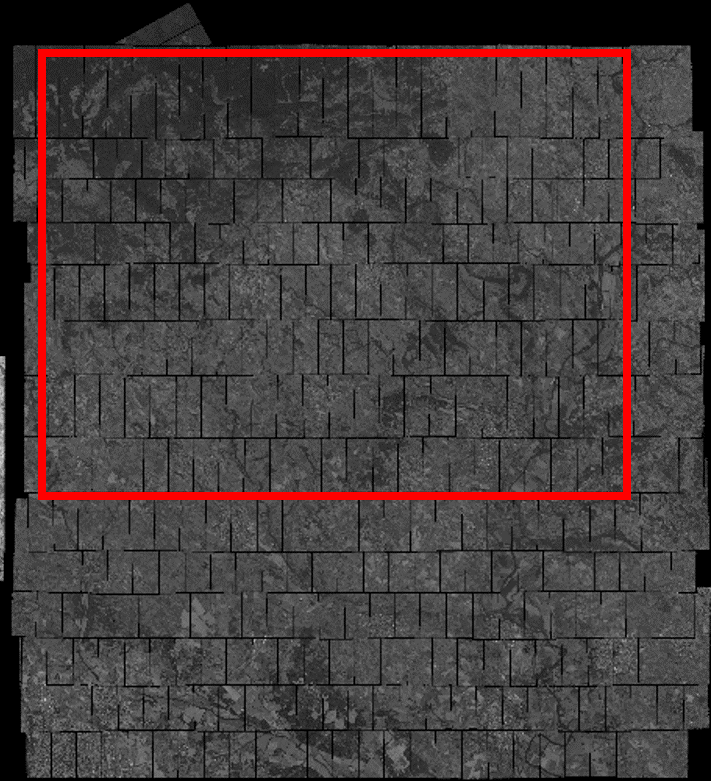
\includegraphics[width=6.78cm]{images/Chapitre3/Pezenas2015.png}
%            \end{minipage}%
%        }
%        \caption{Images demonstration of different aerial epochs as well as satellite epoch in Pezenas, image number of each epoch is displayed in the parenthesis of each sub headline. There are 2 historical aerial epochs (1971 and 1981) and 2 \ac{GT} epochs (2014 the satellite epoch and 2015 the aerial epoch) in this dataset. The overlapping zone between the historical epochs and the 2014 satellite epoch is indicated by the blue rectangles, while that between historical epochs and the 2015 aerial epoch is in red rectangles. Epoch 2014 and 2015 are chosen as the reference epoch $E_r$ and the other epochs (i.e., epoch 1971 and 1981) are free epochs $E_f$ that should be co-registered to the frame of $E_r$. Graphic scales are demonstrated on $E_r$ in (c) and (d).}
%        \label{PezenasData}
%    \end{center}
%\end{figure*} 
%
%
%\begin{figure*}[htbp]
%    \begin{center}
%        \subfigure[Kobe 1991 (15 images)]{
%            \begin{minipage}[t]{1\linewidth}
%                \centering
%                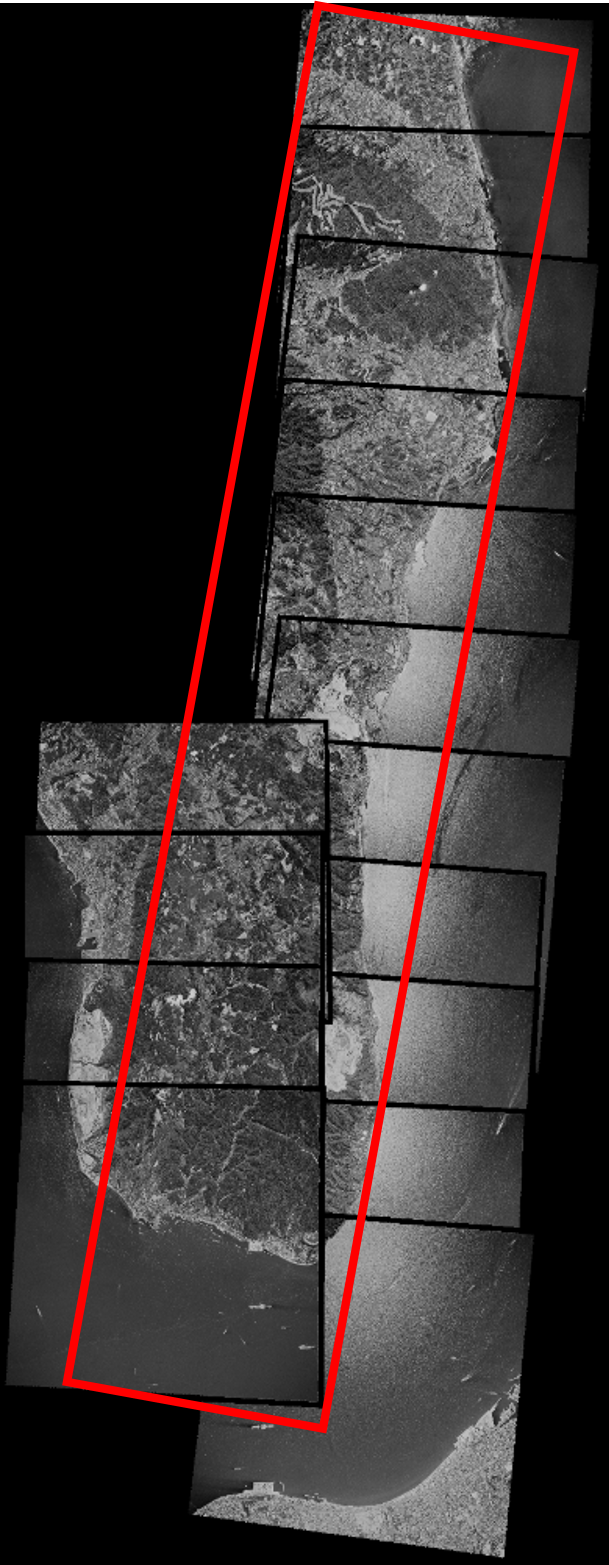
\includegraphics[height=13cm,angle=90]{images/Chapitre3/Kobe1991.png}
%            \end{minipage}%
%        }
%        \subfigure[Kobe 1995 (83 images)]{
%            \begin{minipage}[t]{1\linewidth}
%                \centering
%                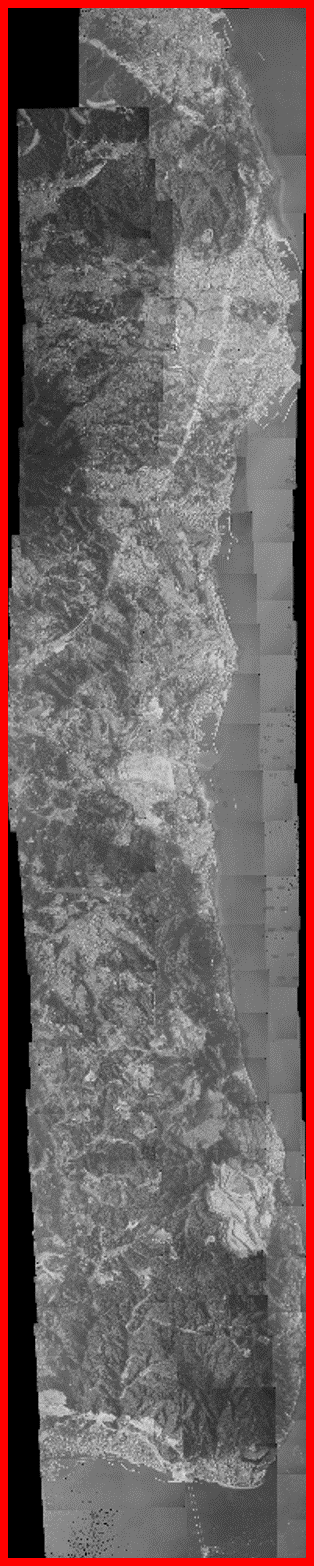
\includegraphics[height=13cm,angle=90]{images/Chapitre3/Kobe1995.png}
%            \end{minipage}%
%        }
%        \caption{Images demonstration of different aerial epochs in Kobe, image number of each epoch is displayed in the parenthesis of each sub headline. The overlapping zone between all the epochs is indicated by the red rectangles. Epoch 1995 is chosen as the reference epoch $E_r$ and the other epoch (i.e., epoch 1991) is free epoch $E_f$ that should be co-registered to the frame of $E_r$. Graphic scale is demonstrated on $E_r$ in (b).}
%        \label{KobeData}
%    \end{center}
%\end{figure*} 
%
%
%\begin{figure*}[htbp]
%	\begin{center}
%		\subfigure[Subregion of Fr{\'e}jus 1954]{
%			\begin{minipage}[t]{1\linewidth}
%				\centering
%				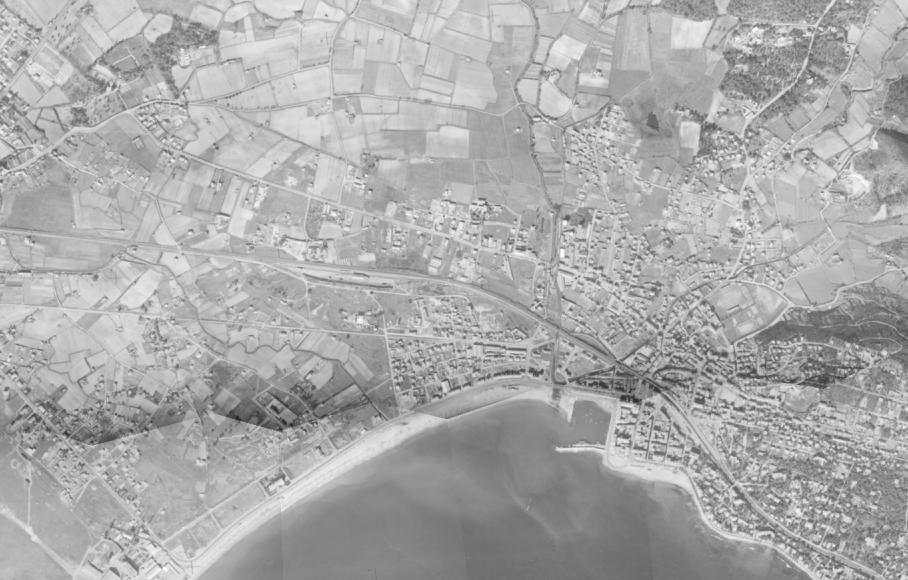
\includegraphics[width=13cm]{images/Chapitre3/Frejus1954Sub.png}
%			\end{minipage}%
%		}
%		\subfigure[Subregion of Fr{\'e}jus 2014]{
%			\begin{minipage}[t]{1\linewidth}
%				\centering
%				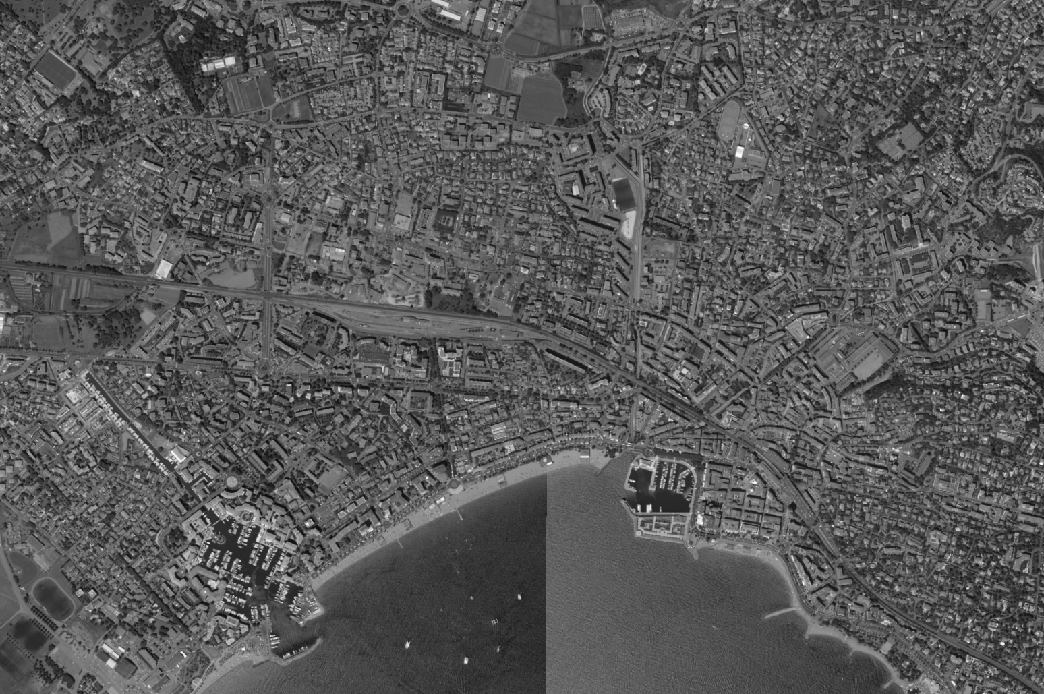
\includegraphics[width=13cm]{images/Chapitre3/Frejus2014Sub.png}
%			\end{minipage}%
%		}
%		\caption{Evolution of a subregion in Fr{\'e}jus.}
%		\label{FrejusEvolution}
%	\end{center}
%\end{figure*} 
%####################################End Dataset

\subsection{Implementation details}
\label{Implementationdetails}
%To improve efficiency, all input images are downsampled by a factor of 3 beforehand. To calculate the DSMs and orthophotos, we further downsample the images by a factor of 4, which amounts to a total downsampling factor of 12 with respect to the input images. For example, the images in Fr{\'e}jus 1970 are downsampled from [8766, 8763] to [730, 730]. As the goal of rough co-registration is to get robust rather than precise matches, a low resolution DSM/orthophoto is good enough and keeps the computational cost low. \\
To improve efficiency, all input images are downsampled by a factor of 3 beforehand, except for dataset Alberona as it consists of very few images. To calculate the \ac{DSM}s and orthophotos, we further downsample the images by a factor of 8, which amounts to a total downsampling factor of 24 with respect to the input images (total downsampling factor of 8 for Alberona). For example, the images in Fr{\'e}jus 1970 are downsampled from [8766, 8763] to [365, 365] for calculating \ac{DSM}s and orthophotos. As the goal of rough co-registration is to get robust rather than precise matches, a low resolution \ac{DSM}/orthophoto is good enough and keeps the computational cost low. \\
However, the downsampling factor of Fr{\'e}jus 2014 is set to be 12 instead of 24, as Fr{\'e}jus is mainly covered with buildings and the GSD of Fr{\'e}jus 2014 is too limited to tell details from \ac{DSM} with low resolution.\\%generated on images downsampled with factor 24.\\
%For each dataset, one epoch (generally the most recent epoch) would be chosen as the reference epoch, the remaining epochs would be treated as free epochs. The rough co-registration is applied on each free epoch and the reference epoch to obtain the co-registered image orientations in the frame of the reference epoch.
\zll{For each dataset, one epoch (generally the most recent epoch) is chosen as the reference epoch $E_r$, the others would be treated as free epoch $E_f$. The rough co-registration is applied between each free epoch $E_f$ and the reference epoch $E_r$. As a result, all free epochs $E_f$ would be moved to the frame of epoch $E_r$.\\ }
\zll{For the procedure of RANSAC to build (1) 3D Helmert transformation, we empirically set the number of iteration to 2000, and $T_r$ to 50m; (2) 2D similarity transformation, we set the number of iteration to 1000, and $T_r$ to 15 pixels. For the \textit{one-to-many tiling scheme}, the tile size $SZ_{one-to-many}$ is set to be 1280$\times$960 pixels to balance performance and efficiency. }
%in our experiment
%For variants $SuperGlue_{ImgPairs}$, $SuperGlue_{Ortho}$ and $SuperGlue_{DSM}$, 
All the image/tile pairs entering SuperGlue are downsampled to 640$\times$480 pixels, as it is the default parameter provided by the author and guarantees the best performance. 
%For the tiling scheme in $SuperGlue_{Ortho}$ and $SuperGlue_{DSM}$, orthophotos/DSMs are split to tiles of the size 1280$\times$960 pixels.


\subsection{Comparison between $SIFT_{Adapted}$ and $SIFT_{Default}$}
\label{Compare2SIFTs}
In this section, two different sets of SIFT parameters are compared, which are referred to as $SIFT_{Default}$ and $SIFT_{Adapted}$:\\
\begin{enumerate}
	\item \textbf{$SIFT_{Default}$}: Extract SIFT keypoints on the original images, followed by mutual nearest neighbor matching combined with ratio test.% and FIGNN (REF).
	%\item \textbf{$SIFT_{Adapted}$}: Downsample the input images with a factor of 3 and extract SIFT keypoints, match them by mutual nearest neighbor without ratio test and FIGNN, followed by applying RANSAC based on 2D similarity transformation model to remove outliers.
	\item \textbf{$SIFT_{Adapted}$}: Downsample the input images with a factor of 3 and extract SIFT keypoints, match them by mutual nearest neighbor without ratio test, followed by applying RANSAC based on 2D similarity transformation model to remove outliers.
\end{enumerate}

%Comparison between $SIFT_{Default}$ and $SIFT_{Adapted}$ on pipelines ${ImgPairs}$, ${Ortho}$ and ${DSM}$ are demonstrated individually in the following sections.
%Experiments comparing $SIFT_{Default}$ and $SIFT_{Adapted}$ on variants ${ImgPairs}$, ${Ortho}$ and ${DSM}$ are displayed in section ~\ref{Compare2SIFTs}, %Appendix ~\ref{chap:appendix1}, 
%in which $SIFT_{Adapted}$ recovered enough good matches while $SIFT_{Default}$ failed. It is reasonable as inter-epoch images often look very different, $SIFT_{Default}$ generally recover very few matches. By downsamping the images, we are able to focus on the global outline of the scene for improving robustness. 
%By relaxing the matching restriction of ratio test, right matches would be preserved while wrong matches would be removed in the subsequent RANSAC.\\

%\subsubsection{Comparison on matching image pair}
\paragraph{Results on matching image pairs.}
For pipeline ${ImgPairs}$, we choose a pair of images from dataset Pezenas consists of images taken at 1971 and 2015 individually. The results are displayed in Figure \ref{SIFTComp_ImgPair}. As can be seen, $SIFT_{Adapted}$ recovers 101 good matches out of 2592 total matches, however, $SIFT_{Default}$ finds only 3 matches in total, even though 2 of them are correct matches, it is impossible for the RANSAC procedure to screen the correct ones.\\
\begin{figure*}[htbp]
	\begin{center}
		\subfigure[Image pair]{
			\begin{minipage}[t]{0.48\linewidth}
				\centering
				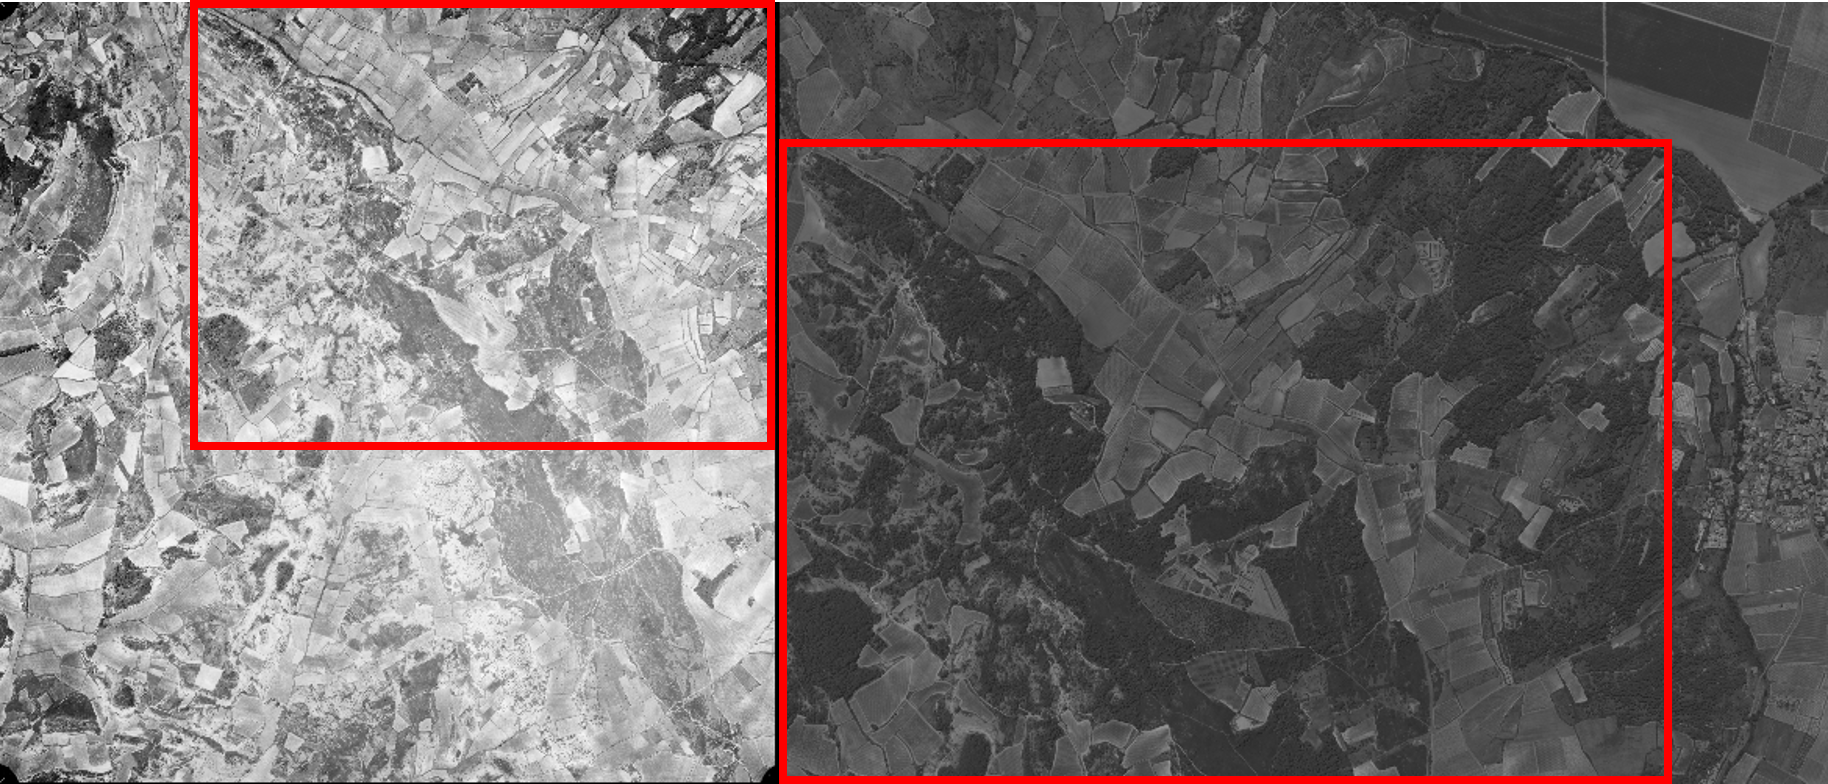
\includegraphics[width=7.5cm]{images/appendix/OIS-Reech_IGNF_PVA_1-0__1971-06-21__C2844-0141_1971_FR2117_1124_15FD3425x00034_02911.png}
			\end{minipage}%
		}
		\subfigure[Number of recovered matches]{
			\begin{minipage}[t]{0.48\linewidth}
				\centering
				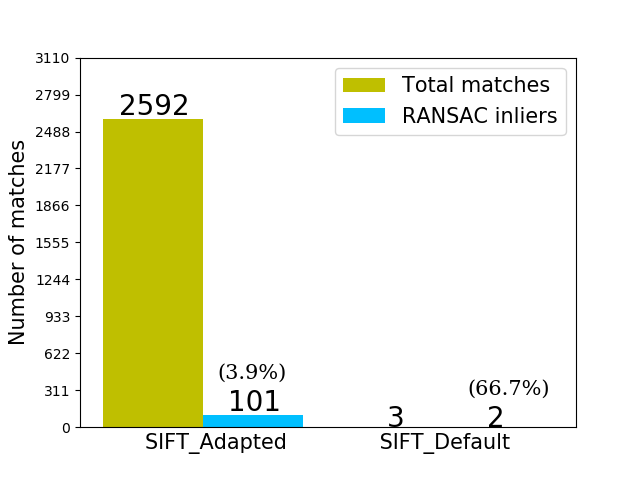
\includegraphics[width=4.8cm]{images/appendix/PlotCurves-SIFTComp_OIS-Reech_IGNF_PVA_1-0__1971-06-21__C2844-0141_1971_FR2117_1124_15FD3425x00034_02911.png}
			\end{minipage}%
		}
		\subfigure[$SIFT_{Adapted}^{RANSAC Inliers}$]{
			\begin{minipage}[t]{0.48\linewidth}
				\centering
				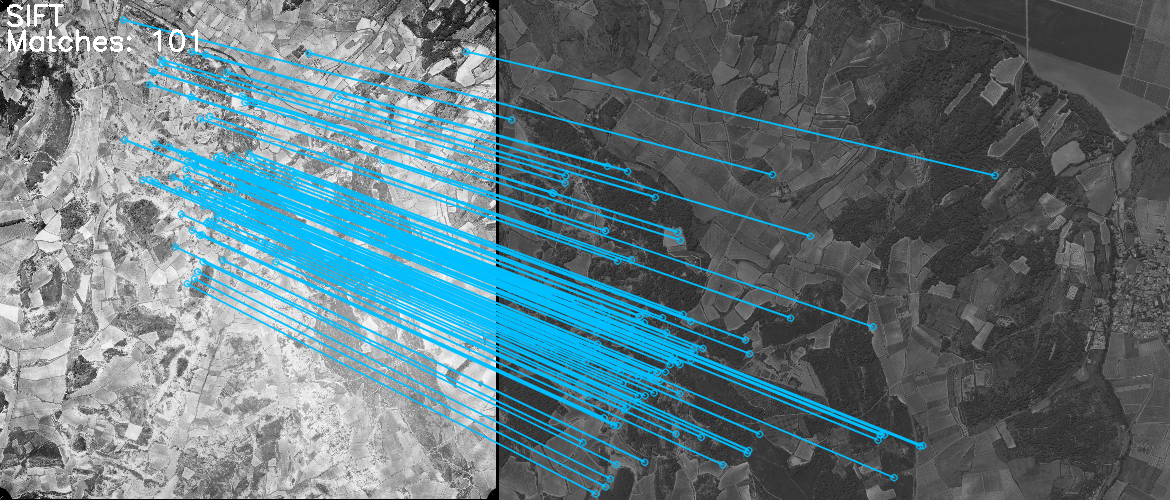
\includegraphics[width=6cm]{images/appendix/Homol-SIFT2Step_Test-Rough-2DRANSAC_OIS-Reech_IGNF_PVA_1-0__1971-06-21__C2844-0141_1971_FR2117_1124_15FD3425x00034_02911.png}
			\end{minipage}%
		}
		\subfigure[$SIFT_{Default}^{TotalMatches}$]{
			\begin{minipage}[t]{0.48\linewidth}
				\centering
				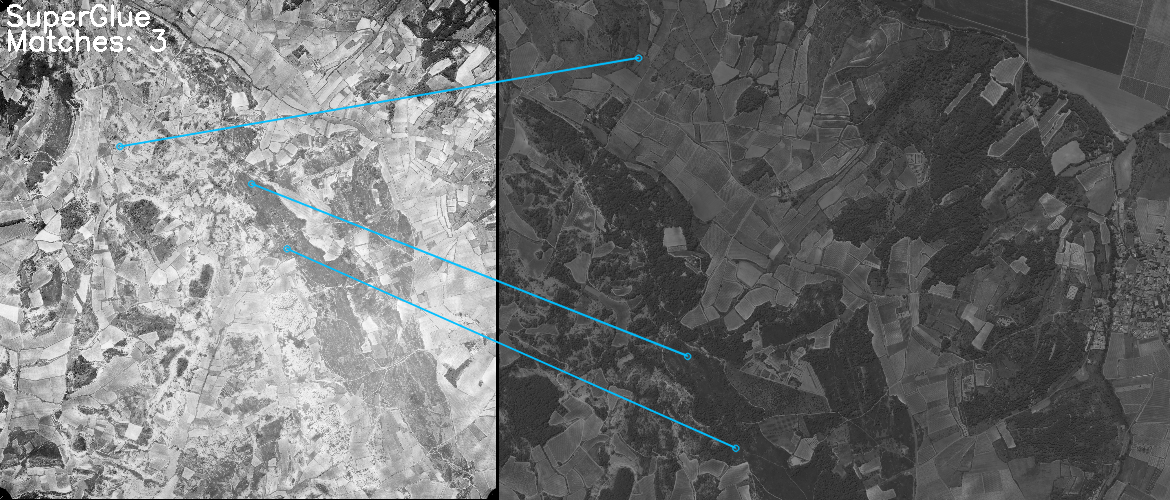
\includegraphics[width=6cm]{images/appendix/Homol-txt_OIS-Reech_IGNF_PVA_1-0__1971-06-21__C2844-0141_1971_FR2117_1124_15FD3425x00034_02911.png}
			\end{minipage}%
		}
		\caption{Comparison between $SIFT_{Adapted}$ and $SIFT_{Default}$ on a pair of images from Pezenas 1971 and Pezenas 2015 individually. (a) Image pair to be matched, with red rectangles indicating the overlapping zone. (b) Numbers of total matches and RANSAC inliers of $SIFT_{Adapted}$ and $SIFT_{Default}$. (c) Visualization of RANSAC inliers based on $SIFT_{Adapted}$. (d)Visualization of total matches based on $SIFT_{Default}$.}
		\label{SIFTComp_ImgPair}
	\end{center}
\end{figure*} 

%\subsubsection{Comparison on matching orthophotos}
\paragraph{Results on matching orthophotos.}
For pipeline ${Ortho}$, we choose orthophotos from Pezenas 1981 and 2015 individually. The results are displayed in Figure \ref{SIFTComp_Ortho}. As can be seen, $SIFT_{Adapted}$ recovers 44 good matches out of 855 total matches, while $SIFT_{Default}$ finds 8 total matches which are all wrong.\\
\begin{figure*}[htbp]
	\begin{center}
		\subfigure[Orthophotos]{
			\begin{minipage}[t]{0.48\linewidth}
				\centering
				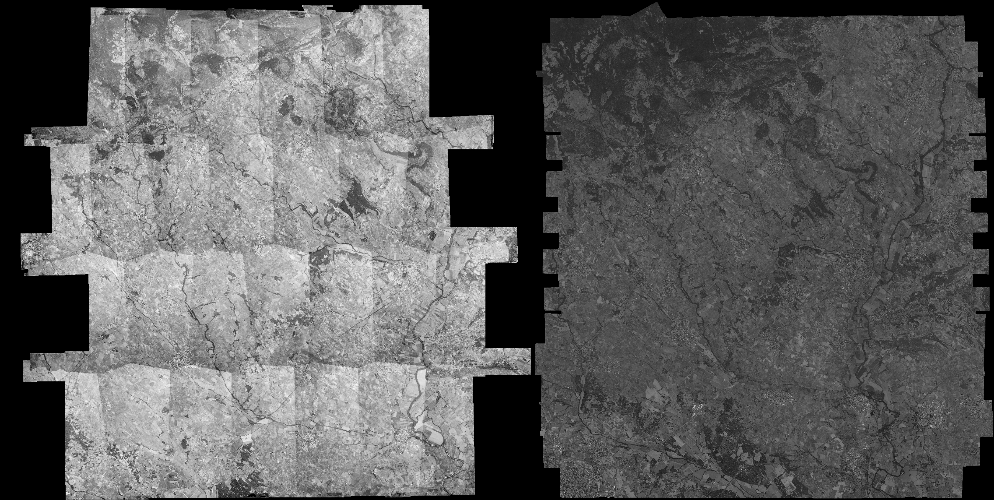
\includegraphics[width=7.5cm]{images/Chapitre3/Ortho-MEC-Malt_Tapas_1981_Ortho-MEC-Malt_2015.png}
			\end{minipage}%
		}
		\subfigure[Number of recovered matches]{
			\begin{minipage}[t]{0.48\linewidth}
				\centering
				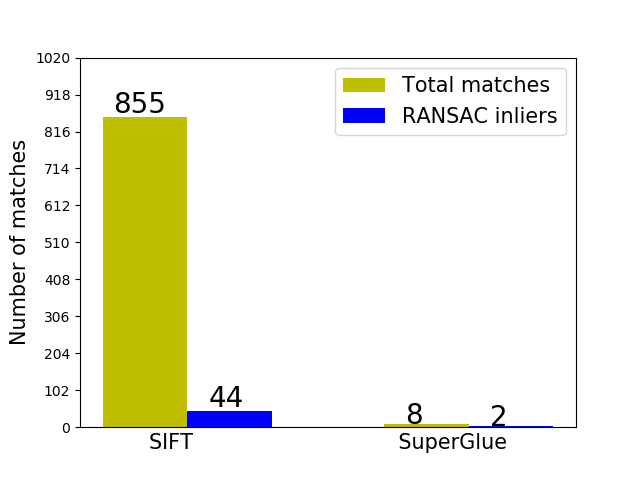
\includegraphics[width=4.8cm]{images/appendix/PlotCurves-SIFTComp_Ortho-MEC-Malt_Tapas_1981_Ortho-MEC-Malt_2015.png}
			\end{minipage}%
		}
		\subfigure[$SIFT_{Adapted}^{RANSAC Inliers}$]{
			\begin{minipage}[t]{0.48\linewidth}
				\centering
				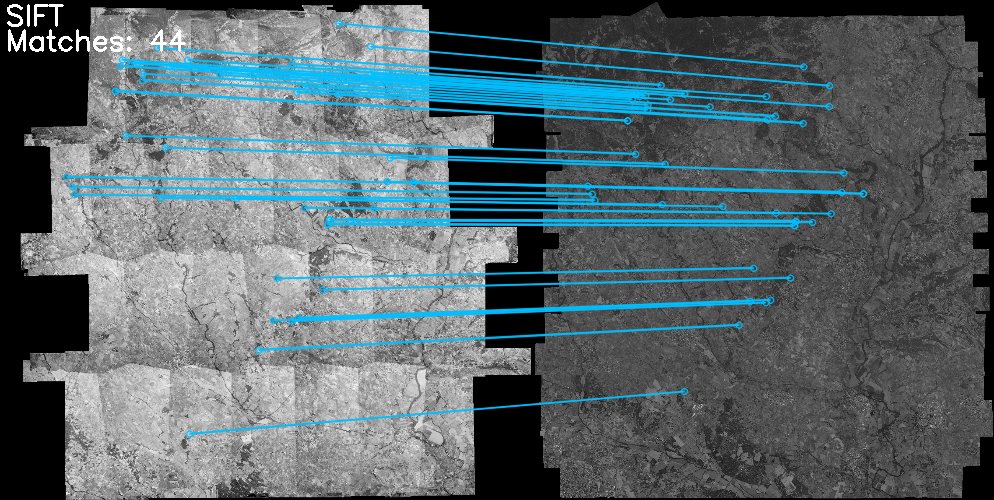
\includegraphics[width=6cm]{images/appendix/Homol-SIFT2Step-Rough-2DRANSAC_Ortho-MEC-Malt_Tapas_1981_Ortho-MEC-Malt_2015.png}
			\end{minipage}%
		}
		\subfigure[$SIFT_{Default}^{TotalMatches}$]{
			\begin{minipage}[t]{0.48\linewidth}
				\centering
				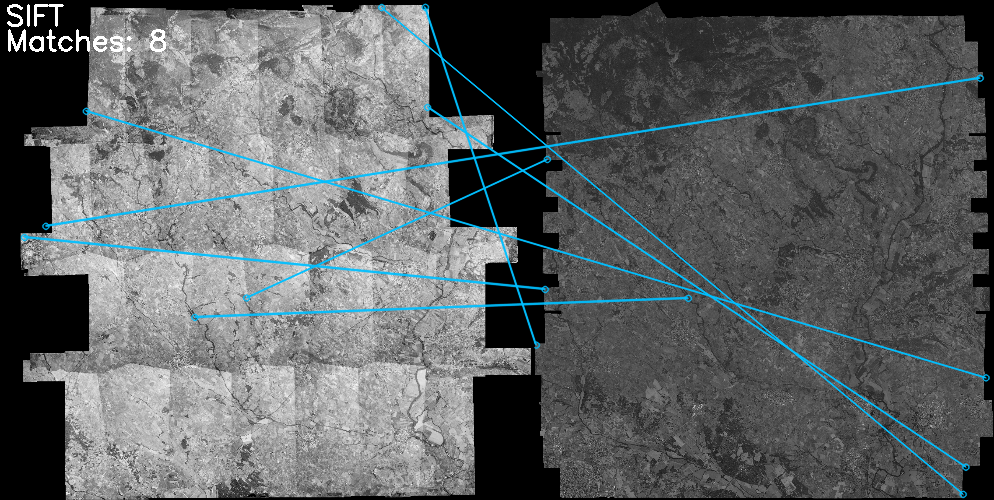
\includegraphics[width=6cm]{images/appendix/Homol-SIFT_Ortho-MEC-Malt_Tapas_1981_Ortho-MEC-Malt_2015.png}
			\end{minipage}%
		}
		\caption{Comparison between $SIFT_{Adapted}$ and $SIFT_{Default}$ on orthophotos from Pezenas 1981 and Pezenas 2015 individually. (a) Orthophotos to be matched, with red rectangles indicating the overlapping zone. (b) Numbers of total matches and RANSAC inliers of $SIFT_{Adapted}$ and $SIFT_{Default}$. (c) Visualization of RANSAC inliers based on $SIFT_{Adapted}$. (d)Visualization of total matches based on $SIFT_{Default}$.}
		\label{SIFTComp_Ortho}
	\end{center}
\end{figure*} 

%\subsubsection{Comparison on matching DSMs}
\paragraph{Results on matching \ac{DSM}s.}
For pipeline ${DSM}$, we choose \ac{DSM}s from Fr{\'e}jus 1954 and 2014 individually. The results are displayed in Figure \ref{SIFTComp_DSM}. As drastic scene changes are displayed in dataset Fr{\'e}jus, $SIFT_{Default}$ fails to find any matches. $SIFT_{Adapted}$, however, recovers 11 good matches, even though the inlier ratio is dangerously low (i.e., 0.5\%).\\
\begin{figure*}[htbp]
	\begin{center}
		\subfigure[\ac{DSM}s]{
			\begin{minipage}[t]{0.58\linewidth}
				\centering
				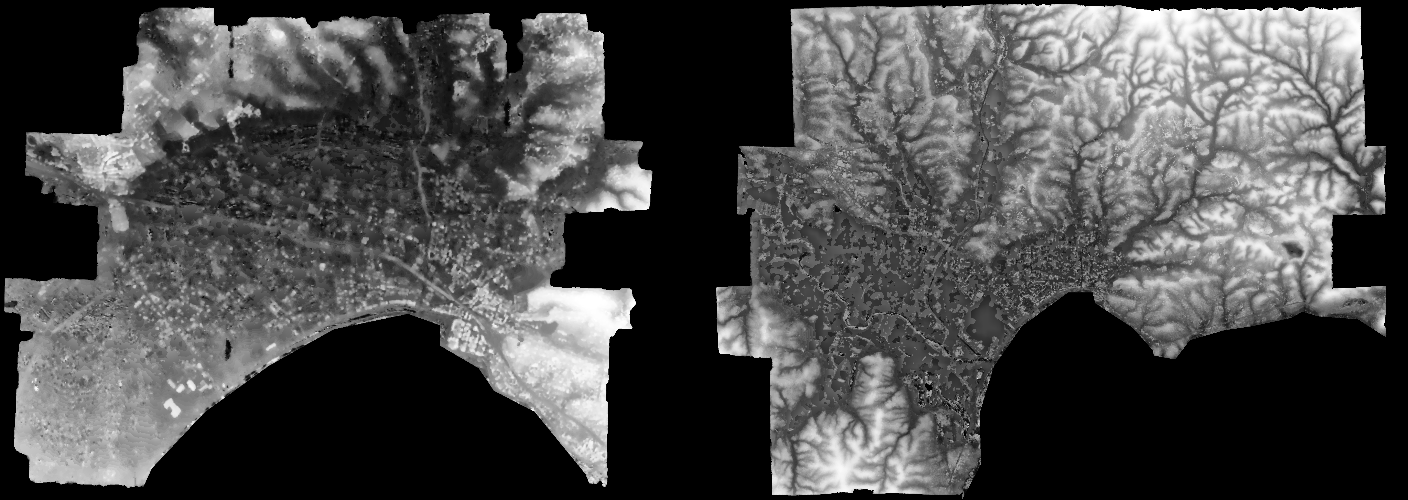
\includegraphics[width=8.2cm]{images/Chapitre3/MEC-Malt_Tapas_1954_MEC-Malt_2014.png}
			\end{minipage}%
		}
		\subfigure[Number of recovered matches]{
			\begin{minipage}[t]{0.38\linewidth}
				\centering
				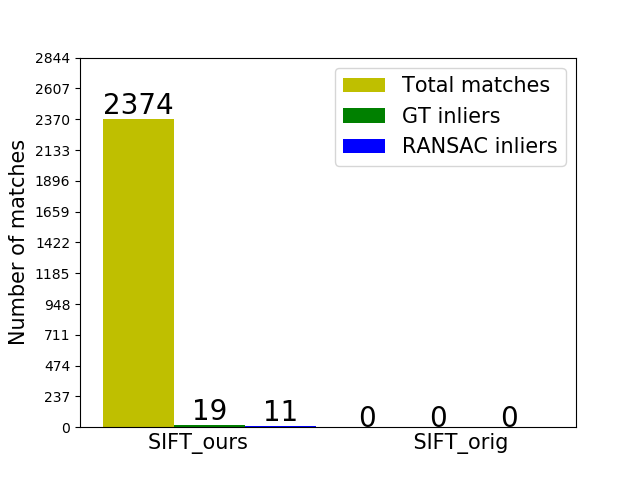
\includegraphics[width=4.8cm]{images/appendix/PlotCurves-SIFTComp_MEC-Malt_Tapas_1954_MEC-Malt_2014.png}
			\end{minipage}%
		}
		\subfigure[$SIFT_{Adapted}^{RANSAC Inliers}$]{
			\begin{minipage}[t]{0.48\linewidth}
				\centering
				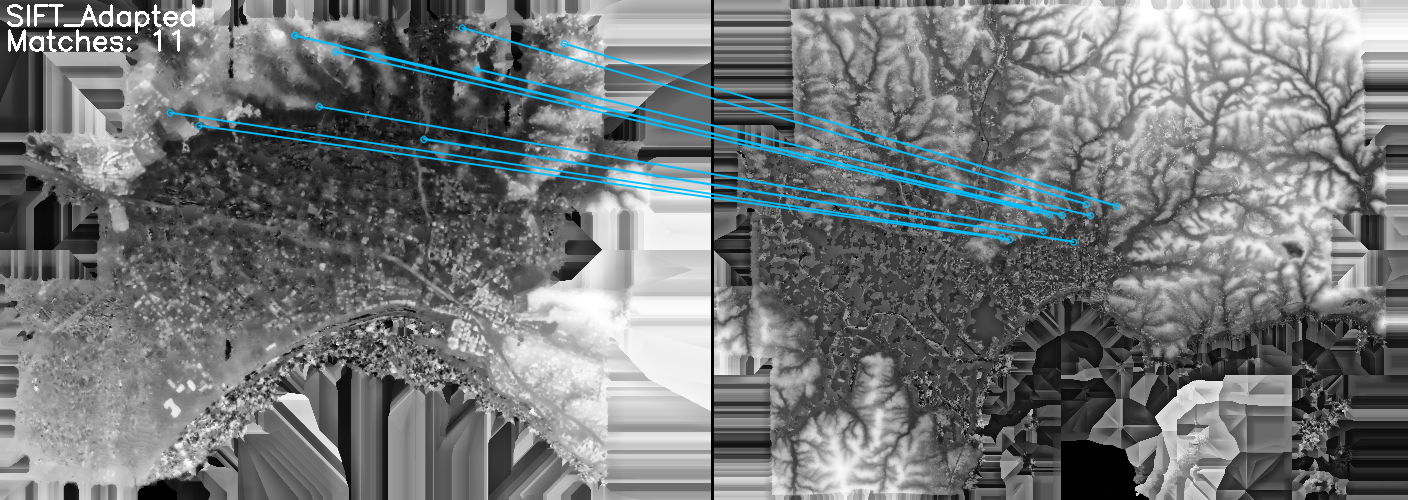
\includegraphics[width=6.8cm]{images/appendix/Homol-SIFT2Step-Rough-2DRANSAC_MEC-Malt_Tapas_1954_MEC-Malt_2014.png}
			\end{minipage}%
		}
		\subfigure[$SIFT_{Default}^{TotalMatches}$]{
			\begin{minipage}[t]{0.48\linewidth}
				\centering
				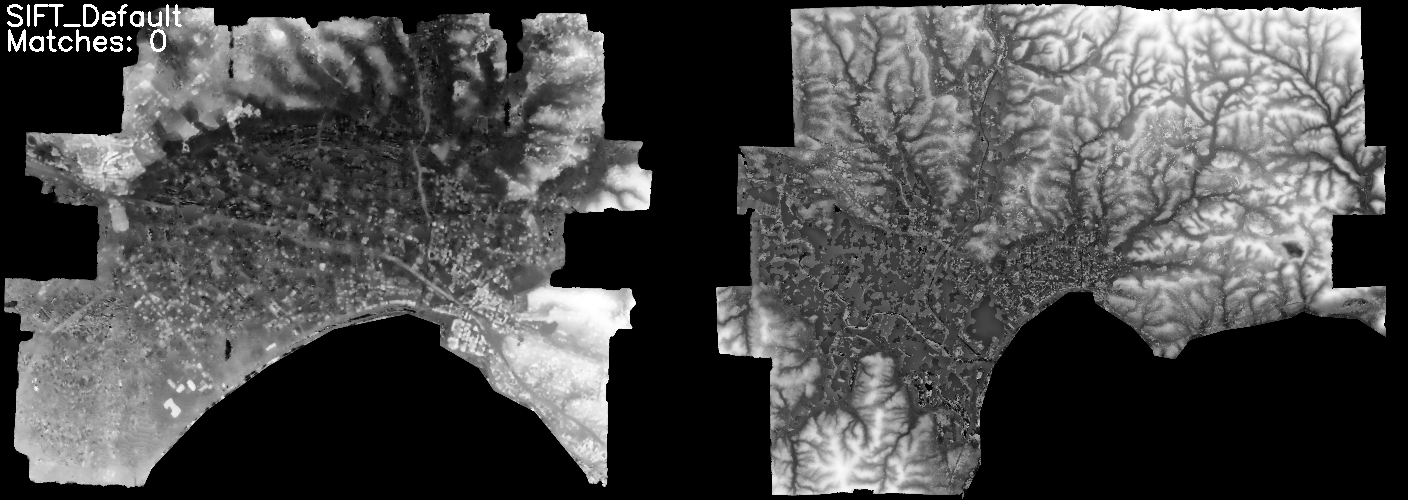
\includegraphics[width=6.8cm]{images/appendix/Homol-txt_MEC-Malt_Tapas_1954_MEC-Malt_2014.png}
			\end{minipage}%
		}
		\caption{Comparison between $SIFT_{Adapted}$ and $SIFT_{Default}$ on \ac{DSM}s from Fr{\'e}jus 1954 and Fr{\'e}jus 2014 individually. (a) \ac{DSM}s to be matched, with red rectangles indicating the overlapping zone. (b) Numbers of total matches and RANSAC inliers of $SIFT_{Adapted}$ and $SIFT_{Default}$. (c) Visualization of RANSAC inliers based on $SIFT_{Adapted}$. (d)Visualization of total matches based on $SIFT_{Default}$.}
		\label{SIFTComp_DSM}
	\end{center}
\end{figure*} 

In general, $SIFT_{Adapted}$ recovers enough good matches in all the 3 variants ($SIFT_{ImgPairs}$, $SIFT_{Ortho}$ and $SIFT_{DSM}$), while $SIFT_{Default}$ fails. It is reasonable as inter-epoch images often look very different, $SIFT_{Default}$ generally recover very few matches. By downsampling the images, we are able to focus on the global outline of the scene to improve robustness. 
By relaxing the matching restriction of ratio test, right matches would be preserved while wrong matches would be removed in the subsequent RANSAC.\\


\subsection{Comparison between $SuperGlue_{tiling}$ and $SuperGlue_{orig}$}
\label{Compare2SpGs}
In order to explore whether the \textit{one-to-many tiling scheme} improves the performance of SuperGlue, 
we compare 2 sets of the results on matching multi-epoch orthophotos and \ac{DSM}s with $SuperGlue_{tiling}$ and $SuperGlue_{orig}$. The former and latter stands for SuperGlue combined with and without our \textit{one-to-many tiling scheme}. %As can be seen, $SuperGlue_{orig}$ failed while $SuperGlue_{tiling}$ recovered a large number of good matches.
%we compare the results of SuperGlue with and without the \textit{one-to-many tiling scheme} (i.e., $SuperGlue_{tiling}$ and $SuperGlue_{orig}$) on matching orthophotos and \ac{DSM}s. 
We chose the orthophotos and \ac{DSM}s from Fr{\'e}jus 1970 and 2014 individually for testing.\\
\zll{The sizes of the orthophotos and \ac{DSM}s are listed in Table \ref{ImgSize}. As mentioned in Section \ref{Implementationdetails}, the tile size $SZ_{one-to-many}$ is set to be 1280$\times$960 pixels, and the image/tile pairs in both $SuperGlue_{tiling}$ and $SuperGlue_{orig}$ are downsampled to 640$\times$480 pixels before entering SuperGlue. The comparison of downsampling ratio between $SuperGlue_{tiling}$ and $SuperGlue_{orig}$ for orthophotos and \ac{DSM}s from Fr{\'e}jus 1970 and 2014 is demonstrated in Table \ref{ImgDownRatio}.}
\begin{table}%[H]
	\centering
	\begin{tabular}{||l|c|c|c|c||}\hline
		 & \multicolumn{2}{c|}{orthophoto} & \multicolumn{2}{c||}{\ac{DSM}} \\\hline
		 & Width [pix] & Height [pix] & Width [pix] & Height [pix] \\\hline\hline
		E1970 & 899 & 618 & 3323 & 2394 \\\hline
		E2014 & 1124 & 773 & 4154 & 2992 \\\hline
	\end{tabular}
	\caption{Size of orthophotos and \ac{DSM}s from Fr{\'e}jus 1970 and 2014.}
	\label{ImgSize}
\end{table}
\begin{table}%[H]
	\centering
	\begin{tabular}{||l|c|c|c|c|c||}\hline
		& & \multicolumn{2}{c|}{orthophoto} & \multicolumn{2}{c||}{\ac{DSM}} \\\hline
		& & Width & Height & Width & Height \\\hline\hline
		\multirow{2}{*}{E1970} & $SuperGlue_{orig}$ & 1.4 & 1.3 & 1.8 & 1.6 \\
		 & $SuperGlue_{tiling}$ & 2 & 2 & 2 & 2 \\\hline
		\multirow{2}{*}{E2014} & $SuperGlue_{orig}$ & 5.2 & 5.0 & 6.5 & 6.2 \\
		 & $SuperGlue_{tiling}$ & 2 & 2 & 2 & 2 \\\hline
	\end{tabular}
	\caption{Comparison of downsampling ratio between $SuperGlue_{tiling}$ and $SuperGlue_{orig}$ for both orthophotos and \ac{DSM}s from Fr{\'e}jus 1970 and 2014.}
	\label{ImgDownRatio}
\end{table}

%\subsubsection{Comparison on matching orthophotos}
\paragraph{Results on matching orthophotos.}
Figure~\ref{MatchOrtho} displays the results of matching orthophotos with $SuperGlue_{tiling}$ and $SuperGlue_{orig}$. As can be seen, the former recovers 58 good matches with an inlier ratio reached 33\%, while the latter fails to find any correct matches.\\
\begin{figure*}[htbp]
	\begin{center}
		\subfigure[Orthophotos]{
			\begin{minipage}[t]{0.48\linewidth}
				\centering
				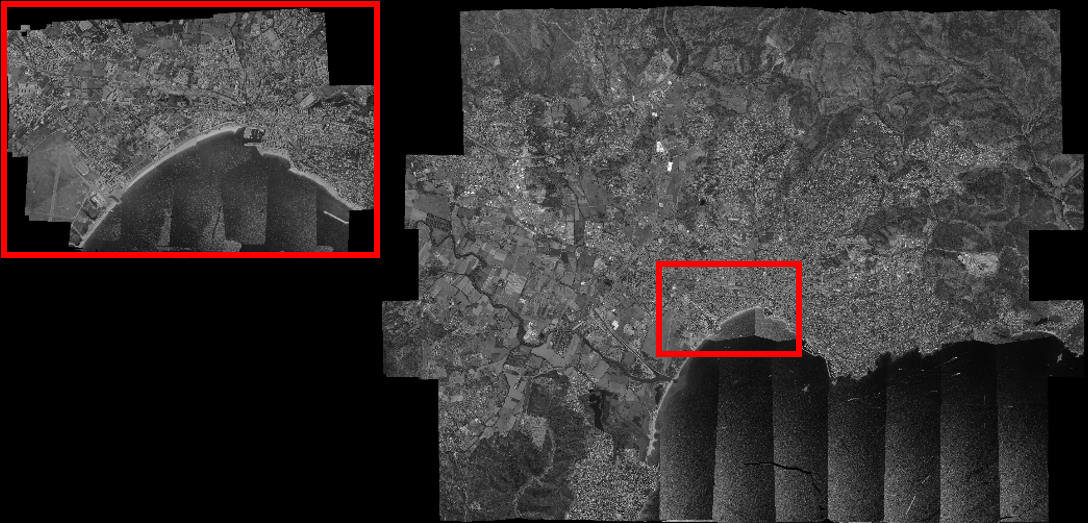
\includegraphics[width=7.5cm]{images/Chapitre3/Ortho-MEC-Malt_Tapas_1970_Ortho-MEC-Malt_2014.png}
			\end{minipage}%
		}
		\subfigure[Number of recovered matches]{
			\begin{minipage}[t]{0.48\linewidth}
				\centering
				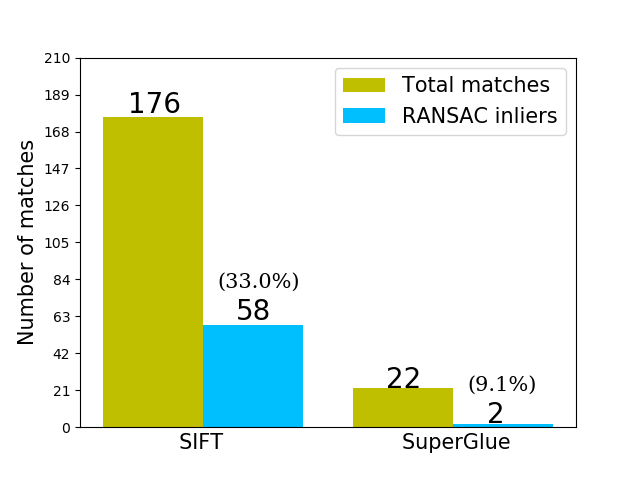
\includegraphics[width=4.8cm]{images/appendix2/PlotCurves_TileTest-Ortho-MEC-Malt_Tapas_1970_Ortho-MEC-Malt_2014.png}
			\end{minipage}%
		}
		\subfigure[$SuperGlue_{tiling}^{RANSAC Inliers}$]{
			\begin{minipage}[t]{0.48\linewidth}
				\centering
				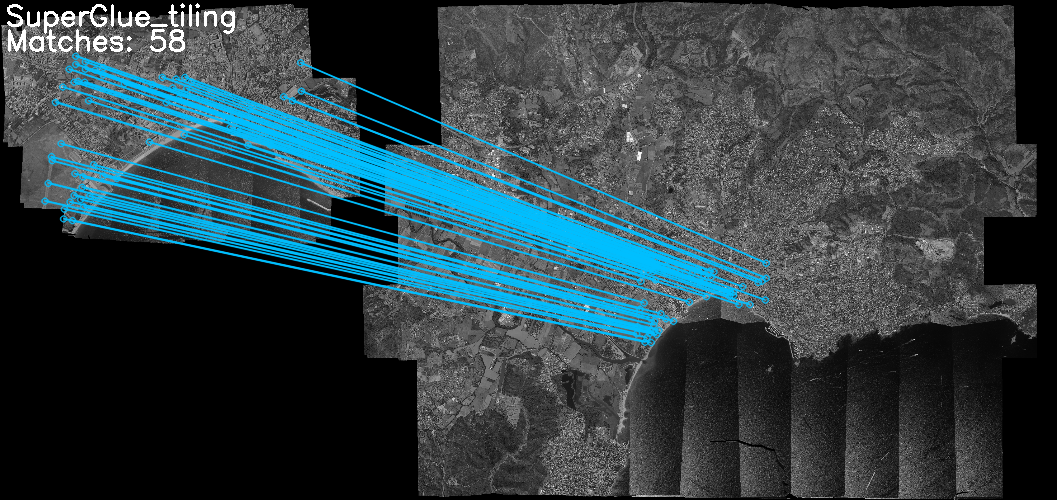
\includegraphics[width=6cm]{images/appendix2/Homol-SubPatch_R270-2DRANSAC_Ortho-MEC-Malt_Tapas_1970_Ortho-MEC-Malt_2014.png}
			\end{minipage}%
		}
		\subfigure[$SuperGlue_{orig}^{TotalMatches}$]{
			\begin{minipage}[t]{0.48\linewidth}
				\centering
				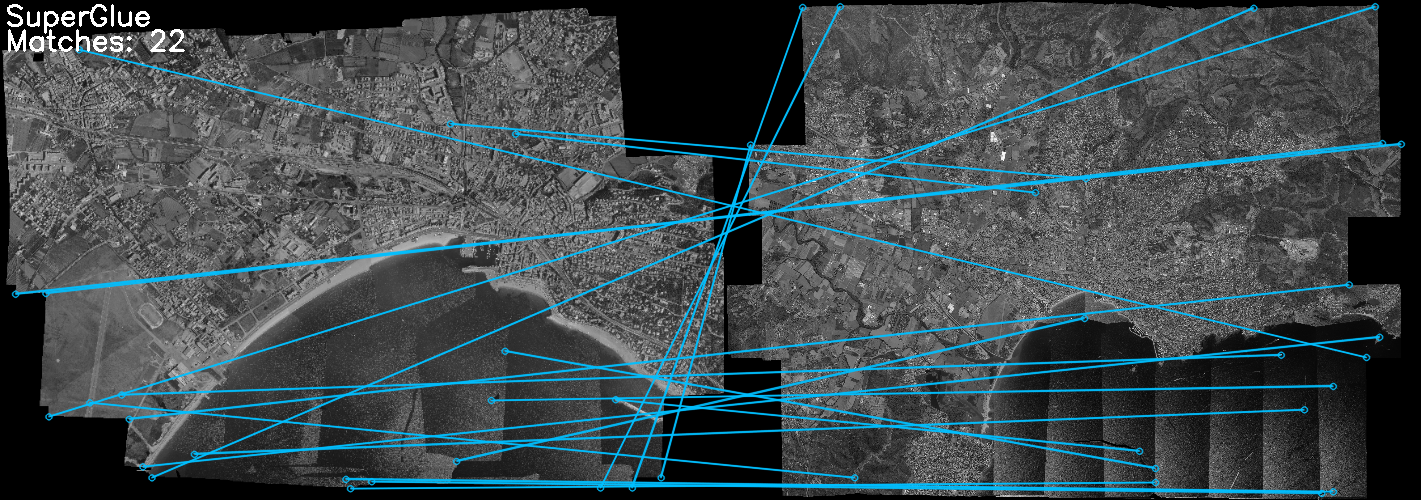
\includegraphics[width=6cm]{images/appendix2/Homol-SuperGlue_Ortho-MEC-Malt_Tapas_1970_Ortho-MEC-Malt_2014.png}
			\end{minipage}%
		}
		\caption{Comparison between $SuperGlue_{tiling}$ and $SuperGlue_{orig}$ on orthophotos from Fr{\'e}jus 1970 and 2014 individually. (a) Orthophotos to be matched, with red rectangles indicating the overlapping zone. (b) Numbers of total matches and RANSAC inliers of $SuperGlue_{tiling}$ and $SuperGlue_{orig}$. (c) Visualization of RANSAC inliers based on $SuperGlue_{tiling}$. (d)Visualization of total matches based on $SuperGlue_{orig}$.}
		\label{MatchOrtho}
	\end{center}
\end{figure*} 

%\subsubsection{Comparison on matching \ac{DSM}s}
\paragraph{Results on matching \ac{DSM}s.}
Figure~\ref{MatchDSM} displays the results of matching \ac{DSM}s with $SuperGlue_{tiling}$ and $SuperGlue_{orig}$. As can be seen, the former recovers 190 good matches with an inlier ratio reached 46.5\%, while the latter fails to find any correct matches.\\
\begin{figure*}[htbp]
	\begin{center}
		\subfigure[\ac{DSM}s]{
			\begin{minipage}[t]{0.48\linewidth}
				\centering
				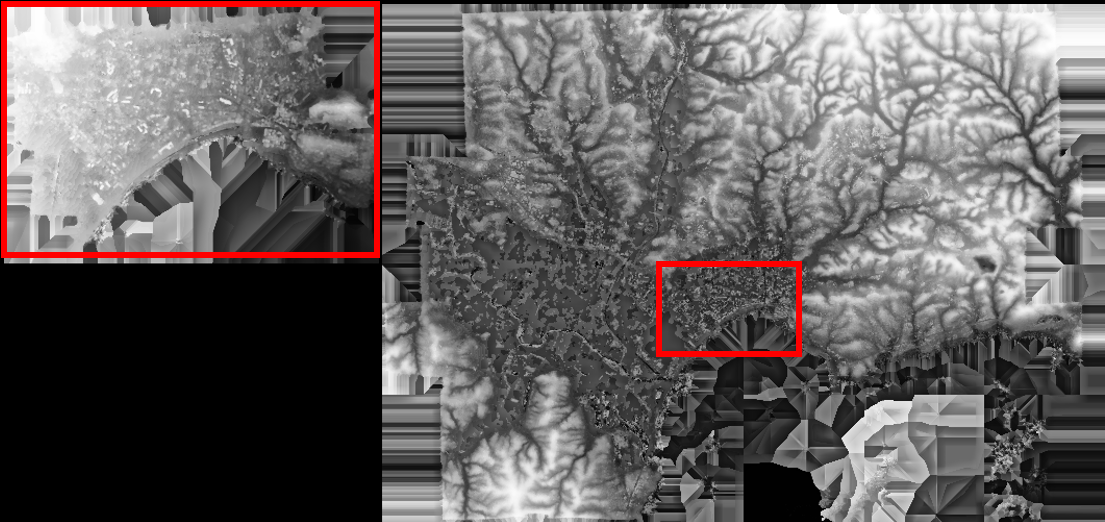
\includegraphics[width=7.5cm]{images/Chapitre3/MEC-Malt_Tapas_1970_MEC-Malt_2014.png}
			\end{minipage}%
		}
		\subfigure[Number of recovered matches]{
			\begin{minipage}[t]{0.48\linewidth}
				\centering
				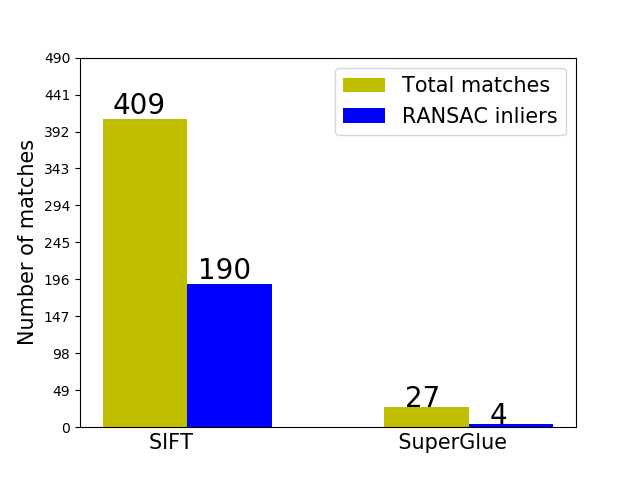
\includegraphics[width=4.8cm]{images/appendix2/PlotCurves_TileTest-MEC-Malt_Tapas_1970_MEC-Malt_2014.png}
			\end{minipage}%
		}
		\subfigure[$SuperGlue_{tiling}^{RANSAC Inliers}$]{
			\begin{minipage}[t]{0.48\linewidth}
				\centering
				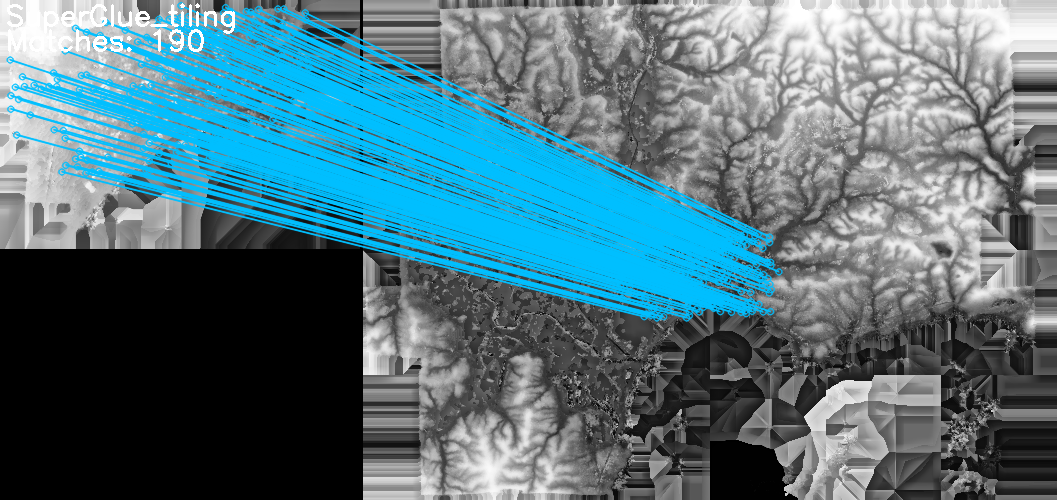
\includegraphics[width=6cm]{images/appendix2/Homol-SubPatch_R270-2DRANSAC_MEC-Malt_Tapas_1970_MEC-Malt_2014.png}
			\end{minipage}%
		}
		\subfigure[$SuperGlue_{orig}^{TotalMatches}$]{
			\begin{minipage}[t]{0.48\linewidth}
				\centering
				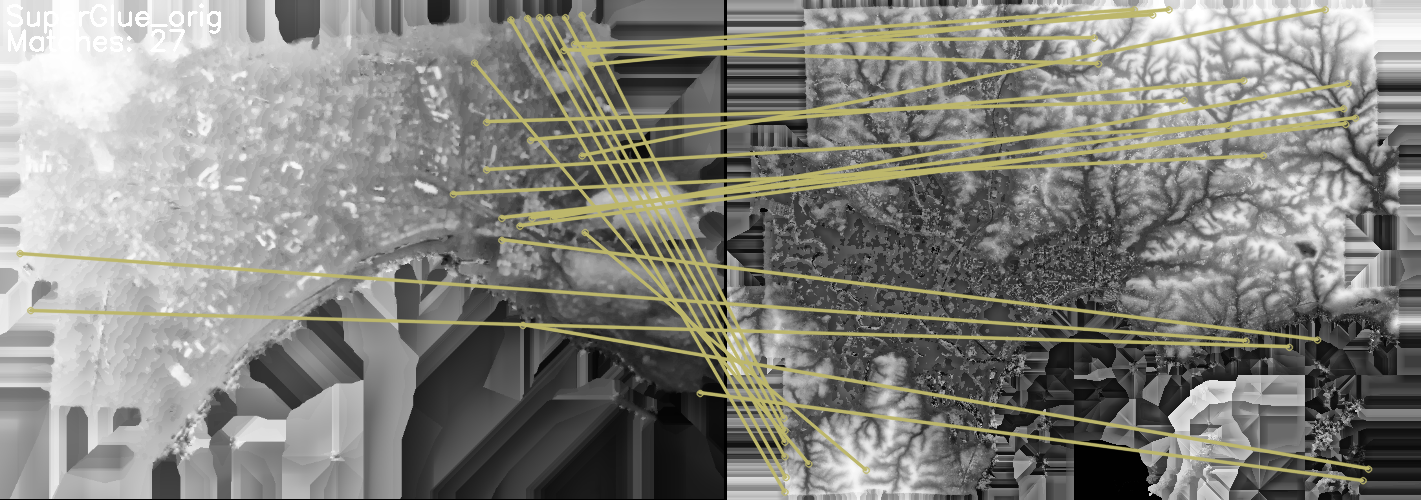
\includegraphics[width=6cm]{images/appendix2/Homol-SuperGlue_MEC-Malt_Tapas_1970_MEC-Malt_2014.png}
			\end{minipage}%
		}
		\caption{Comparison between $SuperGlue_{tiling}$ and $SuperGlue_{orig}$ on \ac{DSM}s from Fr{\'e}jus 1970 and 2014 individually. (a) \ac{DSM}s to be matched, with red rectangles indicating the overlapping zone. (b) Numbers of total matches and RANSAC inliers of $SuperGlue_{tiling}$ and $SuperGlue_{orig}$. (c) Visualization of RANSAC inliers based on $SuperGlue_{tiling}$. (d)Visualization of total matches based on $SuperGlue_{orig}$.}
		\label{MatchDSM}
	\end{center}
\end{figure*} 

In general, $SuperGlue_{tiling}$ is able to recover enough good matches with high inlier ratio to guarantee stability in RANSAC, while $SuperGlue_{orig}$ fails to find any correct matches. In other words, our \textit{one-to-many tiling scheme} improves the performance of SuperGlue significantly.% for variants $SuperGlue_{Ortho}$ and $SuperGlue_{DSM}$.\\

\subsection{Use case of matching guided by 2D similarity transformation}
\label{inputHomography}
In this section we show an example where using 2D similarity model to guide matching is the only possible approach. 
The image pair to be matched is taken at the same time in Hofsjökull (c.f., Figure \ref{Matchresult}(a)). The overlapping zone is indicated with red rectangles. As can be seen, the area is fully covered with snow. It is extremely challenging to be matched as the whole image is weakly textured. \zll{However, the details revealed in the purple squares demonstrated that there are still some helpful information available.} 
%, both SIFT and SuperGlue failed on them. By inputting a set of 2D similarity transformation parameters, we can narrow down the search space and therefore successfully recovered a large number of good matches. The 2D similarity transformation parameters can be estimated by manually measuring 2 matches. Even though it involves manual operation, the work load is negligible and worthy.
We compare the performance of \textit{state-of-the-art} matching methods: (1) SIFT and (2) SuperGlue, as well as our matching strategy: (3) SIFT under the guidance of 2D similarity transformation model followed by RANSAC to remove outliers. 
No less than two matches are required to estimate the 2D similarity transformation parameters. 
\zll{In this particular case we need to measure 2 matching points manually. In less challenging scenarios one can use automated feature extractors for that purpose.\\}
\par
For each keypoint in the master image, our strategy uses 2D similarity transformation model to predict a location in the secondary image and search only its neighborhood of a circle with a radius S (in our experiment, S is set to be 45, 30 and 15 pixels respectively) to reduce ambiguity.\\
%The Hofsjökull dataset, with the details elaborated in Section~\ref{chap:ApplicationsAndDatasets}, is chosen to perform the experiment.
Figure~\ref{Matchresult}(b-f) demonstrates the matching results of SIFT, SuperGlue and our matching strategy. As can be seen, SIFT and SuperGlue fail to find any correct matches, while our strategy obtains a large number of good matches with negligible manual labor. The number of matches increases as the search radius S changes from 45 to 15, which is reasonable due to decrease of ambiguity. However, false matches are introduced when the radius is too small (c.f., Figure~\ref{Matchresult}(f)). The best balance is achieved with S set to be 30 pixels (c.f., Figure~\ref{Matchresult}(e)).\\
%. Even though it involves manual operation, the work load is negligible and worthy
\begin{figure*}[htbp]
	\begin{center}
		\subfigure[Overlapping zone with details]{
			\begin{minipage}[t]{1\linewidth}
				\centering
				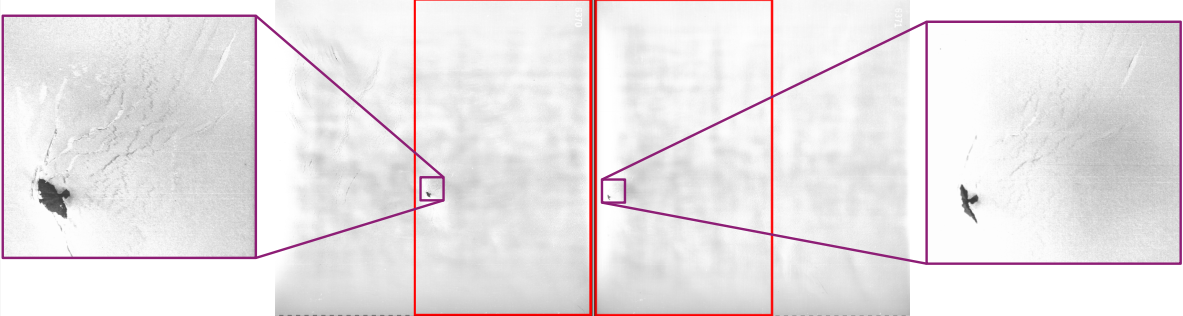
\includegraphics[width=13cm]{images/appendix3/3-6370_crp_8Bits_3-6371_crp_8Bits.png}
			\end{minipage}%
		}
		\subfigure[SIFT]{
			\begin{minipage}[t]{0.48\linewidth}
				\centering
				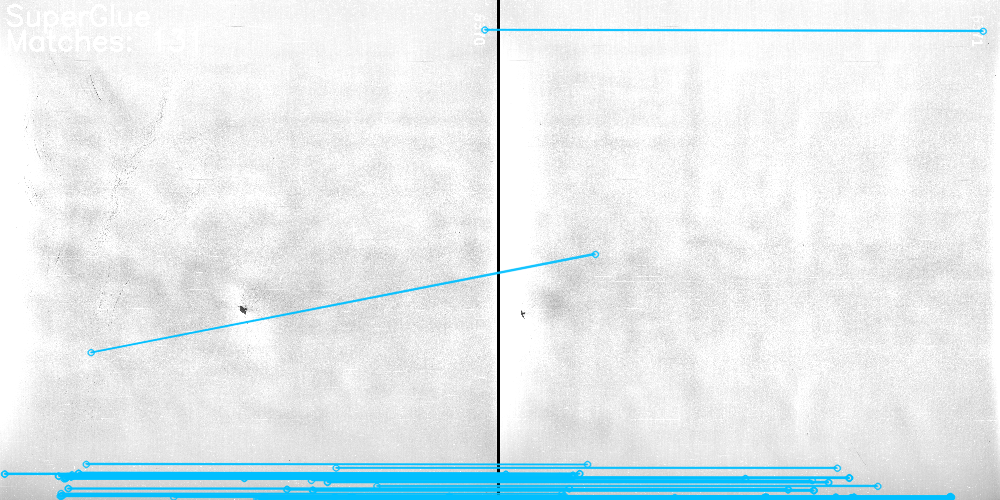
\includegraphics[width=6.3cm]{images/appendix3/Homol-TXT_3-6370_crp_8Bits_3-6371_crp_8Bits.png}
			\end{minipage}%
		}
		\subfigure[SuperGlue]{
			\begin{minipage}[t]{0.48\linewidth}
				\centering
				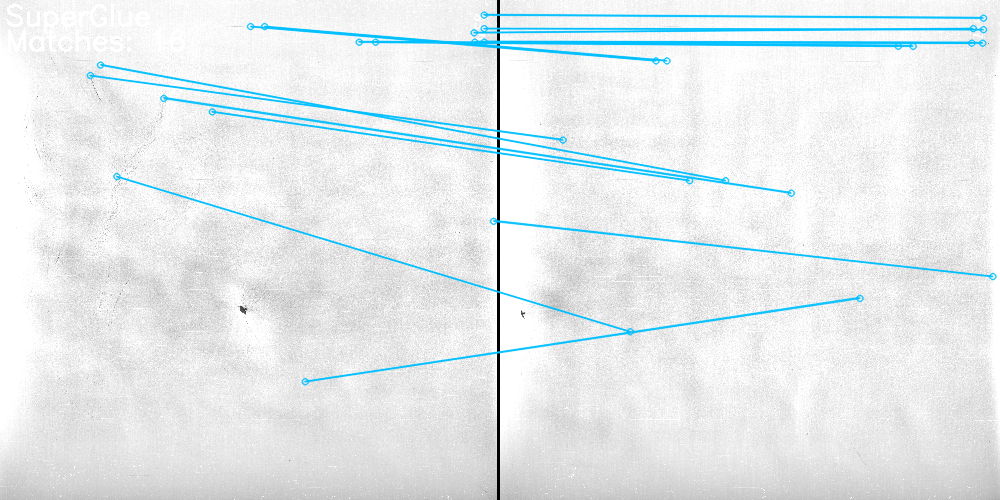
\includegraphics[width=6.3cm]{images/appendix3/Homol-SuperGlue_3-6370_crp_8Bits_3-6371_crp_8Bits.png}
			\end{minipage}%
		}
		\subfigure[Guided SIFT (S=45)]{
			\begin{minipage}[t]{0.31\linewidth}
				\centering
				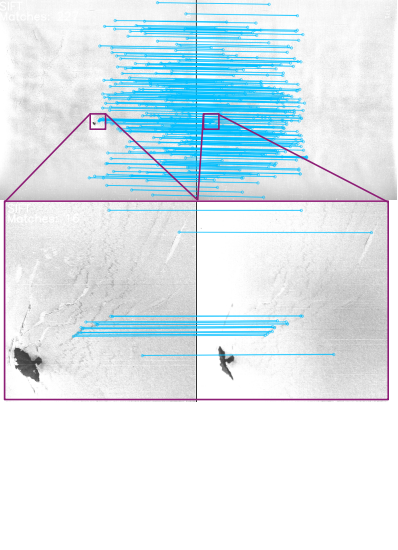
\includegraphics[width=4.5cm]{images/appendix3/Homol-SIFT2Step-2DRANSAC_3-6370_crp_8Bits_3-6371_crp_8Bits-45.png}
			\end{minipage}%
		}
		\subfigure[Guided SIFT (S=30)]{
			\begin{minipage}[t]{0.31\linewidth}
				\centering
				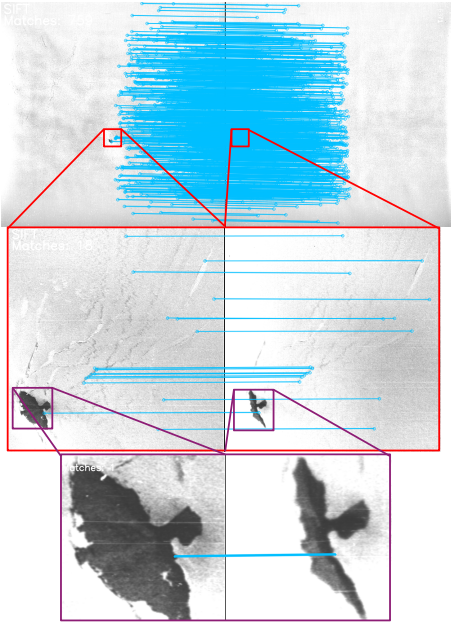
\includegraphics[width=4.5cm]{images/appendix3/Homol-SIFT2Step-2DRANSAC_3-6370_crp_8Bits_3-6371_crp_8Bits-30.png}
			\end{minipage}%
		}
		\subfigure[Guided SIFT (S=15)]{
			\begin{minipage}[t]{0.31\linewidth}
				\centering
				\includegraphics[width=4.5cm]{images/appendix3/Homol-SIFT2Step-2DRANSAC_3-6370_crp_8Bits_3-6371_crp_8Bits-15.png}
			\end{minipage}%
		}
		\caption{Matching results of an intra-epoch image pair from dataset Hofsjökull. (a) Image pairs to be matched, with red rectangles indicating the overlapping zone. \zll{Details are revealed in purple squares.} (b) and (c) are matches recovered by SIFT and SuperGlue individually. (d-f) displays matches found by our matching strategy with search radius set to be 45, 30 and 15 pixels individually, with purple squares indicating the details.}
		\label{Matchresult}
	\end{center}
\end{figure*} 

%\begin{figure*}[htbp]
%	\begin{center}
%		\subfigure[SIFT]{
%			\begin{minipage}[t]{0.48\linewidth}
%				\centering
%				\includegraphics[width=6.3cm]{images/appendix3/Homol-SIFT2Step-2DRANSAC_3-6370_crp_8Bits_3-6371_crp_8Bits-15.png}
%			\end{minipage}%
%		}
%		\subfigure[SuperGlue]{
%			\begin{minipage}[t]{0.48\linewidth}
%				\centering
%				\includegraphics[width=6.3cm]{images/appendix3/Homol-SIFT2Step-2DRANSAC_3-6370_crp_8Bits_3-6371_crp_8Bits-45.png}
%			\end{minipage}%
%		}
%		\caption{Matching result of image pair from Figure~\ref{Hofsjökull} (e) and (f). (a) and (b) are matches recovered by SIFT and SuperGlue individually. (c) displayed the matches found by our matching strategy, which is achieved by narrowing down the search space under the guidance of 2D similarity transformation model.}
%		\label{MatchresultS}
%	\end{center}
%\end{figure*} 

%Show piled image of each epoch?
\subsection{Comparison of 6 variants}
\label{Comparisonof6variants}
%%(1)Matches visualization\\
%%%inlier ratio (RANSAC and \ac{GT})\\
%%(2)Ground check points\\
%%(3)DoD\\
%For each dataset, we manually measured 3 GCPs well distributed in the block. The application of 3 GCPs is twofold:\\
%\begin{itemize}
%    \item Based on the GCPs, a 3D Helmert transformation model between each free epoch and the reference epoch is built to obtain the \ac{GT} co-registered orientations.
%    \item GCPs are also treated as ground check points to evaluate the co-registered orientations calculated by our methods.
%\end{itemize}
%%as check points to evaluate the roughly co-registered orientations resulted by 6 methods:\\
In order to evaluate the results of the 6 variants qualitatively and quantitatively, the following criteria are applied:\\
\begin{enumerate}
    \item \textbf{Matches visualization}. The numbers of (1) total matches (i.e., matches before RANSAC) as well as (2) RANSAC inliers (matches that survived RANSAC) are displayed together in bar charts; in the meantime, the RANSAC inliers are visualized and demonstrated, from which we can tell whether the variants succeeded or failed.
%    \item Ground check points: the co-registered orientations calculated by our methods would be used to triangulate the ground check points and the coordinate differences \textcolor{red}{(explain the diff means the mean diff of x, y and z)} will be displayed. The better the epochs co-register, the smaller the difference is.
    \item \textbf{\ac{DoD}}. For the variants that succeeded, we use the resulted orientations in the same frame to calculate \ac{DSM}s in order to generate \ac{DoD}. The visualization of \ac{DoD} as well as the statistical information are displayed.
    %Ideally the DoD should only display the scene changes. If the dome effect appears, it indicates the systematic errors caused by poorly estimated camera parameters.   
\end{enumerate}

%\subsection{Comparison}
%分三部分分别展示3组数据的结果
%3*2 methods:
%1张表表示6种方法的(1)和(2),1张大图放6种方法的DoD, inlier tie pt图(R3D, \ac{DSM}, ortho各3张(无点图,SIFT点图,SpG点图))
%As the \ac{DoD}s showed similar pattern, we only show the results of 2 sets of datasets (i.e., Fr{\'e}jus and Alberona), as the former represents challenging cases with drastic scene changes and the latter stands for general case, and we move the \ac{DoD}s of Kobe as well as Pezenas to Section~\ref{sec:PreciseDoD} to keep the current section tidy.\\

As the results reveal similar pattern on different datasets, for the sake of simplicity, we only show the results of 2 sets of datasets (i.e., Fr{\'e}jus and Alberona), as the former represents challenging case with drastic scene changes and the latter stands for general case, and we move the results of Kobe as well as Pezenas to Appendix~\ref{chap:appendixA} to keep the current section tidy.\\

%\subsubsection{Matches visualization}
\paragraph{Matches visualization.}
\label{sec:MatchVizMainBody}
For each dataset, each free epoch $E_f$ is matched with reference epoch $E_r$ with 6 variants (i.e., \ding{172} $SIFT_{ImgPairs}$, \ding{173} $SuperGlue_{ImgPairs}$, \ding{174} $SIFT_{Ortho}$, \ding{175} $SuperGlue_{Ortho}$, \ding{176} $SIFT_{DSM}$ and \ding{177} $SuperGlue_{DSM}$), the matches are visualized and displayed together for comparison. In Table~\ref{succeedorfail} we display whether the 6 variants succeeded or failed on all the datasets.\\


\begin{table}[htbp]
	\centering
	\begin{tabular}{||l|c|c|c|c|c|c||}\hline
		&\multicolumn{2}{c|}{ImgPairs} &\multicolumn{2}{c|}{Ortho} &\multicolumn{2}{c|}{\ac{DSM}}\\\hline
		& SIFT & SuperGlue & SIFT & SuperGlue & SIFT & SuperGlue \\\hline\hline
		$Frejus_{2014}^{1954}$ &  Fail  &  \textbf{Succeed}  &  Fail  &  \textbf{Succeed}  &  \textbf{Succeed}  &  \textbf{Succeed} \\
		$Frejus_{2014}^{1966}$ &  Fail  &  \textbf{Succeed}  &  Fail  &  \textbf{Succeed}  &  \textbf{Succeed}  &  \textbf{Succeed} \\
		$Frejus_{2014}^{1970}$ &  Fail  &  \textbf{Succeed}  &  Fail  &  \textbf{Succeed}  &  \textbf{Succeed}  &  \textbf{Succeed} \\\hline
		$Pezenas_{2015}^{1971}$ &  \textbf{Succeed}  &  \textbf{Succeed}  &  \textbf{Succeed}  &  \textbf{Succeed}  &  \textbf{Succeed}  &  \textbf{Succeed} \\
		$Pezenas_{2015}^{1981}$ &  \textbf{Succeed}  &  \textbf{Succeed}  &  \textbf{Succeed}  &  \textbf{Succeed}  &  \textbf{Succeed}  &  \textbf{Succeed} \\\hline
		$Pezenas_{2014(Satellite)}^{1971}$ & / & / &  Fail  &  Fail  &  \textbf{Succeed}  &  \textbf{Succeed} \\
		$Pezenas_{2014(Satellite)}^{1981}$ & / & / &  Fail  &  \textbf{Succeed}  &  \textbf{Succeed}  &  \textbf{Succeed} \\\hline
		$Kobe_{1995}^{1991}$ &  Fail  &  \textbf{Succeed}  &  Fail  &  \textbf{Succeed}  &  \textbf{Succeed}  &  \textbf{Succeed} \\\hline
		$Alberona_{2003}^{1954}$ &  Fail  &  \textbf{Succeed}  &  Fail  &  \textbf{Succeed}  &  \textbf{Succeed}  &  \textbf{Succeed} \\\hline
	\end{tabular}
	\caption{Demonstration of 6 variants succeeding or failing on each dataset.}
	\label{succeedorfail}
\end{table}


%%\begin{enumerate}
%	%\item 
For Fr{\'e}jus, the reference epoch $E_r$ is 2014, the matches visualizations between free epochs $E_f$ (i.e., epoch 1954, 1966 and 1970) and $E_r$ are displayed in Figure~\ref{MatchVizFrejus1954DSM}, ~\ref{MatchVizFrejus1966DSM} and ~\ref{MatchVizFrejus1970DSM} individually. 
%As can be seen, for all 3 free epochs:\\
%\begin{itemize}
%	\item[-] $SIFT_{ImgPairs}$ and $SIFT_{Ortho}$ failed to recover correct matches. It is reasonable as extreme scene changes are present in Fr{\'e}jus, yet SIFT is not sufficiently invariant over time by its very nature.
%	\item[-] $SIFT_{DSM}$ found several good matches after RANSAC, thanks to stable information on DSMs. However, the inlier ratio is dangerously low (around 1\%), it makes the RANSAC procedure unstable and the rough co-registration result inferior.
%	\item[-] $SuperGlue_{ImgPairs}$, $SuperGlue_{Ortho}$ and $SuperGlue_{DSM}$ succeeded to find enough good matches, with the inlier ratios ranging from 3.3\% to 46.5\%. In general, the inlier ratios raise from $SuperGlue_{ImgPairs}$ to $SuperGlue_{Ortho}$ then to $SuperGlue_{DSM}$.
%\end{itemize}
For Alberona, the reference epoch $E_r$ is 2003, the matches visualizations between free epoch $E_f$ (i.e., epoch 1954) and $E_r$ are displayed in Figure~\ref{MatchVizAlberona1954DSM}. %As can be seen:\\
%	\begin{itemize}
%		\item[-] $SIFT_{ImgPairs}$ and $SIFT_{Ortho}$ failed, while $SIFT_{DSM}$ recovered a lot of good matches with inlier ratio reached 49.8\% in RANSAC.
%		\item[-] $SuperGlue_{ImgPairs}$, $SuperGlue_{Ortho}$ and $SuperGlue_{DSM}$ successfully found good matches with RANSAC inlier ratio of 27.0\%, 83.3\% and 90.3\% individually.
%	\end{itemize}
%%\end{enumerate}
%
%In conclusion:\\
%\begin{itemize}
%	\item SuperGlue is more robust than SIFT for all the 3 pipelines (\textit{ImgPairs}, \textit{Ortho}, \textit{DSM}), leading to higher inlier ratio in RANSAC.
%	\item Pipeline \textit{DSM} gets better performance than \textit{ImgPairs} and \textit{Ortho}.
%	\item Pipeline \textit{ImgPairs} often gets more matches as they have higher resolution than \textit{Ortho} and \textit{DSM}, which leads to lower efficiency in the meantime. %However the performance is not necessarily better.
%\end{itemize}

%The same pattern appears for the datasets Fr{\'e}jus, Pezenas and Kobe. For more details please refer to section~\ref{sec:matchViz}.

%Generally speaking, \textit{DSM} gets better performance than \textit{ImgPairs} and \textit{Ortho}. The result of \textit{ImgPairs} is not bad on 
%总结:变化不大时,ImgPairs效果最好
%ImgPairs效率最低


\begin{figure*}[htbp]
	\begin{center}
		\subfigure[Image pairs (19$\times$33 pairs)]{
			\begin{minipage}[t]{0.48\linewidth}
				\centering
				\includegraphics[width=6.8cm]{images/Chapitre3/Pseudo-Ortho-MEC-Malt_Tapas_1954_Ortho-MEC-Malt_2014.png}
			\end{minipage}%
		}
		\subfigure[Number of recovered matches(\textit{ImgPairs})]{
			\begin{minipage}[t]{0.48\linewidth}
				\centering
				\includegraphics[width=3.5cm,trim=0 20 0 38,clip]{images/Chapitre3/PlotCurves_Pseudo-Ortho-MEC-Malt_Tapas_1954_Ortho-MEC-Malt_2014.png}
			\end{minipage}%
		}
		\subfigure[$SIFT_{ImgPairs}^{RANSAC Inliers}$]{
			\begin{minipage}[t]{0.48\linewidth}
				\centering
				\includegraphics[width=6.8cm]{images/Chapitre3/Pseudo-Homol-SIFT2Step_1954-2014-Rough-2DRANSAC-GlobalR3D-PileImg_Ortho-MEC-Malt_Tapas_1954_Ortho-MEC-Malt_2014.png}
			\end{minipage}%
		}
		\subfigure[$SuperGlue_{ImgPairs}^{RANSAC Inliers}$]{
			\begin{minipage}[t]{0.48\linewidth}
				\centering
				\includegraphics[width=6.8cm]{images/Chapitre3/Pseudo-Homol-SuperGlue_1954-2014-GlobalR3D-PileImg_Ortho-MEC-Malt_Tapas_1954_Ortho-MEC-Malt_2014.png}
			\end{minipage}%
		}
		%        \caption{Result of matching image pairs (i.e., \textit{ImgPairs}) of Fr{\'e}jus 1954 and 2014. (a) Image pairs to be matched, with red rectangles indicating the overlapping zone. (b) Numbers of total matches and RANSAC inliers of both SIFT and SuperGlue. (c) Visualization of RANSAC inliers based on SIFT. (d) Visualization of RANSAC inliers based on SuperGlue.}
		%        \label{MatchVizFrejus1954ImgPairs}
		%    \end{center}
		%\end{figure*} 
		%
		%
		%
		%\begin{figure*}[htbp]
		%    \begin{center}
		\subfigure[Orthophotos]{
			\begin{minipage}[t]{0.48\linewidth}
				\centering
				\includegraphics[width=6.8cm]{images/Chapitre3/Ortho-MEC-Malt_Tapas_1954_Ortho-MEC-Malt_2014.png}
			\end{minipage}%
		}
		\subfigure[Number of recovered matches(\textit{Ortho})]{
			\begin{minipage}[t]{0.48\linewidth}
				\centering
				\includegraphics[width=3.5cm,trim=0 20 0 38,clip]{images/Chapitre3/PlotCurves_Ortho-MEC-Malt_Tapas_1954_Ortho-MEC-Malt_2014.png}
			\end{minipage}%
		}
		\subfigure[$SIFT_{Ortho}^{RANSAC Inliers}$]{
			\begin{minipage}[t]{0.48\linewidth}
				\centering
				\includegraphics[width=6.8cm]{images/Chapitre3/Homol-SIFT2Step-Rough-2DRANSAC_Ortho-MEC-Malt_Tapas_1954_Ortho-MEC-Malt_2014.png}
			\end{minipage}%
		}
		\subfigure[$SuperGlue_{Ortho}^{RANSAC Inliers}$]{
			\begin{minipage}[t]{0.48\linewidth}
				\centering
				\includegraphics[width=6.8cm]{images/Chapitre3/Homol-SubPatch_R270-2DRANSAC_Ortho-MEC-Malt_Tapas_1954_Ortho-MEC-Malt_2014.png}
			\end{minipage}%
		}
		%        \caption{Result of matching orthophotos (i.e., \textit{Ortho}) of Fr{\'e}jus 1954 and 2014. (a) Orthophotos to be matched, with red rectangles indicating the overlapping zone. (b) Numbers of total matches and RANSAC inliers of both SIFT and SuperGlue. (c) Visualization of RANSAC inliers based on SIFT. (d) Visualization of RANSAC inliers based on SuperGlue.}
		%        \label{MatchVizFrejus1954Ortho}
		%    \end{center}
		%\end{figure*} 
		%
		%\begin{figure*}[htbp]
		%    \begin{center}
		\subfigure[\ac{DSM}s]{
			\begin{minipage}[t]{0.48\linewidth}
				\centering
				\includegraphics[width=6.8cm]{images/Chapitre3/MEC-Malt_Tapas_1954_MEC-Malt_2014.png}
			\end{minipage}%
		}
		\subfigure[Number of recovered matches(\textit{DSM})]{
			\begin{minipage}[t]{0.48\linewidth}
				\centering
				\includegraphics[width=3.5cm,trim=0 20 0 38,clip]{images/Chapitre3/PlotCurves_MEC-Malt_Tapas_1954_MEC-Malt_2014.png}
			\end{minipage}%
		}
		\subfigure[$SIFT_{DSM}^{RANSAC Inliers}$]{
			\begin{minipage}[t]{0.48\linewidth}
				\centering
				\includegraphics[width=6.8cm]{images/Chapitre3/Homol-SIFT2Step-Rough-2DRANSAC_MEC-Malt_Tapas_1954_MEC-Malt_2014.png}
			\end{minipage}%
		}
		\subfigure[$SuperGlue_{DSM}^{RANSAC Inliers}$]{
			\begin{minipage}[t]{0.48\linewidth}
				\centering
				\includegraphics[width=6.8cm]{images/Chapitre3/Homol-SubPatch_R270-2DRANSAC_MEC-Malt_Tapas_1954_MEC-Malt_2014.png}
			\end{minipage}%
		}
		%\caption{Result of matching DSMs (i.e., \textit{DSM}) of Fr{\'e}jus 1954 and 2014. (a) DSMs to be matched, with red rectangles indicating the overlapping zone. (b) Numbers of total matches and RANSAC inliers of both SIFT and SuperGlue. (c) Visualization of RANSAC inliers based on SIFT. (d) Visualization of RANSAC inliers based on SuperGlue.}
		\caption{Result of \textit{ImgPairs} (a-d), \textit{Ortho} (e-h) and \textit{DSM} (i-l) on matching \textbf{Fr{\'e}jus 1954 and 2014}. (a, e, i) Image pairs/orthophotos/\ac{DSM}s to be matched, with red rectangles indicating the overlapping zone. (b, f, j) Numbers of total matches and RANSAC inliers of both SIFT and SuperGlue on variants \textit{ImgPairs}, \textit{Ortho} and \textit{DSM} individually. (c, g, k) Visualization of RANSAC inliers based on $SIFT_{ImgPairs}$, $SIFT_{Ortho}$ and $SIFT_{DSM}$. (d, h, l) Visualization of RANSAC inliers based on $SuperGlue_{ImgPairs}$, $SuperGlue_{Ortho}$ and $SuperGlue_{DSM}$.}
		\label{MatchVizFrejus1954DSM}
	\end{center}
\end{figure*} 



\begin{figure*}[htbp]
	\begin{center}
		\subfigure[Image pairs (15$\times$33 pairs)]{
			\begin{minipage}[t]{0.48\linewidth}
				\centering
				\includegraphics[width=6.1cm]{images/Chapitre3/Pseudo-Ortho-MEC-Malt_Tapas_1966_Ortho-MEC-Malt_2014.png}
			\end{minipage}%
		}
		\subfigure[Number of recovered matches(\textit{ImgPairs})]{
			\begin{minipage}[t]{0.48\linewidth}
				\centering
				\includegraphics[width=3.5cm,trim=0 20 0 38,clip]{images/Chapitre3/PlotCurves_Pseudo-Ortho-MEC-Malt_Tapas_1966_Ortho-MEC-Malt_2014.png}
			\end{minipage}%
		}
		\subfigure[$SIFT_{ImgPairs}^{RANSAC Inliers}$]{
			\begin{minipage}[t]{0.48\linewidth}
				\centering
				\includegraphics[width=6cm]{images/Chapitre3/Pseudo-Homol-SIFT2Step_1966-2014-Rough-2DRANSAC-GlobalR3D-PileImg_Ortho-MEC-Malt_Tapas_1966_Ortho-MEC-Malt_2014.png}
			\end{minipage}%
		}
		\subfigure[$SuperGlue_{ImgPairs}^{RANSAC Inliers}$]{
			\begin{minipage}[t]{0.48\linewidth}
				\centering
				\includegraphics[width=6cm]{images/Chapitre3/Pseudo-Homol-SuperGlue_1966-2014-GlobalR3D-PileImg_Ortho-MEC-Malt_Tapas_1966_Ortho-MEC-Malt_2014.png}
			\end{minipage}%
		}
		%        \caption{Result of matching image pairs (i.e., \textit{ImgPairs}) of Fr{\'e}jus 1966 and 2014. (a) Image pairs to be matched, with red rectangles indicating the overlapping zone. (b) Numbers of total matches and RANSAC inliers of both SIFT and SuperGlue. (c) Visualization of RANSAC inliers based on SIFT. (d) Visualization of RANSAC inliers based on SuperGlue.}
		%        \label{MatchVizFrejus1966ImgPairs}
		%    \end{center}
		%\end{figure*} 
		%
		%
		%\begin{figure*}[htbp]
		%    \begin{center}
		\subfigure[Orthophotos]{
			\begin{minipage}[t]{0.48\linewidth}
				\centering
				\includegraphics[width=6.1cm]{images/Chapitre3/Ortho-MEC-Malt_Tapas_1966_Ortho-MEC-Malt_2014.png}
			\end{minipage}%
		}
		\subfigure[Number of recovered matches(\textit{Ortho})]{
			\begin{minipage}[t]{0.48\linewidth}
				\centering
				\includegraphics[width=3.5cm,trim=0 20 0 38,clip]{images/Chapitre3/PlotCurves_Ortho-MEC-Malt_Tapas_1966_Ortho-MEC-Malt_2014.png}
			\end{minipage}%
		}
		\subfigure[$SIFT_{Ortho}^{RANSAC Inliers}$]{
			\begin{minipage}[t]{0.48\linewidth}
				\centering
				\includegraphics[width=6cm]{images/Chapitre3/Homol-SIFT2Step-Rough-2DRANSAC_Ortho-MEC-Malt_Tapas_1966_Ortho-MEC-Malt_2014.png}
			\end{minipage}%
		}
		\subfigure[$SuperGlue_{Ortho}^{RANSAC Inliers}$]{
			\begin{minipage}[t]{0.48\linewidth}
				\centering
				\includegraphics[width=6cm]{images/Chapitre3/Homol-SubPatch_R270-2DRANSAC_Ortho-MEC-Malt_Tapas_1966_Ortho-MEC-Malt_2014.png}
			\end{minipage}%
		}
		%        \caption{Result of matching orthophotos (i.e., \textit{Ortho}) of Fr{\'e}jus 1966 and 2014. (a) Orthophotos to be matched, with red rectangles indicating the overlapping zone. (b) Numbers of total matches and RANSAC inliers of both SIFT and SuperGlue. (c) Visualization of RANSAC inliers based on SIFT. (d) Visualization of RANSAC inliers based on SuperGlue.}
		%        \label{MatchVizFrejus1966Ortho}
		%    \end{center}
		%\end{figure*} 
		%
		%\begin{figure*}[htbp]
		%    \begin{center}
		\subfigure[\ac{DSM}s]{
			\begin{minipage}[t]{0.48\linewidth}
				\centering
				\includegraphics[width=6.1cm]{images/Chapitre3/MEC-Malt_Tapas_1966_MEC-Malt_2014.png}
			\end{minipage}%
		}
		\subfigure[Number of recovered matches(\textit{DSM})]{
			\begin{minipage}[t]{0.48\linewidth}
				\centering
				\includegraphics[width=3.5cm,trim=0 20 0 38,clip]{images/Chapitre3/PlotCurves_MEC-Malt_Tapas_1966_MEC-Malt_2014.png}
			\end{minipage}%
		}
		\subfigure[$SIFT_{DSM}^{RANSAC Inliers}$]{
			\begin{minipage}[t]{0.48\linewidth}
				\centering
				\includegraphics[width=6cm]{images/Chapitre3/Homol-SIFT2Step-Rough-2DRANSAC_MEC-Malt_Tapas_1966_MEC-Malt_2014.png}
			\end{minipage}%
		}
		\subfigure[$SuperGlue_{DSM}^{RANSAC Inliers}$]{
			\begin{minipage}[t]{0.48\linewidth}
				\centering
				\includegraphics[width=6cm]{images/Chapitre3/Homol-SubPatch_R270-2DRANSAC_MEC-Malt_Tapas_1966_MEC-Malt_2014.png}
			\end{minipage}%
		}
		%\caption{Result of matching DSMs (i.e., \textit{DSM}) of Fr{\'e}jus 1966 and 2014. (a) DSMs to be matched, with red rectangles indicating the overlapping zone. (b) Numbers of total matches and RANSAC inliers of both SIFT and SuperGlue. (c) Visualization of RANSAC inliers based on SIFT. (d) Visualization of RANSAC inliers based on SuperGlue.}
		%\caption{{\small Result of \textit{ImgPairs}, \textit{Ortho} and \textit{DSM} on Fr{\'e}jus 1966 and 2014. (a, e, i) Image pairs/orthophotos/DSMs to be matched, with red rectangles indicating the overlapping zone. (b, f, j) Numbers of total matches and RANSAC inliers of both SIFT and SuperGlue on variants \textit{ImgPairs}, \textit{Ortho} and \textit{DSM} individually. (c, g, k) Visualization of RANSAC inliers based on $SIFT_{ImgPairs}$, $SIFT_{Ortho}$ and $SIFT_{DSM}$. (d, h, l) Visualization of RANSAC inliers based on $SuperGlue_{ImgPairs}$, $SuperGlue_{Ortho}$ and $SuperGlue_{DSM}$.}}
		\caption{Result of \textit{ImgPairs} (a-d), \textit{Ortho} (e-h) and \textit{DSM} (i-l) on matching \textbf{Fr{\'e}jus 1966 and 2014}. (a, e, i) Image pairs/orthophotos/\ac{DSM}s to be matched, with red rectangles indicating the overlapping zone. (b, f, j) Numbers of total matches and RANSAC inliers of both SIFT and SuperGlue on variants \textit{ImgPairs}, \textit{Ortho} and \textit{DSM} individually. (c, g, k) Visualization of RANSAC inliers based on $SIFT_{ImgPairs}$, $SIFT_{Ortho}$ and $SIFT_{DSM}$. (d, h, l) Visualization of RANSAC inliers based on $SuperGlue_{ImgPairs}$, $SuperGlue_{Ortho}$ and $SuperGlue_{DSM}$.}
		\label{MatchVizFrejus1966DSM}
	\end{center}
\end{figure*} 



\begin{figure*}[htbp]
	\begin{center}
		\subfigure[Image pairs (19$\times$33 pairs)]{
			\begin{minipage}[t]{0.48\linewidth}
				\centering
				\includegraphics[width=5.2cm]{images/Chapitre3/Pseudo-Ortho-MEC-Malt_Tapas_1970_Ortho-MEC-Malt_2014.png}
			\end{minipage}%
		}
		\subfigure[Number of recovered matches(\textit{ImgPairs})]{
			\begin{minipage}[t]{0.48\linewidth}
				\centering
				\includegraphics[width=3.5cm,trim=0 20 0 38,clip]{images/Chapitre3/PlotCurves_Pseudo-Ortho-MEC-Malt_Tapas_1970_Ortho-MEC-Malt_2014.png}
			\end{minipage}%
		}
		\subfigure[$SIFT_{ImgPairs}^{RANSAC Inliers}$]{
			\begin{minipage}[t]{0.48\linewidth}
				\centering
				\includegraphics[width=5.7cm]{images/Chapitre3/Pseudo-Homol-SIFT2Step_1970-2014-Rough-2DRANSAC-GlobalR3D-PileImg_Ortho-MEC-Malt_Tapas_1970_Ortho-MEC-Malt_2014.png}
			\end{minipage}%
		}
		\subfigure[$SuperGlue_{ImgPairs}^{RANSAC Inliers}$]{
			\begin{minipage}[t]{0.48\linewidth}
				\centering
				\includegraphics[width=5.7cm]{images/Chapitre3/Pseudo-Homol-SuperGlue_1970-2014-GlobalR3D-PileImg_Ortho-MEC-Malt_Tapas_1970_Ortho-MEC-Malt_2014.png}
			\end{minipage}%
		}
		%        \caption{Result of matching image pairs (i.e., \textit{ImgPairs}) of Fr{\'e}jus 1970 and 2014. (a) Image pairs to be matched, with red rectangles indicating the overlapping zone. (b) Numbers of total matches and RANSAC inliers of both SIFT and SuperGlue. (c) Visualization of RANSAC inliers based on SIFT. (d) Visualization of RANSAC inliers based on SuperGlue.}
		%        \label{MatchVizFrejus1970ImgPairs}
		%    \end{center}
		%\end{figure*} 
		%
		%\begin{figure*}[htbp]
		%    \begin{center}
		\subfigure[Orthophotos]{
			\begin{minipage}[t]{0.48\linewidth}
				\centering
				\includegraphics[width=5.2cm]{images/Chapitre3/Ortho-MEC-Malt_Tapas_1970_Ortho-MEC-Malt_2014.png}
			\end{minipage}%
		}
		\subfigure[Number of recovered matches(\textit{Ortho})]{
			\begin{minipage}[t]{0.48\linewidth}
				\centering
				\includegraphics[width=3.5cm,trim=0 20 0 38,clip]{images/Chapitre3/PlotCurves_Ortho-MEC-Malt_Tapas_1970_Ortho-MEC-Malt_2014.png}
			\end{minipage}%
		}
		\subfigure[$SIFT_{Ortho}^{RANSAC Inliers}$]{
			\begin{minipage}[t]{0.48\linewidth}
				\centering
				\includegraphics[width=5.7cm]{images/Chapitre3/Homol-SIFT2Step-Rough-2DRANSAC_Ortho-MEC-Malt_Tapas_1970_Ortho-MEC-Malt_2014.png}
			\end{minipage}%
		}
		\subfigure[$SuperGlue_{Ortho}^{RANSAC Inliers}$]{
			\begin{minipage}[t]{0.48\linewidth}
				\centering
				\includegraphics[width=5.7cm]{images/Chapitre3/Homol-SubPatch_R270-2DRANSAC_Ortho-MEC-Malt_Tapas_1970_Ortho-MEC-Malt_2014.png}
			\end{minipage}%
		}
		%        \caption{Result of matching orthophotos (i.e., \textit{Ortho}) of Fr{\'e}jus 1970 and 2014. (a) Orthophotos to be matched, with red rectangles indicating the overlapping zone. (b) Numbers of total matches and RANSAC inliers of both SIFT and SuperGlue. (c) Visualization of RANSAC inliers based on SIFT. (d) Visualization of RANSAC inliers based on SuperGlue.}
		%        \label{MatchVizFrejus1970Ortho}
		%    \end{center}
		%\end{figure*} 
		%
		%\begin{figure*}[htbp]
		%    \begin{center}
		\subfigure[\ac{DSM}s]{
			\begin{minipage}[t]{0.48\linewidth}
				\centering
				\includegraphics[width=5.2cm]{images/Chapitre3/MEC-Malt_Tapas_1970_MEC-Malt_2014.png}
			\end{minipage}%
		}
		\subfigure[Number of recovered matches(\textit{DSM})]{
			\begin{minipage}[t]{0.48\linewidth}
				\centering
				\includegraphics[width=3.5cm,trim=0 20 0 38,clip]{images/Chapitre3/PlotCurves_MEC-Malt_Tapas_1970_MEC-Malt_2014.png}
			\end{minipage}%
		}
		\subfigure[$SIFT_{DSM}^{RANSAC Inliers}$]{
			\begin{minipage}[t]{0.48\linewidth}
				\centering
				\includegraphics[width=5.7cm]{images/Chapitre3/Homol-SIFT2Step-Rough-2DRANSAC_MEC-Malt_Tapas_1970_MEC-Malt_2014.png}
			\end{minipage}%
		}
		\subfigure[$SuperGlue_{DSM}^{RANSAC Inliers}$]{
			\begin{minipage}[t]{0.48\linewidth}
				\centering
				\includegraphics[width=5.7cm]{images/Chapitre3/Homol-SubPatch_R270-2DRANSAC_MEC-Malt_Tapas_1970_MEC-Malt_2014.png}
			\end{minipage}%
		}
		%\caption{Result of matching DSMs (i.e., \textit{DSM}) of Fr{\'e}jus 1970 and 2014. (a) DSMs to be matched, with red rectangles indicating the overlapping zone. (b) Numbers of total matches and RANSAC inliers of both SIFT and SuperGlue. (c) Visualization of RANSAC inliers based on SIFT. (d) Visualization of RANSAC inliers based on SuperGlue.}
		%\caption{{\small Result of \textit{ImgPairs}, \textit{Ortho} and \textit{DSM} on Fr{\'e}jus 1970 and 2014. (a, e, i) image pairs/orthophotos/DSMs to be matched, with red rectangles indicating the overlapping zone. (b, f, j) Numbers of total matches and RANSAC inliers of both SIFT and SuperGlue on variants \textit{ImgPairs}, \textit{Ortho} and \textit{DSM} individually. (c, g, k) Visualization of RANSAC inliers based on $SIFT_{ImgPairs}$, $SIFT_{Ortho}$ and $SIFT_{DSM}$. (d, h, l) Visualization of RANSAC inliers based on $SuperGlue_{ImgPairs}$, $SuperGlue_{Ortho}$ and $SuperGlue_{DSM}$.}}
		\caption{Result of \textit{ImgPairs} (a-d), \textit{Ortho} (e-h) and \textit{DSM} (i-l) on matching \textbf{Fr{\'e}jus 1970 and 2014}. (a, e, i) Image pairs/orthophotos/\ac{DSM}s to be matched, with red rectangles indicating the overlapping zone. (b, f, j) Numbers of total matches and RANSAC inliers of both SIFT and SuperGlue on variants \textit{ImgPairs}, \textit{Ortho} and \textit{DSM} individually. (c, g, k) Visualization of RANSAC inliers based on $SIFT_{ImgPairs}$, $SIFT_{Ortho}$ and $SIFT_{DSM}$. (d, h, l) Visualization of RANSAC inliers based on $SuperGlue_{ImgPairs}$, $SuperGlue_{Ortho}$ and $SuperGlue_{DSM}$.}
		\label{MatchVizFrejus1970DSM}
	\end{center}
\end{figure*} 


%%%%%%%%%%%%%%%%%%%%%%%%%%%%%%%%%%%Alberona
\begin{figure*}[htbp]
	\begin{center}
		\subfigure[Image pairs (3$\times$7 pairs)]{
			\begin{minipage}[t]{0.48\linewidth}
				\centering
				\includegraphics[width=4.8cm]{images/Chapitre3/Pseudo-Ortho-MEC-Malt_Tapas_1954_Ortho-MEC-Malt_Tapas_2003.png}
			\end{minipage}%
		}
		\subfigure[Number of recovered matches(\textit{ImgPairs})]{
			\begin{minipage}[t]{0.48\linewidth}
				\centering
				\includegraphics[width=3.5cm,trim=0 20 0 38,clip]{images/Chapitre3/PlotCurves_Pseudo-Ortho-MEC-Malt_Tapas_1954_Ortho-MEC-Malt_Tapas_2003.png}
			\end{minipage}%
		}
		\subfigure[$SIFT_{ImgPairs}^{RANSAC Inliers}$]{
			\begin{minipage}[t]{0.48\linewidth}
				\centering
				\includegraphics[width=4.8cm]{images/Chapitre3/Pseudo-Homol-SIFT2Step_1954-2003-Rough-2DRANSAC-GlobalR3D-PileImg_Ortho-MEC-Malt_Tapas_1954_Ortho-MEC-Malt_Tapas_2003.png}
			\end{minipage}%
		}
		\subfigure[$SuperGlue_{ImgPairs}^{RANSAC Inliers}$]{
			\begin{minipage}[t]{0.48\linewidth}
				\centering
				\includegraphics[width=4.8cm]{images/Chapitre3/Pseudo-Homol-SuperGlue_1954-2003-GlobalR3D-PileImg_Ortho-MEC-Malt_Tapas_1954_Ortho-MEC-Malt_Tapas_2003.png}
			\end{minipage}%
		}
		%        \caption{Result of matching image pairs (i.e., \textit{ImgPairs}) of Fr{\'e}jus 1954 and 2014. (a) Image pairs to be matched, with red rectangles indicating the overlapping zone. (b) Numbers of total matches and RANSAC inliers of both SIFT and SuperGlue. (c) Visualization of RANSAC inliers based on SIFT. (d) Visualization of RANSAC inliers based on SuperGlue.}
		%        \label{MatchVizFrejus1954ImgPairs}
		%    \end{center}
		%\end{figure*} 
		%
		%
		%
		%\begin{figure*}[htbp]
		%    \begin{center}
		\subfigure[Orthophotos]{
			\begin{minipage}[t]{0.48\linewidth}
				\centering
				\includegraphics[width=4.8cm]{images/Chapitre3/Ortho-MEC-Malt_Tapas_1954_Ortho-MEC-Malt_Tapas_2003.png}
			\end{minipage}%
		}
		\subfigure[Number of recovered matches(\textit{Ortho})]{
			\begin{minipage}[t]{0.48\linewidth}
				\centering
				\includegraphics[width=3.5cm,trim=0 20 0 38,clip]{images/Chapitre3/PlotCurves_Ortho-MEC-Malt_Tapas_1954_Ortho-MEC-Malt_Tapas_2003.png}
			\end{minipage}%
		}
		\subfigure[$SIFT_{Ortho}^{RANSAC Inliers}$]{
			\begin{minipage}[t]{0.48\linewidth}
				\centering
				\includegraphics[width=4.8cm]{images/Chapitre3/Homol-SIFT2Step-Rough-2DRANSAC_Ortho-MEC-Malt_Tapas_1954_Ortho-MEC-Malt_Tapas_2003.png}
			\end{minipage}%
		}
		\subfigure[$SuperGlue_{Ortho}^{RANSAC Inliers}$]{
			\begin{minipage}[t]{0.48\linewidth}
				\centering
				\includegraphics[width=4.8cm]{images/Chapitre3/Homol-SubPatch_R90-2DRANSAC_Ortho-MEC-Malt_Tapas_1954_Ortho-MEC-Malt_Tapas_2003.png}
			\end{minipage}%
		}
		%        \caption{Result of matching orthophotos (i.e., \textit{Ortho}) of Fr{\'e}jus 1954 and 2014. (a) Orthophotos to be matched, with red rectangles indicating the overlapping zone. (b) Numbers of total matches and RANSAC inliers of both SIFT and SuperGlue. (c) Visualization of RANSAC inliers based on SIFT. (d) Visualization of RANSAC inliers based on SuperGlue.}
		%        \label{MatchVizFrejus1954Ortho}
		%    \end{center}
		%\end{figure*} 
		%
		%\begin{figure*}[htbp]
		%    \begin{center}
		\subfigure[\ac{DSM}s]{
			\begin{minipage}[t]{0.48\linewidth}
				\centering
				\includegraphics[width=4.8cm]{images/Chapitre3/MEC-Malt_Tapas_1954_MEC-Malt_Tapas_2003.png}
			\end{minipage}%
		}
		\subfigure[Number of recovered matches(\textit{DSM})]{
			\begin{minipage}[t]{0.48\linewidth}
				\centering
				\includegraphics[width=3.5cm,trim=0 20 0 38,clip]{images/Chapitre3/PlotCurves_MEC-Malt_Tapas_1954_MEC-Malt_Tapas_2003.png}
			\end{minipage}%
		}
		\subfigure[$SIFT_{DSM}^{RANSAC Inliers}$]{
			\begin{minipage}[t]{0.48\linewidth}
				\centering
				\includegraphics[width=4.8cm]{images/Chapitre3/Homol-SIFT2Step-Rough-2DRANSAC_MEC-Malt_Tapas_1954_MEC-Malt_Tapas_2003.png}
			\end{minipage}%
		}
		\subfigure[$SuperGlue_{DSM}^{RANSAC Inliers}$]{
			\begin{minipage}[t]{0.48\linewidth}
				\centering
				\includegraphics[width=4.8cm]{images/Chapitre3/Homol-SubPatch_R90-2DRANSAC_MEC-Malt_Tapas_1954_MEC-Malt_Tapas_2003.png}
			\end{minipage}%
		}
		%\caption{Result of matching DSMs (i.e., \textit{DSM}) of Fr{\'e}jus 1954 and 2014. (a) DSMs to be matched, with red rectangles indicating the overlapping zone. (b) Numbers of total matches and RANSAC inliers of both SIFT and SuperGlue. (c) Visualization of RANSAC inliers based on SIFT. (d) Visualization of RANSAC inliers based on SuperGlue.}
		\caption{Result of \textit{ImgPairs} (a-d), \textit{Ortho} (e-h) and \textit{DSM} (i-l) on matching \textbf{Alberona 1954 and 2003}. (a, e, i) Image pairs/orthophotos/\ac{DSM}s to be matched, with red rectangles indicating the overlapping zone. (b, f, j) Numbers of total matches and RANSAC inliers of both SIFT and SuperGlue on variants \textit{ImgPairs}, \textit{Ortho} and \textit{DSM} individually. (c, g, k) Visualization of RANSAC inliers based on $SIFT_{ImgPairs}$, $SIFT_{Ortho}$ and $SIFT_{DSM}$. (d, h, l) Visualization of RANSAC inliers based on $SuperGlue_{ImgPairs}$, $SuperGlue_{Ortho}$ and $SuperGlue_{DSM}$.}
		\label{MatchVizAlberona1954DSM}
	\end{center}
\end{figure*} 

%As can be seen, 


%\subsubsection{Ground check points}
%
%\begin{table}%[H]
%	\footnotesize
%	\centering
%	\begin{tabular}{|l|cccccc|}\hline
%		&\multicolumn{6}{c}{$|\mu|$ [m]}\\\hline
%		&\multicolumn{2}{c}{ImgPairs} &\multicolumn{2}{c}{Ortho} &\multicolumn{2}{c|}{DSM}\\\hline
%		& SIFT & SuperGlue & SIFT & SuperGlue & SIFT & SuperGlue \\\hline\hline
%		$Frejus_{2014}^{1954}$ & 1380.16 & 29.29 & 2509.13 & 34.84 & 36.58 & \textbf{10.72}\\\hline
%		$Frejus_{2014}^{1966}$ & 1686.56 & 18.15 & 4386.53 & 11.98 & 19.54 & \textbf{10.43}\\\hline
%		$Frejus_{2014}^{1970}$ & 997.83 & 11.09 & 4404.15 & 16.87 & \textbf{8.65} & 10.23\\\hline\hline
%		
%		$Pezenas_{2015}^{1971}$ & 7.03 & ? & 31.68 & 10.85 & 9.15 & \textbf{8.52} \\\hline
%		$Pezenas_{2015}^{1981}$ & \textbf{5.48} & 5.76 & 7.63 & 8.73 & 10.23 & 6.76 \\\hline
%		
%		$Kobe_{1995}^{1991}$ & 369.34 & 3.33 & 68.51 & 4.03 & 4.68 & \textbf{3.31} \\\hline
%	\end{tabular}
%	\caption{Accuracy of 6 sets of co-registered orientations resulting from 6 methods, evaluated on 3 check points uniformly distributed in the block. Absolute average value $|\mu|$ is displayed for each method.}
%	\label{CheckptAcuracy}
%\end{table}

%\subsubsection{\ac{DoD}}
\paragraph{\ac{DoD}.}
\label{sec:RoughDoDMainBody}
According to Table~\ref{succeedorfail}, by applying 6 variants (or 4 variants for satellite images) on each free epoch and the reference epoch, we got 50 testing cases. Among all the cases, there are 37 of them succeeded, which leads to 37 sets of co-registered orientations. For each set of resulted orientations, we use them to calculate \ac{DSM}s in free epoch and reference epoch individually in order to generate \ac{DoD}.
16 sets of \ac{DoD}s belong to Fr{\'e}jus and Alberona therefore are displayed in the current section (Figure~\ref{DoDFrejus} and ~\ref{DoDAlberona}). Their corresponding statistical information is displayed in Table~\ref{RoughDoDStatistic}. The rest 21 sets of \ac{DoD}s are displayed in Appendix \ref{chap:appendixA}. \\

%As the \ac{DoD}s showed similar pattern, we only show the results of 2 sets of datasets (i.e., Fr{\'e}jus and Alberona), as the former represents challenging cases with drastic scene changes and the latter stands for general case, and we move the \ac{DoD}s of Kobe as well as Pezenas to Section~\ref{sec:PreciseDoD} to keep the current section tidy.\\

%The visualizations of \ac{DoD}s for datasets Fr{\'e}jus and Alberona are demonstrated in Figure~\ref{DoDFrejus} and ~\ref{DoDAlberona}. The corresponding statistical information is displayed in Table~\ref{RoughDoDStatistic}.\\
%are demonstrated in Figure~\ref{DoDFrejus}, ~\ref{DoDPezenas}, ~\ref{DoDPezenas-Satellite} and ~\ref{DoDKobe}.
%The statistical information of the 33 \ac{DoD}s are displayed in Table~\ref{DoDStatistic}.\\
%As can be seen, \textit{dome} effect \cite{wackrow2008minimising} is present in all the \ac{DoD}s. %This is because the camera parameters are estimated within the same epoch, therefore the deformation of historical images inevitably leads to unsatisfactory results. 
%This is caused by inaccurately estimated lens distortion parameters.
%It is acceptable for rough co-registration as our goal is only to provide guidance for precise matching. 
%Similar pattern is present in other datasets (Pezenas and Kobe), for more details please refer to Appendix~\ref{sec:RoughDoD}.\\
%
%It is worth noting that the \ac{DoD}s between Fr{\'e}jus 1954 and 2014 based on variant $SIFT_{DSM}$ (i.e., Figure \ref{DoDFrejus} (f)) is accompanied with specifically obvious \textit{dome} effect, with its absolute average value $|\mu|$ reached 8.04m as shown in Table \ref{RoughDoDStatistic}. This is consistent with the results shown in Section \ref{sec:MatchVizMainBody}, as its inlier ratio of matches in the RANSAC procedure is too low to guarantee reliable rough co-registration. According to the absolute average value $|\mu|$ displayed in Table~\ref{RoughDoDStatistic}, variant $SuperGlue_{DSM}$ performed the best for matching Fr{\'e}jus 1954 and 1966 to 2014, where drastic scene changes present, while variants $SuperGlue_{Ortho}$ and $SIFT_{DSM}$ performed the best for less challenging cases (i.e., matching Fr{\'e}jus 1970 to 2014, and Alberona 1954 to 2003). %For the case of matching Fr{\'e}jus 1970 to 2014, as the 2 epochs are with shorter time gap,\\

\begin{figure*}[htbp]
	\begin{center}
		\subfigure[\ac{DoD}$_{Frejus1954}^{SuperGlue_{ImgPairs}}$]{
			\begin{minipage}[t]{0.31\linewidth}
				\centering
				%left, lower, right, up
				\includegraphics[width=3.3cm,trim=680 80 110 220,clip]{images/Chapitre3/DoD1954R3D-SuperGlue.png}
			\end{minipage}%
		}
		\subfigure[\ac{DoD}$_{Frejus1954}^{SuperGlue_{Ortho}}$]{
			\begin{minipage}[t]{0.31\linewidth}
				\centering
				\includegraphics[width=3.3cm,trim=680 80 110 220,clip]{images/Chapitre3/DoD1954Ortho-SuperGlue.png}
			\end{minipage}%
		}
		\subfigure[\ac{DoD}$_{Frejus1954}^{SuperGlue_{DSM}}$]{
			\begin{minipage}[t]{0.31\linewidth}
				\centering
				\includegraphics[width=3.3cm,trim=680 80 110 220,clip]{images/Chapitre3/DoD1954DSM-SuperGlue.png}
			\end{minipage}%
		}
		
		\subfigure[\ac{DoD}$_{Frejus1954}^{SIFT_{ImgPairs}}$]{
			\begin{minipage}[t]{0.31\linewidth}
				\centering
				%left, lower, right, up
				\includegraphics[width=2cm]{images/Chapitre3/NoDoD.png}
			\end{minipage}%
		}
		\subfigure[\ac{DoD}$_{Frejus1954}^{SIFT_{Ortho}}$]{
			\begin{minipage}[t]{0.31\linewidth}
				\centering
				\includegraphics[width=2cm]{images/Chapitre3/NoDoD.png}
			\end{minipage}%
		}
		\subfigure[\ac{DoD}$_{Frejus1954}^{SIFT_{DSM}}$]{
			\begin{minipage}[t]{0.31\linewidth}
				\centering
				\includegraphics[width=3.3cm,trim=680 80 110 220,clip]{images/Chapitre3/DoD1954DSM-SIFT.png}
			\end{minipage}%
		}
		%       \caption{DoDs of SuperGlue and SIFT on dataset Fr{\'e}jus (epoch 1954). The prohibition sign means the corresponding method failed.}
		%       \label{Frejus DoD of SuperGlue}
		%   \end{center}
		%\end{figure*} 
		%
		%\begin{figure*}[htbp]
		%   \begin{center}
		\subfigure[\ac{DoD}$_{Frejus1966}^{SuperGlue_{ImgPairs}}$]{
			\begin{minipage}[t]{0.31\linewidth}
				\centering
				%left, lower, right, up
				\includegraphics[width=3.3cm,trim=740 230 50 380,clip]{images/Chapitre3/DoD1966R3D-SuperGlue.png}
			\end{minipage}%
		}
		\subfigure[\ac{DoD}$_{Frejus1966}^{SuperGlue_{Ortho}}$]{
			\begin{minipage}[t]{0.31\linewidth}
				\centering
				\includegraphics[width=3.3cm,trim=740 230 50 380,clip]{images/Chapitre3/DoD1966Ortho-SuperGlue.png}
			\end{minipage}%
		}
		\subfigure[\ac{DoD}$_{Frejus1966}^{SuperGlue_{DSM}}$]{
			\begin{minipage}[t]{0.31\linewidth}
				\centering
				\includegraphics[width=3.3cm,trim=740 230 50 380,clip]{images/Chapitre3/DoD1966DSM-SuperGlue.png}
			\end{minipage}%
		}
		
		
		\subfigure[\ac{DoD}$_{Frejus1966}^{SIFT_{ImgPairs}}$]{
			\begin{minipage}[t]{0.31\linewidth}
				\centering
				%left, lower, right, up
				\includegraphics[width=2cm]{images/Chapitre3/NoDoD.png}
			\end{minipage}%
		}
		\subfigure[\ac{DoD}$_{Frejus1966}^{SIFT_{Ortho}}$]{
			\begin{minipage}[t]{0.31\linewidth}
				\centering
				\includegraphics[width=2cm]{images/Chapitre3/NoDoD.png}
			\end{minipage}%
		}
		\subfigure[\ac{DoD}$_{Frejus1966}^{SIFT_{DSM}}$]{
			\begin{minipage}[t]{0.31\linewidth}
				\centering
				\includegraphics[width=3.3cm,trim=740 230 50 380,clip]{images/Chapitre3/DoD1966DSM-SIFT.png}
			\end{minipage}%
		}       
		%       \caption{DoDs of SuperGlue and SIFT on dataset Fr{\'e}jus (epoch 1966). The prohibition sign means the corresponding method failed.}
		%\label{Frejus DoD of SuperGlue}
		%\end{center}
		%\end{figure*} 
		%
		%\begin{figure*}[htbp]
		%\begin{center}     
		\subfigure[\ac{DoD}$_{Frejus1970}^{SuperGlue_{ImgPairs}}$]{
			\begin{minipage}[t]{0.31\linewidth}
				\centering
				%left, lower, right, up
				\includegraphics[width=3.3cm,trim=680 180 50 260,clip]{images/Chapitre3/DoD1970R3D-SuperGlue.png}
			\end{minipage}%
		}
		\subfigure[\ac{DoD}$_{Frejus1970}^{SuperGlue_{Ortho}}$]{
			\begin{minipage}[t]{0.31\linewidth}
				\centering
				\includegraphics[width=3.3cm,trim=680 180 50 260,clip]{images/Chapitre3/DoD1970Ortho-SuperGlue.png}
			\end{minipage}%
		}
		\subfigure[\ac{DoD}$_{Frejus1970}^{SuperGlue_{DSM}}$]{
			\begin{minipage}[t]{0.31\linewidth}
				\centering
				\includegraphics[width=3.3cm,trim=680 180 50 260,clip]{images/Chapitre3/DoD1970DSM-SuperGlue.png}
			\end{minipage}%
		}
		
		\subfigure[\ac{DoD}$_{Frejus1970}^{SIFT_{ImgPairs}}$]{
			\begin{minipage}[t]{0.31\linewidth}
				\centering
				%left, lower, right, up
				\includegraphics[width=2cm]{images/Chapitre3/NoDoD.png}
			\end{minipage}%
		}
		\subfigure[\ac{DoD}$_{Frejus1970}^{SIFT_{Ortho}}$]{
			\begin{minipage}[t]{0.31\linewidth}
				\centering
				\includegraphics[width=2cm]{images/Chapitre3/NoDoD.png}
			\end{minipage}%
		}
		\subfigure[\ac{DoD}$_{Frejus1970}^{SIFT_{DSM}}$]{
			\begin{minipage}[t]{0.31\linewidth}
				\centering
				\includegraphics[width=3.3cm,trim=680 180 50 260,clip]{images/Chapitre3/DoD1970DSM-SIFT.png}
			\end{minipage}%
		}
		
		\subfigure[\ac{DoD} legend]{
			\begin{minipage}[t]{1\linewidth}
				\centering
				\includegraphics[width=11cm]{images/Chapitre3/LegendDoD.png}
			\end{minipage}%
		}
		%\caption{DoDs of SuperGlue and SIFT on dataset Fr{\'e}jus (epoch 1970). The prohibition sign means the corresponding method failed.}
		\caption{\ac{DoD}s between free epoch \textbf{Fr{\'e}jus 1954, 1966, 1970} and reference epoch \textbf{2014} with variants $SuperGlue_{ImgPairs}$ (a, g, m), $SuperGlue_{Ortho}$ (b, h, n), $SuperGlue_{DSM}$ (c, i, o), $SIFT_{ImgPairs}$ (d, j, p), $SIFT_{Ortho}$ (e, k, q) and $SIFT_{DSM}$ (f, l, r). The prohibition sign means the corresponding variant failed.}
		\label{DoDFrejus}
	\end{center}
\end{figure*} 

\begin{figure*}[htbp]
	\begin{center}
		\subfigure[\ac{DoD}$_{Alberona}^{SuperGlue_{ImgPairs}}$]{
			\begin{minipage}[t]{0.31\linewidth}
				\centering
				%left, lower, right, up
				\includegraphics[width=4.3cm,trim=870 100 180 180,clip]{images/Chapitre3/DoDAlberona1954R3D-SuperGlue.png}
			\end{minipage}%
		}
		\subfigure[\ac{DoD}$_{Alberona}^{SuperGlue_{Ortho}}$]{
			\begin{minipage}[t]{0.31\linewidth}
				\centering
				\includegraphics[width=4.3cm,trim=870 100 180 180,clip]{images/Chapitre3/DoDAlberona1954Ortho-SuperGlue.png}
			\end{minipage}%
		}
		\subfigure[\ac{DoD}$_{Alberona}^{SuperGlue_{DSM}}$]{
			\begin{minipage}[t]{0.31\linewidth}
				\centering
				\includegraphics[width=4.3cm,trim=870 100 180 180,clip]{images/Chapitre3/DoDAlberona1954DSM-SuperGlue.png}
			\end{minipage}%
		}
		
		\subfigure[\ac{DoD}$_{Alberona}^{SIFT_{ImgPairs}}$]{
			\begin{minipage}[t]{0.31\linewidth}
				\centering
				%left, lower, right, up
				\includegraphics[width=4cm]{images/Chapitre3/NoDoD.png}
			\end{minipage}%
		}
		\subfigure[\ac{DoD}$_{Alberona}^{SIFT_{Ortho}}$]{
			\begin{minipage}[t]{0.31\linewidth}
				\centering
				\includegraphics[width=4cm]{images/Chapitre3/NoDoD.png}
			\end{minipage}%
		}
		\subfigure[\ac{DoD}$_{Alberona}^{SIFT_{DSM}}$]{
			\begin{minipage}[t]{0.31\linewidth}
				\centering
				\includegraphics[width=4.3cm,trim=870 100 180 180,clip]{images/Chapitre3/DoDAlberona1954DSM-SIFT.png}
			\end{minipage}%
		}
		
		\subfigure[\ac{DoD} legend]{
			\begin{minipage}[t]{1\linewidth}
				\centering
				\includegraphics[width=11cm]{images/Chapitre3/LegendDoD.png}
			\end{minipage}%
		}
		\caption{\ac{DoD}s between free epoch \textbf{Alberona 1954} and reference epoch \textbf{2003} with variants $SuperGlue_{ImgPairs}$ (a), $SuperGlue_{Ortho}$ (b), $SuperGlue_{DSM}$ (c), $SIFT_{ImgPairs}$ (d), $SIFT_{Ortho}$ (e) and $SIFT_{DSM}$ (f). The prohibition sign means the corresponding variant failed.}
		\label{DoDAlberona}
	\end{center}
\end{figure*} 


\begin{table}%[H]
	\footnotesize
	\centering
	\begin{tabular}{||l|l|c|c|c||}\hline
		& &$\mu$ [m]&$\sigma$ [m]&$|\mu|$ [m]\\\hline\hline
%		\multirow{6}{*}{$DoD^{Frejus}_{1954-2014}$}
%		&${SuperGlue_{ImgPairs}}$ & 5.70 & 6.32 & 6.62\\
%		&${SuperGlue_{Ortho}}$ & 2.19 & 6.46 & 4.55\\
%		&${SuperGlue_{DSM}}$ & 2.07 & 4.87 & \textbf{3.83} \\
%		&${SIFT_{ImgPairs}}$ & / & / & / \\
%		&${SIFT_{Ortho}}$ & / & / & / \\
%		&${SIFT_{DSM}}$ & 6.92 & 8.47 & 8.04\\\hline
%		
%		\multirow{6}{*}{$DoD^{Frejus}_{1966-2014}$}
%		&${SuperGlue_{ImgPairs}}$ & -1.36 & 3.82 & 2.90\\
%		&${SuperGlue_{Ortho}}$ & -0.37 & 4.22 & 3.01\\
%		&${SuperGlue_{DSM}}$ & -0.46 & 3.77 & \textbf{2.68}\\
%		&${SIFT_{ImgPairs}}$ & / & / & / \\
%		&${SIFT_{Ortho}}$ & / & / & / \\
%		&${SIFT_{DSM}}$ & -1.72 & 4.92 & 3.75\\\hline
%		
%		\multirow{6}{*}{$DoD^{Frejus}_{1970-2014}$}
%		&${SuperGlue_{ImgPairs}}$ & -5.04 & 5.09 & 5.70\\
%		&${SuperGlue_{Ortho}}$ & -2.63 & 5.18 & \textbf{4.39}\\
%		&${SuperGlue_{DSM}}$ & -1.71 & 5.75 & 4.61\\
%		&${SIFT_{ImgPairs}}$ & / & / & / \\
%		&${SIFT_{Ortho}}$ & / & / & / \\
%		&${SIFT_{DSM}}$ & -3.17 & 5.44 & 4.71\\\hline
				\multirow{6}{*}{$DoD^{Frejus}_{1954-2014}$}
				&${SuperGlue_{ImgPairs}}$ & 6.02 & 7.04 & 7.39\\
&${SuperGlue_{Ortho}}$ & 2.55 & 7.31 & 5.29\\
&${SuperGlue_{DSM}}$ & 2.24 & 5.34 & \textbf{4.35}\\
		&${SIFT_{ImgPairs}}$ & / & / & / \\
		&${SIFT_{Ortho}}$ & / & / & / \\
&${SIFT_{DSM}}$ & 6.91 & 8.90 & 8.45\\\hline
		
		\multirow{6}{*}{$DoD^{Frejus}_{1966-2014}$}
				&${SuperGlue_{ImgPairs}}$ & -1.74 & 4.78 & 3.55\\
&${SuperGlue_{Ortho}}$ & -0.69 & 5.11 & 3.59\\
&${SuperGlue_{DSM}}$ & -0.80 & 4.71 & \textbf{3.28}\\
		&${SIFT_{ImgPairs}}$ & / & / & / \\
		&${SIFT_{Ortho}}$ & / & / & / \\
&${SIFT_{DSM}}$ & -2.12 & 5.66 & 4.42\\\hline
		
		\multirow{6}{*}{$DoD^{Frejus}_{1970-2014}$}
				&${SuperGlue_{ImgPairs}}$ & -5.60 & 6.16 & 6.54\\
&${SuperGlue_{Ortho}}$ & -3.34 & 6.50 & 5.48\\
&${SuperGlue_{DSM}}$ & -2.37 & 6.57 & \textbf{5.35}\\
		&${SIFT_{ImgPairs}}$ & / & / & / \\
		&${SIFT_{Ortho}}$ & / & / & / \\
&${SIFT_{DSM}}$ & -3.76 & 6.21 & 5.47\\\hline
		
%		\multirow{6}{*}{$DoD^{Alberona}_{1954-2003}$}
%		&${SuperGlue_{ImgPairs}}$ & -2.66 & 7.72 & 6.11\\
%		&${SuperGlue_{Ortho}}$ & -0.84 & 9.35 & 6.90\\
%		&${SuperGlue_{DSM}}$ & -0.28 & 7.84 & 6.17\\
%		&${SIFT_{ImgPairs}}$ & / & / & / \\
%		&${SIFT_{Ortho}}$ & / & / & / \\
%		&${SIFT_{DSM}}$ & -1.88 & 7.44 & \textbf{5.89}\\\hline
		\multirow{6}{*}{$DoD^{Alberona}_{1954-2003}$}
&${SuperGlue_{ImgPairs}}$ & -2.90 & 7.65 & 6.13\\
&${SuperGlue_{Ortho}}$ & -1.06 & 9.35 & 6.86\\
&${SuperGlue_{DSM}}$ & -0.46 & 7.70 & 6.08\\
&${SIFT_{ImgPairs}}$ & / & / & / \\
&${SIFT_{Ortho}}$ & / & / & / \\
&${SIFT_{DSM}}$ & -2.11 & 7.39 & \textbf{5.92}\\\hline
	\end{tabular}
	\caption{Average value $\mu$, standard deviation $\sigma$, and absolute average value $|\mu|$ of all the \ac{DoD}s in Figure~\ref{DoDFrejus} and ~\ref{DoDAlberona}.}
	\label{RoughDoDStatistic}
\end{table}


%\begin{table}%[H]
%	\footnotesize
%	\centering
%	\begin{tabular}{||l|c|c|c||}\hline
%		&$\mu$ [m]&$\sigma$ [m]&$|\mu|$ [m]\\\hline\hline
%		DoD$_{Frejus1954}^{SuperGlue_{ImgPairs}}$ & 5.70 & 6.32 & 6.62\\
%		DoD$_{Frejus1954}^{SIFT_{ImgPairs}}$ & / & / & / \\
%		DoD$_{Frejus1954}^{SuperGlue_{Ortho}}$ & 2.19 & 6.46 & 4.55\\
%		DoD$_{Frejus1954}^{SIFT_{Ortho}}$ & / & / & / \\
%		DoD$_{Frejus1954}^{SuperGlue_{DSM}}$ & 2.07 & 4.87 & \textbf{3.83} \\
%		DoD$_{Frejus1954}^{SIFT_{DSM}}$ & 6.92 & 8.47 & 8.04\\\hline
%		
%		DoD$_{Frejus1966}^{SuperGlue_{ImgPairs}}$ & -1.36 & 3.82 & 2.90\\
%		DoD$_{Frejus1966}^{SIFT_{ImgPairs}}$ & / & / & / \\
%		DoD$_{Frejus1966}^{SuperGlue_{Ortho}}$ & -0.37 & 4.22 & 3.01\\
%		DoD$_{Frejus1966}^{SIFT_{Ortho}}$ & / & / & / \\
%		DoD$_{Frejus1966}^{SuperGlue_{DSM}}$ & -0.46 & 3.77 & \textbf{2.68}\\
%		DoD$_{Frejus1966}^{SIFT_{DSM}}$ & -1.72 & 4.92 & 3.75\\\hline
%		
%		DoD$_{Frejus1970}^{SuperGlue_{ImgPairs}}$ & -5.04 & 5.09 & 5.70\\
%		DoD$_{Frejus1970}^{SIFT_{ImgPairs}}$ & / & / & / \\
%		DoD$_{Frejus1970}^{SuperGlue_{Ortho}}$ & -2.63 & 5.18 & \textbf{4.39}\\
%		DoD$_{Frejus1970}^{SIFT_{Ortho}}$ & / & / & / \\
%		DoD$_{Frejus1970}^{SuperGlue_{DSM}}$ & -1.71 & 5.75 & 4.61\\
%		DoD$_{Frejus1970}^{SIFT_{DSM}}$ & -3.17 & 5.44 & 4.71\\\hline
%		
%		
%		
%		DoD$_{Pezenas1971}^{SuperGlue_{ImgPairs}}$ & / &/ &/ \\
%		DoD$_{Pezenas1971}^{SIFT_{ImgPairs}}$ & 2.77 & 16.58 & 13.98\\
%		DoD$_{Pezenas1971}^{SuperGlue_{Ortho}}$ & -8.46 & 22.36 & 16.68\\
%		DoD$_{Pezenas1971}^{SIFT_{Ortho}}$ & -8.05 & 21.71 & 17.07\\
%		DoD$_{Pezenas1971}^{SuperGlue_{DSM}}$ & 4.71 & 16.85 & 14.20\\
%		DoD$_{Pezenas1971}^{SIFT_{DSM}}$ & -0.75 & 17.75 & \textbf{13.74}\\\hline
%		
%		DoD$_{Pezenas1981}^{SuperGlue_{ImgPairs}}$ & -0.39 & 9.12 & \textbf{7.10}\\
%		DoD$_{Pezenas1981}^{SIFT_{ImgPairs}}$ & -2.01 & 10.07 & 7.80\\
%		DoD$_{Pezenas1981}^{SuperGlue_{Ortho}}$ & -2.60 & 9.93 & 7.76\\
%		DoD$_{Pezenas1981}^{SIFT_{Ortho}}$ & -4.80 & 13.25 & 10.33\\
%		DoD$_{Pezenas1981}^{SuperGlue_{DSM}}$ & 0.64 & 9.15 & 7.24\\
%		DoD$_{Pezenas1981}^{SIFT_{DSM}}$ & -0.73 & 9.67 & 7.42\\\hline
%		
%		
%		DoD$_{Kobe1991}^{SuperGlue_{ImgPairs}}$ & -1.63 & 13.85 & \textbf{7.24}\\
%		DoD$_{Kobe1991}^{SIFT_{ImgPairs}}$ & / & / & / \\
%		%DoD$_{Kobe1991}^{SIFT_{ImgPairs}}$ & 167.46 & 121.26 & 168.47\\
%		DoD$_{Kobe1991}^{SuperGlue_{Ortho}}$ & -0.54 & 14.83 & 7.78\\
%		DoD$_{Kobe1991}^{SIFT_{Ortho}}$ & / & / & / \\
%		%DoD$_{Kobe1991}^{SIFT_{Ortho}}$ & 4.29 & 41.89 & 26.01\\
%		DoD$_{Kobe1991}^{SuperGlue_{DSM}}$ & -0.75 & 14.62 & 7.95\\
%		DoD$_{Kobe1991}^{SIFT_{DSM}}$ & 0.27 & 14.40 & 7.57\\\hline
%
%\end{tabular}
%\caption{Average value $\mu$, standard deviation $\sigma$, and absolute average value $|\mu|$ of all the DoDs in Figure~\ref{DoDFrejus}, ~\ref{DoDPezenas} and ~\ref{DoDKobe}.}
%\label{CheckptAcuracy}
%\end{table}


%old
%\begin{table}%[H]
%	\footnotesize
%	\centering
%	\begin{tabular}{||l|c|c|c||}\hline
%		&$\mu$ [m]&$\sigma$ [m]&$|\mu|$ [m]\\\hline\hline
%		DoD$_{Frejus1954}^{SuperGlue_{ImgPairs}}$ & 5.70 & 6.32 & 6.62\\
%		DoD$_{Frejus1954}^{SIFT_{ImgPairs}}$ & / & / & / \\
%		DoD$_{Frejus1954}^{SuperGlue_{Ortho}}$ & 2.19 & 6.46 & 4.55\\
%		DoD$_{Frejus1954}^{SIFT_{Ortho}}$ & / & / & / \\
%		DoD$_{Frejus1954}^{SuperGlue_{DSM}}$ & 2.07 & 4.87 & \textbf{3.83}\\
%		DoD$_{Frejus1954}^{SIFT_{DSM}}$ & / & / & / \\\hline
%		DoD$_{Frejus1966}^{SuperGlue_{ImgPairs}}$ & -1.36 & 3.82 & 2.90\\
%		DoD$_{Frejus1966}^{SIFT_{ImgPairs}}$ & / & / & / \\
%		DoD$_{Frejus1966}^{SuperGlue_{Ortho}}$ & -0.37 & 4.22 & 3.01\\
%		DoD$_{Frejus1966}^{SIFT_{Ortho}}$ & / & / & / \\
%		DoD$_{Frejus1966}^{SuperGlue_{DSM}}$ & -0.46 & 3.77 & \textbf{2.68}\\
%		DoD$_{Frejus1966}^{SIFT_{DSM}}$ & / & / & / \\\hline
%		DoD$_{Frejus1970}^{SuperGlue_{ImgPairs}}$ & -5.04 & 5.09 & 5.70\\
%		DoD$_{Frejus1970}^{SIFT_{ImgPairs}}$ & / & / & / \\
%		DoD$_{Frejus1970}^{SuperGlue_{Ortho}}$ & -2.63 & 5.18 & \textbf{4.39}\\
%		DoD$_{Frejus1970}^{SIFT_{Ortho}}$ & / & / & / \\
%		DoD$_{Frejus1970}^{SuperGlue_{DSM}}$ & -1.71 & 5.75 & 4.61\\
%		DoD$_{Frejus1970}^{SIFT_{DSM}}$ & / & / & / \\\hline
%		
%		DoD$_{Pezenas1971}^{SuperGlue_{ImgPairs}}$ & / &/ &/ \\
%		DoD$_{Pezenas1971}^{SIFT_{ImgPairs}}$ & 2.77 & 16.58 & 13.98\\
%		DoD$_{Pezenas1971}^{SuperGlue_{Ortho}}$ & -8.46 & 22.36 & 16.68\\
%		DoD$_{Pezenas1971}^{SIFT_{Ortho}}$ & / &/ &/ \\
%		DoD$_{Pezenas1971}^{SuperGlue_{DSM}}$ & 4.71 & 16.85 & 14.20\\
%		DoD$_{Pezenas1971}^{SIFT_{DSM}}$ & -9.60 & 22.02 & 16.78\\\hline
%		
%		DoD$_{Pezenas1981}^{SuperGlue_{ImgPairs}}$ & -0.39 & 9.12 & 7.10\\
%		DoD$_{Pezenas1981}^{SIFT_{ImgPairs}}$ & -2.01 & 10.07 & 7.80\\
%		DoD$_{Pezenas1981}^{SuperGlue_{Ortho}}$ & -2.60 & 9.93 & 7.76\\
%		DoD$_{Pezenas1981}^{SIFT_{Ortho}}$ & / &/ &/ \\
%		DoD$_{Pezenas1981}^{SuperGlue_{DSM}}$ & 0.64 & 9.15 & 7.24\\
%		DoD$_{Pezenas1981}^{SIFT_{DSM}}$ & -3.31 & 10.54 & 8.14\\\hline
%		
%		DoD$_{Kobe1991}^{SuperGlue_{ImgPairs}}$ & -1.36 & 13.82 & 7.24\\
%		DoD$_{Kobe1991}^{SIFT_{ImgPairs}}$ & / & / & / \\
%		DoD$_{Kobe1991}^{SuperGlue_{Ortho}}$ & -0.54 & 14.83 & 7.78\\
%		DoD$_{Kobe1991}^{SIFT_{Ortho}}$ & / & / & / \\
%		DoD$_{Kobe1991}^{SuperGlue_{DSM}}$ & -2.12 & 14.21 & 7.45\\
%		DoD$_{Kobe1991}^{SIFT_{DSM}}$ & -1.78 & 13.95 & 7.26\\\hline
%		
%	\end{tabular}
%	\caption{Average value $\mu$, standard deviation $\sigma$, and absolute average value $|\mu|$ of all the DoDs in Figure~\ref{Frejus DoD of SuperGlue}.}
%	\label{CheckptAcuracy}
%\end{table}

%\section{Discussion}

%\subsection{Comparison between SIFT and SuperGlue}
%SuperGlue is more robust in rough co-registration, leading to higher inlier ratio in RANSAC.

\paragraph{Discussion.} 
\label{para:Discussion}
As can be seen, $SIFT_{ImgPairs}$ and $SIFT_{Ortho}$ fail to recover correct matches for most of the cases. It is reasonable as the appearance of inter-epoch RGB images often looks different and SIFT is not sufficiently invariant over time by its very nature. \\
$SIFT_{DSM}$ and $SuperGlue_{DSM}$ recover enough good matches for all the datasets, even the most challenging case of Fr{\'e}jus with extreme scene changes, thanks to stable information on \ac{DSM}s. However, the inlier ratio of $SIFT_{DSM}$ on Fr{\'e}jus is dangerously low (around 1\%), which makes the RANSAC procedure unstable and the rough co-registration result inferior. \\
$SuperGlue_{ImgPairs}$ and $SuperGlue_{Ortho}$ succeeded for almost all the testing cases, except for $SuperGlue_{Ortho}$ on matching Pezenas 1971 and 2014, as the overlapping zone is too limited to provide enough clues in context to ensure the matching performance.\\
\par
For the \ac{DoD}s, \textit{dome} effect is present in all the datasets. %This is because the camera parameters are estimated within the same epoch, therefore the deformation of historical images inevitably leads to unsatisfactory results. 
This is caused by inaccurately estimated lens distortion parameters.
It is acceptable for rough co-registration as our goal is only to provide guidance for precise matching. \\
It is worth noting that the \ac{DoD}s between Fr{\'e}jus 1954 and 2014 based on variant $SIFT_{DSM}$ (i.e., Figure \ref{DoDFrejus} (f)) is accompanied with specifically obvious \textit{dome} effect, with its absolute average value $|\mu|$ reached 8.04 meters as shown in Table \ref{RoughDoDStatistic}. This is because the inlier ratio of matches in the RANSAC procedure is too low to guarantee reliable rough co-registration. According to the absolute average value $|\mu|$ displayed in Table~\ref{RoughDoDStatistic}, variant $SuperGlue_{DSM}$ performs the best for matching Fr{\'e}jus 1954 and 1966 to 2014, where drastic scene changes are presented. In the meantime, variants $SuperGlue_{Ortho}$ and $SIFT_{DSM}$ perform the best for less challenging cases (i.e., matching Fr{\'e}jus 1970 to 2014, and Alberona 1954 to 2003). %For the case of matching Fr{\'e}jus 1970 to 2014, as the 2 epochs are with shorter time gap,\\


\section{Conclusion}
We provide 2 strategies for multi-epoch rough co-registration: (1) match image pairs (i.e., \textit{ImgPairs}) and (2) match orthophotos/\ac{DSM}s (i.e., \textit{Ortho} and \textit{DSM}).
For each pipeline, we test 2 feature matching methods (SIFT and SuperGlue), which leads to 6 variants (i.e., \ding{172} $SIFT_{ImgPairs}$, \ding{173} $SuperGlue_{ImgPairs}$, \ding{174} $SIFT_{Ortho}$, \ding{175} $SuperGlue_{Ortho}$, \ding{176} $SIFT_{DSM}$ and \ding{177} $SuperGlue_{DSM}$).
We test the variants on 4 datasets (Fr{\'e}jus, Pezenas, Kobe and Alberona), including the cases of (1) matching aerial epochs only and (2) matching aerial and satellite epochs mixed.
Experiments show that:\\
\begin{enumerate}
	\item $SIFT_{DSM}$ and $SuperGlue_{DSM}$ lead to more robust results than other variants, since landcover provides more reliable information as scene evolves.
	\item SuperGlue is generally more reliable than SIFT, as the former is more invariant over time.
	%\item SuperGlue succeeded on all the 3 pipelines for almost all the datasets, except the one of co-registering Pezenas aerial epoch 1971 with satellite epoch 2014, because the limited overlapping zone and cloud cover make the context less informative.
	%\item $SIFT_{ImgPairs}$ and $SIFT_{Ortho}$ failed over half of the testing cases, as SIFT is not sufficiently invariant over time. 
\end{enumerate}
%\section{Discussion}


